\documentclass[]{book}
\usepackage{lmodern}
\usepackage{amssymb,amsmath}
\usepackage{ifxetex,ifluatex}
\usepackage{fixltx2e} % provides \textsubscript
\ifnum 0\ifxetex 1\fi\ifluatex 1\fi=0 % if pdftex
  \usepackage[T1]{fontenc}
  \usepackage[utf8]{inputenc}
\else % if luatex or xelatex
  \ifxetex
    \usepackage{mathspec}
  \else
    \usepackage{fontspec}
  \fi
  \defaultfontfeatures{Ligatures=TeX,Scale=MatchLowercase}
\fi
% use upquote if available, for straight quotes in verbatim environments
\IfFileExists{upquote.sty}{\usepackage{upquote}}{}
% use microtype if available
\IfFileExists{microtype.sty}{%
\usepackage{microtype}
\UseMicrotypeSet[protrusion]{basicmath} % disable protrusion for tt fonts
}{}
\usepackage[margin=1in]{geometry}
\usepackage{hyperref}
\hypersetup{unicode=true,
            pdftitle={Price Analysis: A Fundamental Approach to the Study of Commodity Prices},
            pdfauthor={Mindy L. Mallory},
            pdfborder={0 0 0},
            breaklinks=true}
\urlstyle{same}  % don't use monospace font for urls
\usepackage{natbib}
\bibliographystyle{apalike}
\usepackage{longtable,booktabs}
\usepackage{graphicx,grffile}
\makeatletter
\def\maxwidth{\ifdim\Gin@nat@width>\linewidth\linewidth\else\Gin@nat@width\fi}
\def\maxheight{\ifdim\Gin@nat@height>\textheight\textheight\else\Gin@nat@height\fi}
\makeatother
% Scale images if necessary, so that they will not overflow the page
% margins by default, and it is still possible to overwrite the defaults
% using explicit options in \includegraphics[width, height, ...]{}
\setkeys{Gin}{width=\maxwidth,height=\maxheight,keepaspectratio}
\IfFileExists{parskip.sty}{%
\usepackage{parskip}
}{% else
\setlength{\parindent}{0pt}
\setlength{\parskip}{6pt plus 2pt minus 1pt}
}
\setlength{\emergencystretch}{3em}  % prevent overfull lines
\providecommand{\tightlist}{%
  \setlength{\itemsep}{0pt}\setlength{\parskip}{0pt}}
\setcounter{secnumdepth}{5}
% Redefines (sub)paragraphs to behave more like sections
\ifx\paragraph\undefined\else
\let\oldparagraph\paragraph
\renewcommand{\paragraph}[1]{\oldparagraph{#1}\mbox{}}
\fi
\ifx\subparagraph\undefined\else
\let\oldsubparagraph\subparagraph
\renewcommand{\subparagraph}[1]{\oldsubparagraph{#1}\mbox{}}
\fi

%%% Use protect on footnotes to avoid problems with footnotes in titles
\let\rmarkdownfootnote\footnote%
\def\footnote{\protect\rmarkdownfootnote}

%%% Change title format to be more compact
\usepackage{titling}

% Create subtitle command for use in maketitle
\newcommand{\subtitle}[1]{
  \posttitle{
    \begin{center}\large#1\end{center}
    }
}

\setlength{\droptitle}{-2em}
  \title{Price Analysis: A Fundamental Approach to the Study of Commodity Prices}
  \pretitle{\vspace{\droptitle}\centering\huge}
  \posttitle{\par}
  \author{Mindy L. Mallory}
  \preauthor{\centering\large\emph}
  \postauthor{\par}
  \predate{\centering\large\emph}
  \postdate{\par}
  \date{2017-06-23}

\usepackage{booktabs}

\usepackage{amsthm}
\newtheorem{theorem}{Theorem}[chapter]
\newtheorem{lemma}{Lemma}[chapter]
\theoremstyle{definition}
\newtheorem{definition}{Definition}[chapter]
\newtheorem{corollary}{Corollary}[chapter]
\newtheorem{proposition}{Proposition}[chapter]
\theoremstyle{definition}
\newtheorem{example}{Example}[chapter]
\theoremstyle{remark}
\newtheorem*{remark}{Remark}
\begin{document}
\maketitle

{
\setcounter{tocdepth}{1}
\tableofcontents
}
\chapter*{Preface}\label{preface}
\addcontentsline{toc}{chapter}{Preface}

\begin{figure}[htbp]
\centering
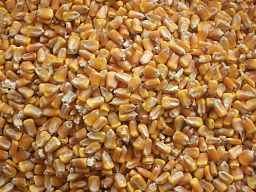
\includegraphics{images/cover.jpg}
\caption{}
\end{figure}

This is a book for beginners on commodity price analysis from a
fundamental perspective. These chapters are derived from my lecture
notes used to teach ACE 427: Commodity Price Analysis at the University
of Illinois The course itself is based an the outline given to me by
Scott Irwin, who has taught ACE 427 at the University of Illinois for
years.

This book is targeted at the upper level undergraduate student, or
professional beginning a career related to commodity markets. The
objective is to familiarize the reader with the sources of market
information and research commonly used by practicing professionals
working in the industry.

This book is updated with current information in the tables and figures
each time I teach the course. Previous versions of the book can be found
\href{https://github.com/mindymallory/PriceAnalysis/releases}{here}.

\section*{About the Author}\label{about-the-author}
\addcontentsline{toc}{section}{About the Author}

Mindy L. Mallory is an associate professor in the Department of
Agricultural and Consumer Economics at the University of Illinois in the
College of ACES.

Dr.~Mallory's research focuses on commodity markets and marketing
issues, especially related to commodity futures and options markets.
Topics of special interest include forecasting, liquidity costs, and
price discovery. Additionally, NSF-funded research examines how
portfolio theory from finance can be applied to help conservation groups
make informed resource allocation decisions in the face of climate
change.

\section*{Contact}\label{contact}
\addcontentsline{toc}{section}{Contact}

Mindy L. Mallory\\
mallorym at illinois dot edu\\
\url{https://mindymallory.github.io/}\\
\url{http://ace.illinois.edu/directory/mallorym}

© Mindy L. Mallory 2017

\chapter{Grain and Oilseed Markets}\label{grain-and-oilseed-markets}

Since commodities are natural things that are subject to biological
processes, you must first understand the basic biological processes
involved in the commodity's production in order to understand and
anticipate what happens to it's price. This chapter introduces the basic
production processes and timeline for major grains and oilseeds: Corn,
Soybeans, Hard Red Winter Wheat (KC wheat), Hard Red Spring Wheat
(Minneapolis wheat), and Soft Red Winter Wheat.

What's the difference between Sweet Corn one buys from the grocery store
and field corn (the focus of much of this course)?

Sweet corn has been bred so that the kernels contain a high sugar
content. It is harvested green (as you probably knew), and must be
consumed quickly, or processed by canning or freezing within a few
hours. After a few hours, the sugars in the kernels begin to turn to
starch.

Since sweet corn is harvested green and deteriorates rapidly, harvest
must take place quickly from start to finish.

\href{https://www.youtube.com/watch?v=4WEYDx82fG8}{Sweet Corn Harvest}

\section{Field Corn}\label{field-corn}

In the Corn Belt corn is planted from about March to May, and harvested
from September to October. Pollination usually occurs in July. Since
pollination is key to production and yield, new crop futures prices tend
to be highly variable in the months of June and July as weather patterns
and realizations of heat and rainfall mean the difference between a high
yielding year and low yielding year.

Of lesser concern, but still followed by market participants is the
weather during planting and harvest. Sometimes it is too wet, making it
difficult to get acreage planted in a timely manner. If corn is planted
too late it may suffer a yield penalty. Also, weather during harvest can
impact prices. If harvest time is very wet, it can make it difficult to
get the crop out and dry before it is damaged.

\href{https://www.youtube.com/watch?v=zuGVeXqTIaM}{Field Corn Harvest}

\begin{figure}[htbp]
\centering
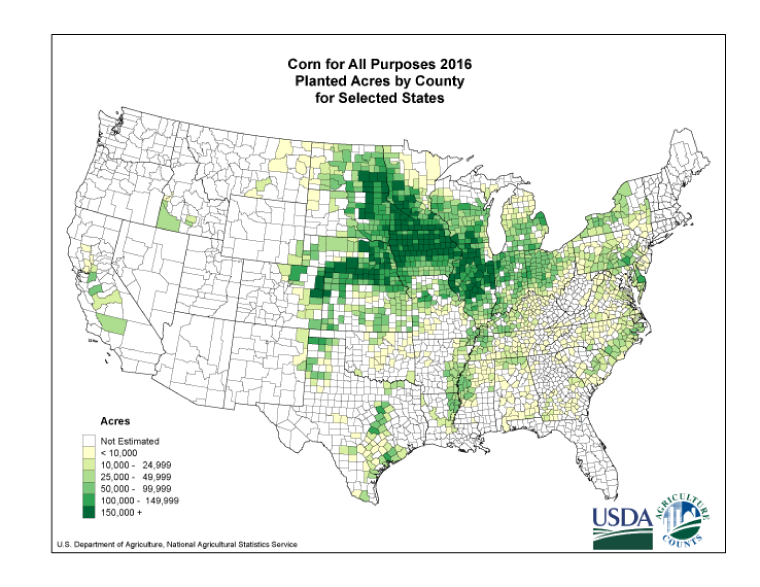
\includegraphics{images/Corn-PA-2016.png}
\caption{Figure 1: Corn Planted Acres 2016}
\end{figure}

\subsection{Recent Trends in Acreage, Yields, Production, and
Use}\label{recent-trends-in-acreage-yields-production-and-use}

Corn planted acres in the U.S. has varied from just under to just over
90 million acres in recent years. Farmers in the corn belt decide how
much of their land to plant to corn and how much to plant to soybeans.
So sometimes it is said in the spring that corn and soybeans are
`competing for acres' based on the relative new crop futures prices of
corn and soybeans. If corn is more profitable, farmers will shift some
acres toward corn, and if soybeans are more profitable farmers will
shift some acres toward soybeans. Because of this, years with high corn
planted acres tend to have lower soybeans planted acres and vice versa.

Seed hybrids and genetic modification have lead to dramatic increases in
yield over the last 100 years. Although, corn planted acres have been
relatively flat for a very long time, production has skyrocketed.

The following figures
\href{http://www.ers.usda.gov/topics/crops/corn/background.aspx}{come
from} the USDA's Economic Research Service (ERS).

\begin{figure}[htbp]
\centering
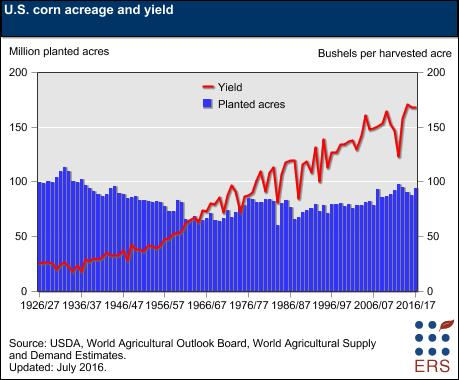
\includegraphics{images/Corn-PA-Yield.png}
\caption{Figure 1: Corn Planted Acres and Yield}
\end{figure}

Corn prices can be quite volatile, with prices and production highly
inversely related to one another.

\begin{figure}[htbp]
\centering
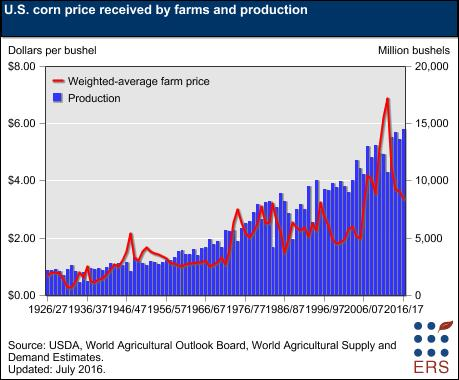
\includegraphics{images/Corn-PriceR-Production.png}
\caption{Figure 2: Corn Price Recieved by Farmers and Production}
\end{figure}

Corn is used in the U.S for a variety of purposes. Largest use
categories are feed (for livestock), and alcohol for fuel use (ethanol
blended with gasoline).

\begin{figure}[htbp]
\centering
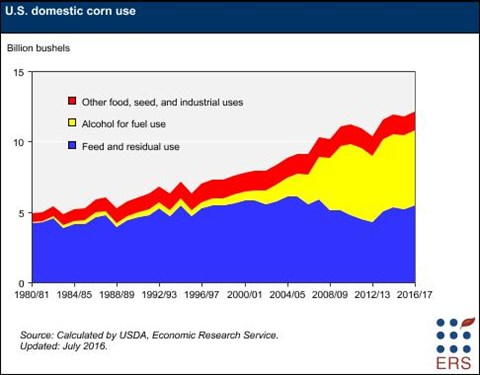
\includegraphics{images/Corn-Domestic-Use.png}
\caption{Figure 3: Corn Domestic Use Categories}
\end{figure}

Corn is a global commodity, and the U.S. is the worlds largest producer
and exporter of corn.

\begin{figure}[htbp]
\centering
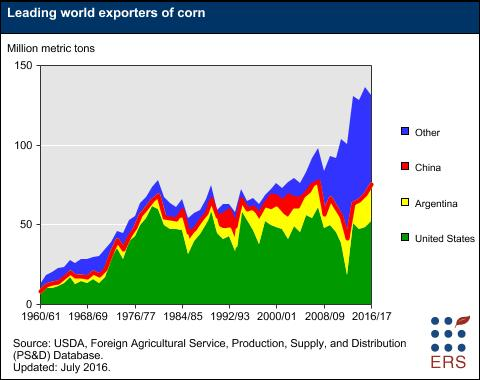
\includegraphics{images/Corn-World-Exporters.png}
\caption{Figure 4: Largest Exporters of Corn}
\end{figure}

\begin{figure}[htbp]
\centering
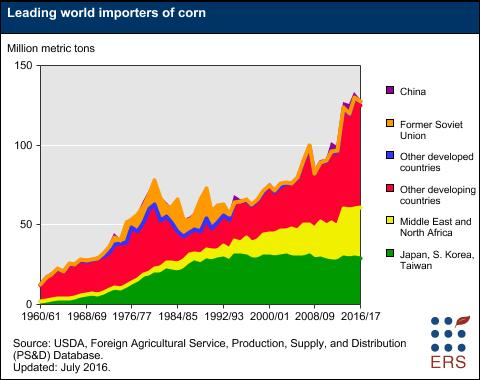
\includegraphics{images/Corn-World-Importers.png}
\caption{Figure 5: Largest Importers of Corn}
\end{figure}

\section{Soybeans}\label{soybeans}

Soybeans are planted later than corn, from about April to June. Weather
affects soybean production prospects and generates similar price
responses as it does for corn. Soybean prices, therefore are highly
dependent on what happens during the summer months. The following
figures
\href{http://www.ers.usda.gov/topics/crops/soybeans-oil-crops/background.aspx}{come
from} the USDS ERS.

\subsection{Recent Trends in Acreage, Yield, Production, and
Use}\label{recent-trends-in-acreage-yield-production-and-use}

Soybeans did not begin to be commercially grown in the U.S. until the
mid 20th century, but once it was introduced, acreage expanded rapidly.
Soybeans have also benefited from improved yields due to biotechnology.

\begin{figure}[htbp]
\centering
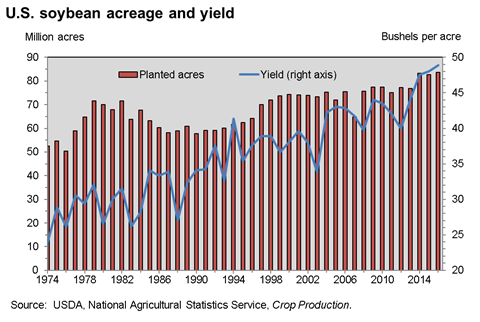
\includegraphics{images/Soy-Acres-Yield.png}
\caption{Figure 6: Soybean Planted Acres and Yield}
\end{figure}

Soybeans consumed in the U.S. are almost exclusively processed into
soybean meal and soybean oil, a process referred to as `crushing'.
Soybean meal is high in protein and used as an ingredient in livestock
feed. Soybean oil is used for a variety of things, but the bulk of it is
consumed as edible oil.

About half of the soybeans produced in the U.S. are exported, and more
than half of soybeans exported are
\href{http://farmdocdaily.illinois.edu/2015/03/footprint-of-chinese-demand-for-us-soybeans.html}{imported
by China}.

\begin{figure}[htbp]
\centering
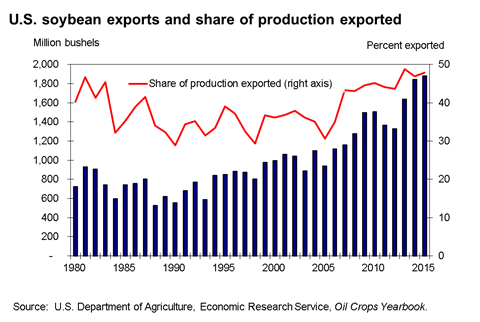
\includegraphics{images/Soy-Exports-Share-Production.png}
\caption{Figure 7: U.S. Soybean Exports}
\end{figure}

\section{Wheat}\label{wheat}

There are three main types of wheat grown in the U.S. Hard Red Winter
Wheat (HRW/KC Wheat), Hard Red Spring Wheat (HRS/Minneapolis wheat), and
Soft Red Winter Wheat (SRW/Chicago Wheat). Each of these types of wheat
have its own futures contract, are grown in distinct regions of the
country, and have different end uses. The main distinction between the
types of wheat is how much protein is contained in the kernels. This
variation in protein also determines what the variety of wheat is
ultimately used for.

\begin{figure}[htbp]
\centering
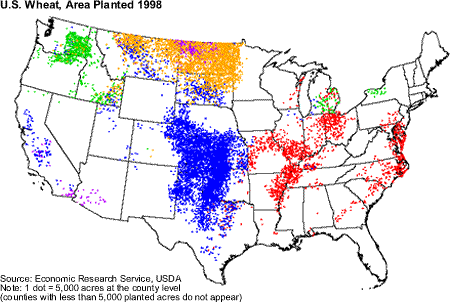
\includegraphics{images/Wheat-Growing-Areas.png}
\caption{Figure 8: Wheat Variety Growing Areas}
\end{figure}

(Source
\href{https://wayback.archive-it.org/5923/20120310141642/http://ers.usda.gov/Briefing/Wheat/maps.htm}{USDA-ERS})

Blue = HRW\\
Gold = HRS\\
Red = SRW

\subsection{Hard Red Winter Wheat}\label{hard-red-winter-wheat}

HRW wheat is planted in the fall and lays dormant or grows very little
during the winter. As temperatures rise in the spring, wheat plants
start to grow. It looks like grass before it is mature. During April and
May the wheat plants make `heads' where the wheat kernels grow. When the
plants die the grain is harvested.

HRW wheat is primarily used to make bread flour.

Hard Red Winter Wheat is sometime called Kansas City Wheat because the
Kansas City Board of Trade had a HRW wheat futures contract. The KCBOT
was recently bought by the CME Group, but HRW continues to be known as
KC wheat.

\begin{figure}[htbp]
\centering
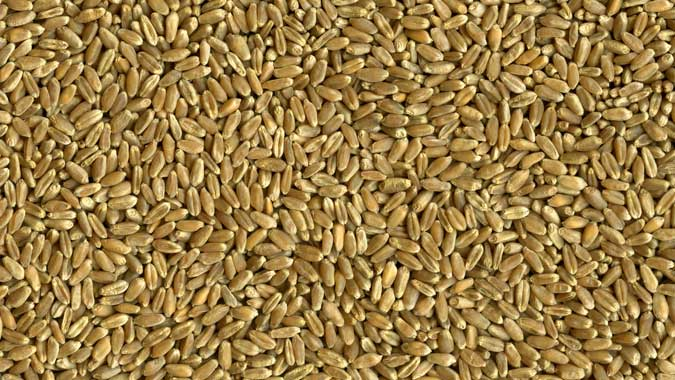
\includegraphics{images/HRW-Wheat.jpg}
\caption{Figure 9: Hard Red Winter Wheat}
\end{figure}

(Source
\href{https://www.gipsa.usda.gov/fgis/commgallery/gr_hrw.aspx}{USDA-GIPSA})

\subsection{Hard Red Spring Wheat}\label{hard-red-spring-wheat}

Hard red spring wheat is planted in the spring, around April or May and
is harvested in the fall, around September. It has the highest protein
content (13-16\%) of all the major wheat varieties, making it high in
gluten content, which is good for baking bread. It also is used to blend
with lower protein wheat flour varieties to increase the protein
content.

HRS wheat is referred to as Minneapolis Wheat because the
\href{http://www.mgex.com/}{Minneapolis Grain Exchange} offers a futures
contract in HRS wheat.

\begin{figure}[htbp]
\centering
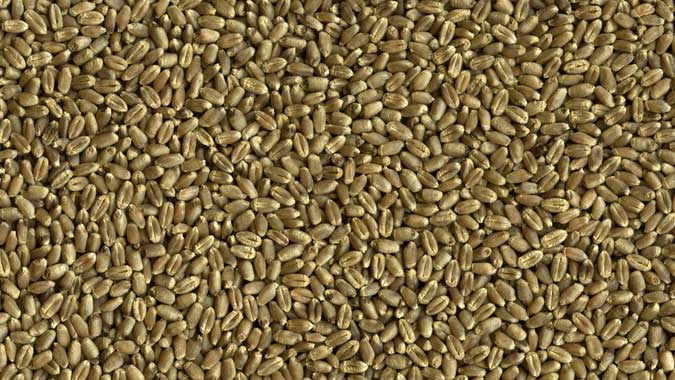
\includegraphics{images/HRS-Wheat.jpg}
\caption{Figure 10: Hard Red Spring Wheat}
\end{figure}

(Source
\href{https://www.gipsa.usda.gov/fgis/commgallery/gr_hrs.aspx}{USDA-GIPSA})

\subsection{Soft Red Winter Wheat}\label{soft-red-winter-wheat}

Soft Red Winter Wheat is planted in the fall, and is harvested in the
late spring, like HRW wheat. Soft red winter wheat is lower in protein
which makes is suitable for use in cakes, cookies, and crackers, where
high gluten content is not required.

SRW wheat is referred to as Chicago Wheat because the Chicago Board of
Trade offers a futures contract for SRW wheat.

\begin{figure}[htbp]
\centering
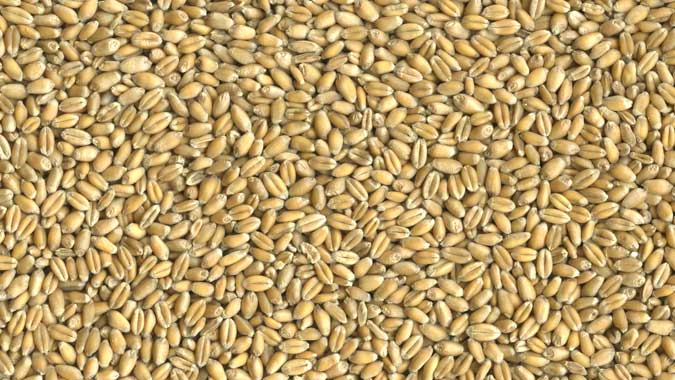
\includegraphics{images/SRW-Wheat.jpg}
\caption{Figure 11: Soft Red Winter Wheat}
\end{figure}

(Source
\href{https://www.gipsa.usda.gov/fgis/commgallery/gr_srw.aspx}{USDA-GIPSA})

\subsection{Protein Premiums and Wheat
Spreads}\label{protein-premiums-and-wheat-spreads}

If you follow wheat markets for long, you will hear discussion of
`protein premiums', that is because flour millers rarely use just one
kind of wheat to make their flour. They blend different types of wheat
together to make flours of varying protein and gluten levels.

Different varieties of wheat naturally have different protein levels, as
mentioned above. However, there is also a link between yield and protein
levels. When yields are high, wheat protein is lower. This means during
years where lower protein winter wheat has good yields, there is plenty
of wheat, but not necessarily enough protein. This causes the price of
higher protein wheat, like spring wheat, to rise against the price of
winter wheat. If winter wheat crops are smaller around the world, the
protein content is higher, and spring wheat may not enjoy a large
premium against winter wheat.

Because of this dynamic, the relative prices of Minneapolis, Kansas
City, and Chicago wheat futures are closely followed by stakeholders in
any of the wheat markets.

\chapter{Commodity Price Analysis and
Forecasting}\label{commodity-price-analysis-and-forecasting}

A commodity is a good that can be supplied without qualitative
differences. A bushel of wheat is regarded as a bushel of wheat
everywhere. Commodities are fully or partially fungible so that the
market treats a unit of good the same no matter who produced it or where
it was produced. Think of grain elevators, for example. Farmers bring
their grain to an elevator at harvest. Sometimes they sell it outright
to the elevator, but sometimes they pay the elevator to store it for
them. When the farmer decides to come get his grain out of storage do
you think he gets the exact same kernels he brought in? Of course that
would be impractical. The elevator just gives him back the same amount
of grain he brought in of the same quality. The farmer is happy because
the wheat is fungible. The grain he will be able to sell the grain he
took out just as easily as the grain he put in. This is in stark
contrast to differentiated goods where branding and quality make
important distinctions between goods, resulting in differentiated
demands. Just try to find someone indifferent between iPhone and
Android!

Since commodities are fungible, it also makes sense that prices of
commodities are determined by the entire (often global) market for the
good. They tend to be basic resources such as agricultural and food
products, metals, energy, an fibers. The fungibility of commodities
enables the commodity to be traded in centralized spot and futures
markets.

\subsection{Trasformation Over Space, Time, and
Form}\label{trasformation-over-space-time-and-form}

Commodities can undergo various transformations. Standard price analysis
usually groups these into three broad categories: Space, Time, and Form.
Studying a commodity's transformation over space comes about from the
fact that the production of a commodity is often concentrated in a
specific geographic location, while consumption of commodities is
usually dispersed. In order for traders to have incentive to move a
commodity from one location to another, a certain patter of prices must
prevail. In short, traders must be able to make a profit, or at least
break even in the business of moving a commodity from one location to
another.

Studying a commodity's transformation through time considers the nature
of prices required to provide incentive to store the commodity for use
at a later date (if it is possible to store the commodity - more on that
below), or incentive to bring the commodity to market. Using the example
of grain again, grain is produced once per year (in the United States),
but consumption of grains occurs all year long. In order for the market
to coordinate just the right amount of grain to be stored through time,
prices through time give incentive for those holding stocks of grain to
bring them to market or hold on longer.

Commodities can be transformed into completely different goods.
Sometimes this transformation creates new commodities; for example
soybeans are crushed into soybean oil and soybean meal - both of which
are considered commodities. Other times the transformation creates
products that are no longer considered commodities, where quality and
differentiation matters. Meat products are a good example of this.
Feeder cattle and live cattle are commodities, but through the slaughter
and processing process, the commodity becomes differentiated products -
different cuts of meat at the grocery store. Another example is coffee.
Green coffee beans are considered a commodity, but once they enter the
supply chain companies start transforming it by roasting, grinding, and
brewing the coffee. Starbucks, for example, does not sell a commodity.
Their product is highly differentiated and they market the fact that
their product is highly differentiated in the marketplace.

\section{Storable and Nonstorable}\label{storable-and-nonstorable}

A key difference among commodities is their degree of storability. Some
can be stored for long periods of time:

\begin{itemize}
\tightlist
\item
  Corn
\item
  Soybeans
\item
  Wheat
\item
  Peanuts
\item
  Crude Oil
\item
  Natural Gas
\end{itemize}

Others are highly perishable or otherwise non-storeable :

\begin{itemize}
\tightlist
\item
  Hogs
\item
  Cattle
\item
  Milk
\item
  Potatoes
\item
  Apples
\item
  Tomatoes
\item
  Electricity
\end{itemize}

The storability of a commodity has profound implications on market
prices. With storable commodities, they can be stored from one period to
the next. This means the prices in one period must be related to prices
in another period because those holding stocks of the commodity will
constantly calculating their expectation of when best to sell - now or
later. With non-storable commodities, prices can only be affected by the
current supply of the commodity, since past supply cannot be brought
forward.

\section{Commodity Prices}\label{commodity-prices}

Commodity prices are important both economically and politically in
almost all countries. Commodity prices strongly influence farm income,
and this can be quite volatile from year-to-year. The United States has
a long history of policies aimed at smoothing out the price volatility
and income volatility for farmers.

\begin{itemize}
\tightlist
\item
  Price supports
\item
  Revenue supports
\item
  Subsidized crop insurance programs
\end{itemize}

Some countries' economies rely heavily on the export of various kinds of
commodities. This leaves their economic growth and prosperity subject to
volatility in commodity prices. In other countries, particularly in the
developing world, a large share of the population for still engages in
agricultural production for their livelihood. For these people,
commodity prices determine the bulk of their income, and incomes of the
poor is a primary concern in developing economies.

\subsection{Forecasting Commodity Prices in
Business}\label{forecasting-commodity-prices-in-business}

Some companies business model leaves them exposed to risk that comes
from price volatility and spend considerable resources forecasting
prices. These tend to be companies that deal directly in commodities and
need to hedge risks. Some examples include:

\begin{itemize}
\tightlist
\item
  ADM
\item
  Cargill
\item
  Caterpillar
\item
  ConAgra
\item
  Kraft
\item
  Weyerhauser
\end{itemize}

There are consistent employment opportunities for students trained in
price analysis and forecasting, and a growing interest in expertise in
risk management strategies.

\subsection{Price Analysis versus
Forecasting}\label{price-analysis-versus-forecasting}

Price analysis and price forecasting are not exactly the same thing.
Price analysis tends to be backward looking, while price forecasting is
forward looking.

Price Analysis: - Goal is to understand the complex array of forces that
influence the level and behavior of commodity prices - Aids in
understanding performance of commodity markets - Aids in the development
of policy, and is a key component of the policy analysis that leads the
a policy's promotion or demise

Price Forecasting: - Goal is to reliably and accurately forecast future
price levels of commodities - The forecasts can be used in marketing and
speculative strategies

\section{Forecasting Basics}\label{forecasting-basics}

\begin{enumerate}
\def\labelenumi{\arabic{enumi}.}
\item
  All meaningful forecasts guide decisions

  \begin{itemize}
  \tightlist
  \item
    An awareness of the nature of the decisions will impact the design,
    use, and evaluation of the forecasting process
  \end{itemize}
\item
  Form of forecast statement

  \begin{description}
  \item[Directional forecast]
  Fed steer prices for the first quarter of 2016 will be down compared
  to the same quarter last year.
  \item[Simple point forecast]
  Fed steer prices for the fist quarter of 2016 = \$150/cwt.
  \item[Interval forecast]
  Fed steer prices for the first quarter of 2016 = \$140-\$160/cwt
  \item[Confidence interval forecast]
  We are 80\% confident that fed steer prices fore the first quarter of
  2016 will be between \$140-\$160/cwt
  \item[Density forecast]
  Provides entire probability distribution of forecast price.
  \end{description}
\item
  Forecast horizon

  \begin{itemize}
  \item
    Forecast horizon is the number of periods between today and the date
    of the forecast made.
  \item
    If dealing with monthly data:

    \begin{itemize}
    \tightlist
    \item
      1-step ahead = One month beyond the current month
    \item
      2-step ahead = two months beyond the current month
    \item
      \texttt{h}-step ahead = \texttt{h} months beyond the current month
    \end{itemize}
  \item
    More complex situations are common in crop market forecasting

    \begin{itemize}
    \tightlist
    \item
      Typical unit of time is a `marketing year'.{[}\^{}More on the
      marketing year in Chapter 3{]}
    \item
      Forecasts are typically updated monthly.
    \end{itemize}
  \end{itemize}
\item
  Parsimony principle

  \begin{itemize}
  \tightlist
  \item
    Other things equal, simple approaches are preferred
  \item
    Also known as
    \href{https://en.wikipedia.org/wiki/Occam\%27s_razor}{Occam's Razor}
  \end{itemize}

  \begin{quote}
  The Principle States that among competing hypotheses that predict
  equally well, the one with the fewest assumptions should be selected.
  Other, more complicated solutions may ultimately prove to provide
  better predictions, but - in the absence of differences in predictive
  ability - the fewer assumptions that are made, the better. (Source:
  \href{https://en.wikipedia.org/wiki/Occam\%27s_razor}{Wikipedia})
  \end{quote}

  \begin{itemize}
  \item
    Simple approaches tend to work best in real world applications

    \begin{itemize}
    \tightlist
    \item
      Based on decades of experience and research
    \item
      Simpler models can be estimated more precisely
    \item
      Because simpler models can be more easily interpreted and
      understood, unusual behavior and outcomes can be more easily
      spotted.
    \end{itemize}
  \item
    It is easier to communicate the basic behavior and design of simple
    approaches, so they are more likely to be used by decision-makers.
  \item
    Simple approaches lessen the chances of data mining problems.

    \begin{itemize}
    \tightlist
    \item
      If a complex model is tailored to fit historical data very well,
      but does not capture the true nature of the data process,
      forecasts will perform poorly.
    \end{itemize}
  \end{itemize}
\end{enumerate}

We focus on two types of ``simple'' forecasting methods.

\begin{enumerate}
\def\labelenumi{\arabic{enumi}.}
\item
  Fundamental analysis: use of economic models and data on production,
  consumption, income, etc. to forecast prices. You will recognize this
  approach as balance sheet analysis in chapter 3.
\item
  Reduced form time-series econometric: use of statistical econometric
  models that features minimal inputs beyond a few recent prices to
  generate a forecasting model.
\end{enumerate}

Not covered here, but a method used widely by day-traders and other
market participants is technical analysis, which is the use of past
price patterns to predict future price movement. There are scores of
books on the topic of technical analysis, if interested.

\subsection{Commodity Production
Cycles}\label{commodity-production-cycles}

The production of agricultural commodities is bound by the biological
traits of the life cycle. Forecasting prices requires an awareness of
key seasons, and problems that can arise during each phase of the life
cycle.

\section{Long Term Trends}\label{long-term-trends}

It is useful to begin our exploration of agricultural prices from a long
term historical perspective. The figure below is monthly prices received
by farmers in the U.S. from 1908 to 2015. By simple visual inspection
there seems to be three periods of stable prices, from 1908-1973,
1974-2006, and 2007-present. Although the most recent period seems to be
the most volatile and provides less confidence that a similar pattern
will persist going forward.

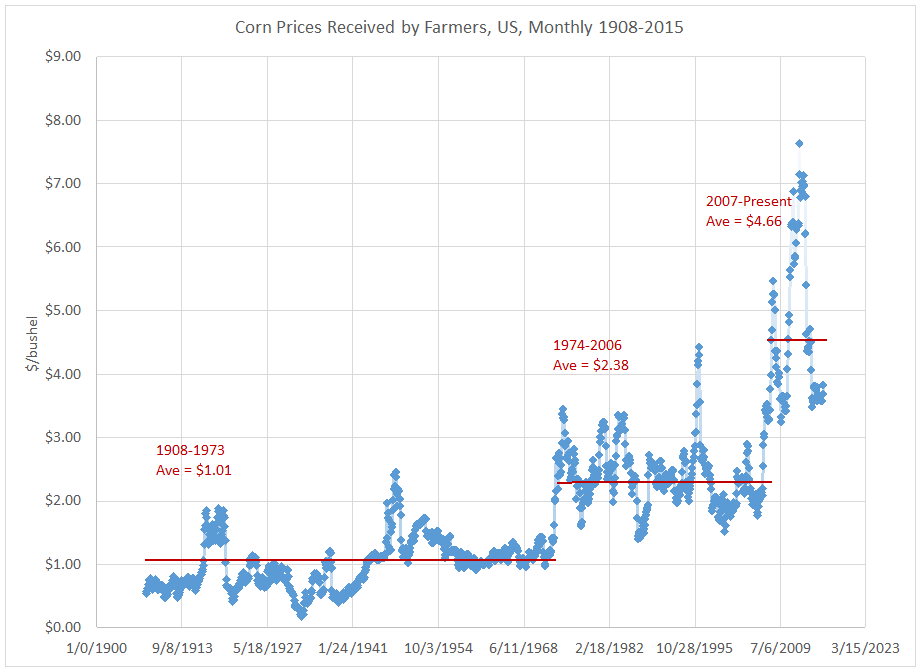
\includegraphics{Excel-files/IntroductiontoCommodity_files/image001.png}
Source(\url{http://www.nass.usda.gov/})

Now lets zoom in on the 1974-2015 periods.

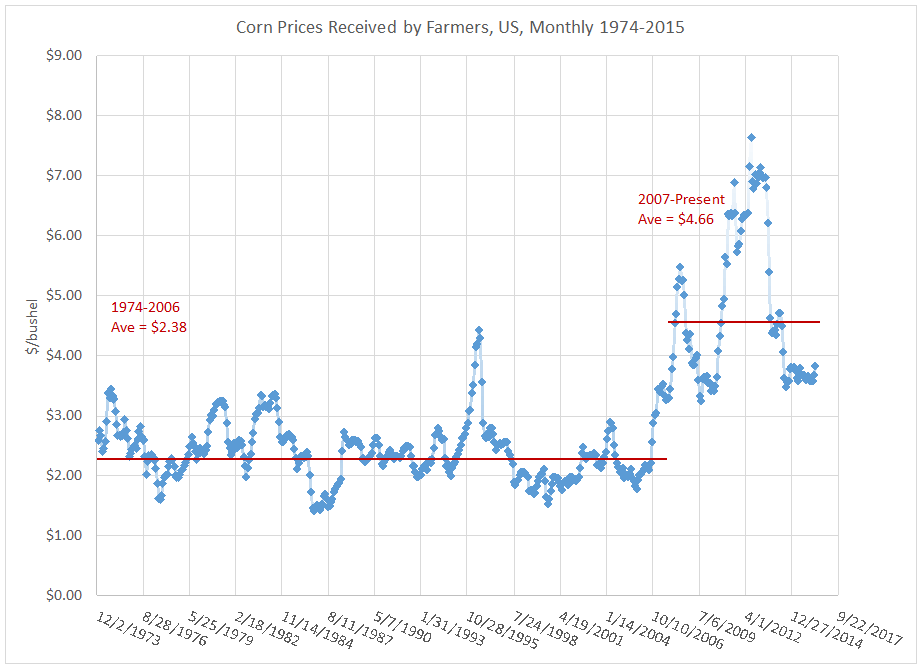
\includegraphics{Excel-files/IntroductiontoCommodity_files/image003.png}
Source(\url{http://www.nass.usda.gov/})

Looking at these two charts together, there is a clear run-up in prices
in the 1970's and again around 2006-2007. What caused these seemingly
permanent price hikes?

\section{Readings}\label{readings}

\begin{description}
\item[\href{pdf-Readings/ers-amber-waves-2009-ag-com-pr-sp-1970s-1990s.pdf}{Agricultural
Commodity Price Spikes in the 1970s and 1990s: Valuable Lessons for
Today}]
This article was published by staff at the United States Department of
Agriculture's Economic Research Service. They look at historical corn
prices and provide some perspective about what caused the price
increases in the 1970's and mid-2000's.
\item[\href{http://www.choicesmagazine.org/magazine/pdf/article_56.pdf}{Market
Instability in a New Era of Corn, Soybean, and Wheat Prices}]
Scott Irwin and Darrel good had an article in Choices magazine, that
examined the price `eras' we described in this chapter. They also
discuss the causes of the price paradigm shifts. They argued in 2009
that the new `era' of crop prices were here to stay, and history has
bore this out so far.
\end{description}

\section{Exercises}\label{exercises}

\begin{enumerate}
\def\labelenumi{\arabic{enumi}.}
\item
  From the readings, describe causes of the rapid and persistent
  increase in prices in the early 1970's.
\item
  From the readings, describe the causes of the rapid and persistent
  increase in prices in 2006/2007.
\item
  In your opinion, is there evidence that price trends will hold at
  their current levels?
\end{enumerate}

\chapter{How to Find Information}\label{how-to-find-information}

This chapter serves as an introduction to real-time and historical data
sources, as well as an introduction to the analysts that conduct price
analysis professionally and help us make sense of commodity prices.
First, we will introduce the reader to some entities that provide market
commentary and price analysis. Next, we will provide a very brief
introduction to futures markets as the source of real-time price
information for commodities. This section also covers where and how to
obtain current futures price quotes. In the section that follows we
cover sources for historical data such as the United States Department
of Agriculture and others. These sources will be useful in developing
fundamental price models in later chapters. The goal of this chapter is
to get the reader up to speed on where to get commodity price data and
reading the professional analysis daily. The more you follow commodity
markets, the more you learn. Absorb the insights of the professionals
who live and breath commodity markets every day, and you will begin to
have a feel for what price analysis is all about and how it works.

\section{Market Commentary}\label{market-commentary}

The best way to learn commodity price analysis is to listen to the
professionals who provide commentary on the markets on a regular basis.
Land grant universities located in major commodity producing states all
have components of their outreach programs dedicated to market
commentary. The University of Illinois' web extension program, FARMDOC,
is particularly good. Also, public radio in major commodity producing
areas has excellent coverage. Champaign-Urbana's WILL, and Iowa Public
Televisions' Market to Market are very good. There are \emph{many} other
great sources providing regular commentary, but this will get the reader
started.

\begin{longtable}[]{@{}lll@{}}
\caption{Table 1. Resources for Commodity Market
Commentary}\tabularnewline
\toprule
\begin{minipage}[b]{0.14\columnwidth}\raggedright\strut
Outlet\strut
\end{minipage} & \begin{minipage}[b]{0.25\columnwidth}\raggedright\strut
Description\strut
\end{minipage} & \begin{minipage}[b]{0.23\columnwidth}\raggedright\strut
Link\strut
\end{minipage}\tabularnewline
\midrule
\endfirsthead
\toprule
\begin{minipage}[b]{0.14\columnwidth}\raggedright\strut
Outlet\strut
\end{minipage} & \begin{minipage}[b]{0.25\columnwidth}\raggedright\strut
Description\strut
\end{minipage} & \begin{minipage}[b]{0.23\columnwidth}\raggedright\strut
Link\strut
\end{minipage}\tabularnewline
\midrule
\endhead
\begin{minipage}[t]{0.14\columnwidth}\raggedright\strut
Farmdoc Daily\strut
\end{minipage} & \begin{minipage}[t]{0.25\columnwidth}\raggedright\strut
Extension web presence by the department of ACE\strut
\end{minipage} & \begin{minipage}[t]{0.23\columnwidth}\raggedright\strut
\href{http://farmdocdaily.illinois.edu}{farmdocdaily.illinois.edu}\strut
\end{minipage}\tabularnewline
\begin{minipage}[t]{0.14\columnwidth}\raggedright\strut
WILL Agriculture\strut
\end{minipage} & \begin{minipage}[t]{0.25\columnwidth}\raggedright\strut
WILL and the University of Illinois Extension\strut
\end{minipage} & \begin{minipage}[t]{0.23\columnwidth}\raggedright\strut
\href{http://will.illinois.edu/agriculture}{will.illinois.edu/agriculture}\strut
\end{minipage}\tabularnewline
\begin{minipage}[t]{0.14\columnwidth}\raggedright\strut
Market to Market\strut
\end{minipage} & \begin{minipage}[t]{0.25\columnwidth}\raggedright\strut
Agricultural programming by Iowa Public Television\strut
\end{minipage} & \begin{minipage}[t]{0.23\columnwidth}\raggedright\strut
\href{http://www.iptv.org/mtom/}{www.iptv.org/mtom/}\strut
\end{minipage}\tabularnewline
\bottomrule
\end{longtable}

\section{Futures Price Quotes}\label{futures-price-quotes}

Futures contracts (contracts to buy/sell a specific quantity of, say,
corn at a specific price on a specific date in the future) can be
distinguished from forward contracts in that quantity and quality are
standardized. This facilitates the ability of futures contracts to be
traded on an exchange. Whereas a forward contract has specific
counter-parties (buyers and sellers), with futures contracts the
exchange becomes the seller to every buyer and the buyer to every
seller. If enough market participants are present it is very easy to get
into and out of these futures contracts because you do not have to come
to an agreement with the original buyer/seller. You simply take an
offsetting position (sell if you originally bought and buy if you
originally sold) at the currently prevailing price. The exchange takes
your contractual obligation off the books and you just pay (or receive)
the difference in price between when you bought and when you sold. Fully
understanding the function of futures markets is well beyond the scope
of this book, but the interested reader is encouraged to refer to Kub
\citeyearpar{kub2012Mastering} for a practical introduction and Hull
\citep{hull1991introduction} for a more technical approach.

\subsection{Futures Data Sources}\label{futures-data-sources}

For agricultural commodities in the United States, the
\href{http://www.cmegroup.com/}{CME Group} is the most important futures
exchange for price discovery. Grain and oil-seed contracts traded at the
CME Group include corn, soybeans, soybean oil, soybean meal, soft red
winter wheat, hard red winter wheat. They also list futures contracts
for livestock products such as live cattle, lean hogs, and feeder
cattle. `Soft' commodities that trade on the CME Group are cocoa,
coffee, and sugar. The CME Group also lists energy commodity products
for crude oil, natural gas, ethanol, and other products. This book will
focus most intently on the grain and oil-seed contracts, with some
topics related to the cattle and energy contracts considered. Many of
these futures contracts are considered to be the main price setting
function for the commodity in the world. Chicago Board of Trade (owned
by the CME Group) futures prices of corn and soybeans are considered the
`World Price' of corn and soybeans. Meaning that all over the globe,
prices for these commodities are set based on what the price of corn and
soybeans are trading on the CME Group exchanges.

Real-time (10-min delay) data can be obtained directly from the CME
Group's website. There you can view the most recent quotes, and some
charting capability is provided as well. Typically, however, it is more
convenient to obtain market quotes from third party vendors like
\href{http://finance.yahoo.com/}{Yahoo Finance},
\href{https://www.quandl.com/collections/futures}{Quandl},
\href{http://www.barchart.com/futures/marketoverview}{barchart}
(subscription required), or others. Those sources offer a more flexible
interface for viewing on the web, and provide utility to download recent
price history.

\subsection{Futures Symbols and Looking up Data by Contract
Expiration}\label{futures-symbols-and-looking-up-data-by-contract-expiration}

Contracts for several different expiry dates trade at the same time.
There is a useful shorthand for finding contracts for a specific
commodity and expiration month that varies only slightly among data
vendors; all follow a general convention for building futures ticker
symbols customizing only to meet the needs of their individual systems.
The table below lists selected grain and oilseed, livestock, and energy
contract symbols, expiration symbols, and common ticker formats used to
search for price quotes. For example, the first row of the table
illustrates that the general convention for representing the CBOT corn
futures contract expiring in December of 2017 is CZ17. The first letter
represents the commodity symbol, C for corn; the second letter
represents the expiration month, Z for December; and the final two
numerals represent the year of expiry, 17 for 2017.

\begin{longtable}[]{@{}lcllll@{}}
\caption{Table 2. Conventions for Building Futures Contract Ticker
Symbols for Selected Commodities}\tabularnewline
\toprule
\begin{minipage}[b]{0.07\columnwidth}\raggedright\strut
Commodity\strut
\end{minipage} & \begin{minipage}[b]{0.07\columnwidth}\centering\strut
Symbol\strut
\end{minipage} & \begin{minipage}[b]{0.32\columnwidth}\raggedright\strut
Expiration Months and Symbol\strut
\end{minipage} & \begin{minipage}[b]{0.13\columnwidth}\raggedright\strut
General Ticker\strut
\end{minipage} & \begin{minipage}[b]{0.13\columnwidth}\raggedright\strut
Yahoo Finance Ticker\strut
\end{minipage} & \begin{minipage}[b]{0.13\columnwidth}\raggedright\strut
Quandl Ticker\strut
\end{minipage}\tabularnewline
\midrule
\endfirsthead
\toprule
\begin{minipage}[b]{0.07\columnwidth}\raggedright\strut
Commodity\strut
\end{minipage} & \begin{minipage}[b]{0.07\columnwidth}\centering\strut
Symbol\strut
\end{minipage} & \begin{minipage}[b]{0.32\columnwidth}\raggedright\strut
Expiration Months and Symbol\strut
\end{minipage} & \begin{minipage}[b]{0.13\columnwidth}\raggedright\strut
General Ticker\strut
\end{minipage} & \begin{minipage}[b]{0.13\columnwidth}\raggedright\strut
Yahoo Finance Ticker\strut
\end{minipage} & \begin{minipage}[b]{0.13\columnwidth}\raggedright\strut
Quandl Ticker\strut
\end{minipage}\tabularnewline
\midrule
\endhead
\begin{minipage}[t]{0.07\columnwidth}\raggedright\strut
Corn\strut
\end{minipage} & \begin{minipage}[t]{0.07\columnwidth}\centering\strut
C\strut
\end{minipage} & \begin{minipage}[t]{0.32\columnwidth}\raggedright\strut
March (H), May (K), July (N), September (U), December (Z)\strut
\end{minipage} & \begin{minipage}[t]{0.13\columnwidth}\raggedright\strut
CZ17, December 2017 Corn\strut
\end{minipage} & \begin{minipage}[t]{0.13\columnwidth}\raggedright\strut
\href{https://finance.yahoo.com/quote/cz17.cbt}{CZ17.cbt}\strut
\end{minipage} & \begin{minipage}[t]{0.13\columnwidth}\raggedright\strut
\href{https://www.quandl.com/data/CME/CZ2017-Corn-Futures-December-2017-CZ2017}{CME/CZ2017}\strut
\end{minipage}\tabularnewline
\begin{minipage}[t]{0.07\columnwidth}\raggedright\strut
Soybeans\strut
\end{minipage} & \begin{minipage}[t]{0.07\columnwidth}\centering\strut
S\strut
\end{minipage} & \begin{minipage}[t]{0.32\columnwidth}\raggedright\strut
January (F), March (H), May (K), July (N), August (Q), September (U),
November (X)\strut
\end{minipage} & \begin{minipage}[t]{0.13\columnwidth}\raggedright\strut
SX17, November 2017 Soybean\strut
\end{minipage} & \begin{minipage}[t]{0.13\columnwidth}\raggedright\strut
\href{http://finance.yahoo.com/quote/SX17.CBT/?p=SX17.CBT}{SX17.cbt}\strut
\end{minipage} & \begin{minipage}[t]{0.13\columnwidth}\raggedright\strut
\href{https://www.quandl.com/data/CME/SX2017-Soybean-Futures-November-2017-SX2017}{CME/SX2017}\strut
\end{minipage}\tabularnewline
\begin{minipage}[t]{0.07\columnwidth}\raggedright\strut
Canola/Rapeseed\strut
\end{minipage} & \begin{minipage}[t]{0.07\columnwidth}\centering\strut
RS\strut
\end{minipage} & \begin{minipage}[t]{0.32\columnwidth}\raggedright\strut
January (F), March (H), May (K), July (N), November (X)\strut
\end{minipage} & \begin{minipage}[t]{0.13\columnwidth}\raggedright\strut
RSX17, November 2017\strut
\end{minipage} & \begin{minipage}[t]{0.13\columnwidth}\raggedright\strut
\href{http://www.barchart.com/quotes/futures/RSX17}{RSX17}
(Barchart)\strut
\end{minipage} & \begin{minipage}[t]{0.13\columnwidth}\raggedright\strut
\href{https://www.quandl.com/data/ICE/RSX2017-Canola-Futures-November-2017-RSX2017}{ICE/RSX2017}\strut
\end{minipage}\tabularnewline
\begin{minipage}[t]{0.07\columnwidth}\raggedright\strut
HRW Wheat\strut
\end{minipage} & \begin{minipage}[t]{0.07\columnwidth}\centering\strut
KW\strut
\end{minipage} & \begin{minipage}[t]{0.32\columnwidth}\raggedright\strut
March (H), May (K), July (N), September (U), December (Z)\strut
\end{minipage} & \begin{minipage}[t]{0.13\columnwidth}\raggedright\strut
KWN18, July 2018 KC Wheat\strut
\end{minipage} & \begin{minipage}[t]{0.13\columnwidth}\raggedright\strut
\href{https://finance.yahoo.com/quote/KWN18.CBT?p=KWN18.CBT}{KWN18.cbt}\strut
\end{minipage} & \begin{minipage}[t]{0.13\columnwidth}\raggedright\strut
\href{https://www.quandl.com/data/CME/KWN2018-KC-HRW-Wheat-Futures-July-2018-KWN2018}{CME/KWN2018}\strut
\end{minipage}\tabularnewline
\begin{minipage}[t]{0.07\columnwidth}\raggedright\strut
SRW Wheat\strut
\end{minipage} & \begin{minipage}[t]{0.07\columnwidth}\centering\strut
W\strut
\end{minipage} & \begin{minipage}[t]{0.32\columnwidth}\raggedright\strut
March (H), May (K), July (N), September (U), December (Z)\strut
\end{minipage} & \begin{minipage}[t]{0.13\columnwidth}\raggedright\strut
WZ17, December 2017 SRW Wheat\strut
\end{minipage} & \begin{minipage}[t]{0.13\columnwidth}\raggedright\strut
\href{https://finance.yahoo.com/quote/wz17.cbt}{WZ17.cbt}\strut
\end{minipage} & \begin{minipage}[t]{0.13\columnwidth}\raggedright\strut
\href{https://www.quandl.com/data/CME/WZ2017-Wheat-Futures-December-2017-WZ2017}{CME/WZ2017}\strut
\end{minipage}\tabularnewline
\begin{minipage}[t]{0.07\columnwidth}\raggedright\strut
HRS Wheat\strut
\end{minipage} & \begin{minipage}[t]{0.07\columnwidth}\centering\strut
MW\strut
\end{minipage} & \begin{minipage}[t]{0.32\columnwidth}\raggedright\strut
March (H), May (K), July (N), September (U), December (Z)\strut
\end{minipage} & \begin{minipage}[t]{0.13\columnwidth}\raggedright\strut
MWZ17, Dec 2017 Minn Wheat\strut
\end{minipage} & \begin{minipage}[t]{0.13\columnwidth}\raggedright\strut
NA\strut
\end{minipage} & \begin{minipage}[t]{0.13\columnwidth}\raggedright\strut
\href{https://www.quandl.com/data/MGEX/MWZ2017-Minneapolis-Hard-Red-Spring-Wheat-Futures-December-2017-MWZ2017}{MGE/MWZ2017}\strut
\end{minipage}\tabularnewline
\begin{minipage}[t]{0.07\columnwidth}\raggedright\strut
Live Cattle\strut
\end{minipage} & \begin{minipage}[t]{0.07\columnwidth}\centering\strut
LC\strut
\end{minipage} & \begin{minipage}[t]{0.32\columnwidth}\raggedright\strut
Feb (G), Apr (J), Jun (M), Aug (Q), Oct (V), Dec (Z)\strut
\end{minipage} & \begin{minipage}[t]{0.13\columnwidth}\raggedright\strut
LCZ17, December 2017 Live Cattle\strut
\end{minipage} & \begin{minipage}[t]{0.13\columnwidth}\raggedright\strut
\href{http://finance.yahoo.com/quote/LCZ17.CME/?p=LCZ17.CME}{LCZ17.CME}\strut
\end{minipage} & \begin{minipage}[t]{0.13\columnwidth}\raggedright\strut
\href{https://www.quandl.com/data/CME/LCZ2017-Live-Cattle-Futures-December-2017-LCZ2017}{CME/LCZ2017}\strut
\end{minipage}\tabularnewline
\begin{minipage}[t]{0.07\columnwidth}\raggedright\strut
Lean Hogs\strut
\end{minipage} & \begin{minipage}[t]{0.07\columnwidth}\centering\strut
LH\strut
\end{minipage} & \begin{minipage}[t]{0.32\columnwidth}\raggedright\strut
Feb (G), Apr (J), May (K), Jun (M), Jul (N), Aug (Q), Oct (V), Dec
(Z)\strut
\end{minipage} & \begin{minipage}[t]{0.13\columnwidth}\raggedright\strut
LHZ17, December 2017 Lean Hogs\strut
\end{minipage} & \begin{minipage}[t]{0.13\columnwidth}\raggedright\strut
\href{http://finance.yahoo.com/quote/LHZ17.CME/?p=LHZ17.CME}{LHZ17.cme}\strut
\end{minipage} & \begin{minipage}[t]{0.13\columnwidth}\raggedright\strut
\href{https://www.quandl.com/data/CME/LNZ2017-Lean-Hog-Futures-December-2017-LNZ2017}{CME/LNZ2017}\strut
\end{minipage}\tabularnewline
\begin{minipage}[t]{0.07\columnwidth}\raggedright\strut
Crude Oil\strut
\end{minipage} & \begin{minipage}[t]{0.07\columnwidth}\centering\strut
CL\strut
\end{minipage} & \begin{minipage}[t]{0.32\columnwidth}\raggedright\strut
All months\strut
\end{minipage} & \begin{minipage}[t]{0.13\columnwidth}\raggedright\strut
CLZ17 Dec 2017 Light Sweet Crude Oil\strut
\end{minipage} & \begin{minipage}[t]{0.13\columnwidth}\raggedright\strut
\href{http://finance.yahoo.com/quote/CLZ17.NYM/?p=CLZ17.NYM}{CLZ17.nym}\strut
\end{minipage} & \begin{minipage}[t]{0.13\columnwidth}\raggedright\strut
\href{https://www.quandl.com/data/CME/CLZ2017-Crude-Oil-Futures-September-2017-CLZ2017}{CME/CLZ2017}\strut
\end{minipage}\tabularnewline
\begin{minipage}[t]{0.07\columnwidth}\raggedright\strut
RBOB Gasoline\strut
\end{minipage} & \begin{minipage}[t]{0.07\columnwidth}\centering\strut
RB\strut
\end{minipage} & \begin{minipage}[t]{0.32\columnwidth}\raggedright\strut
All months\strut
\end{minipage} & \begin{minipage}[t]{0.13\columnwidth}\raggedright\strut
RBZ17, Dec 2017 RBOB Gas\strut
\end{minipage} & \begin{minipage}[t]{0.13\columnwidth}\raggedright\strut
\href{https://finance.yahoo.com/quote/RBZ17.NYM}{RBZ17.nym}\strut
\end{minipage} & \begin{minipage}[t]{0.13\columnwidth}\raggedright\strut
\href{https://www.quandl.com/data/CME/RBZ2017-RBOB-Gasoline-Physical-Futures-December-2017-RBZ2017}{CME/RBZ2017}\strut
\end{minipage}\tabularnewline
\begin{minipage}[t]{0.07\columnwidth}\raggedright\strut
Heating Oil\strut
\end{minipage} & \begin{minipage}[t]{0.07\columnwidth}\centering\strut
HO\strut
\end{minipage} & \begin{minipage}[t]{0.32\columnwidth}\raggedright\strut
All months\strut
\end{minipage} & \begin{minipage}[t]{0.13\columnwidth}\raggedright\strut
HOZ17, Dec 2017 HO (Ultra low sulfur diesel)\strut
\end{minipage} & \begin{minipage}[t]{0.13\columnwidth}\raggedright\strut
\href{https://finance.yahoo.com/quote/HOZ17.NYM/?p=HOZ17.NYM}{HOZ17.NYM}\strut
\end{minipage} & \begin{minipage}[t]{0.13\columnwidth}\raggedright\strut
\href{https://www.quandl.com/data/CME/HOZ2017-NY-Harbor-ULSD-Futures-December-2017-HOZ2017}{CME/HOZ2017}\strut
\end{minipage}\tabularnewline
\begin{minipage}[t]{0.07\columnwidth}\raggedright\strut
Ethanol\strut
\end{minipage} & \begin{minipage}[t]{0.07\columnwidth}\centering\strut
EH\strut
\end{minipage} & \begin{minipage}[t]{0.32\columnwidth}\raggedright\strut
All Months\strut
\end{minipage} & \begin{minipage}[t]{0.13\columnwidth}\raggedright\strut
EHZ17, Dec 2017 Ethanol Futures\strut
\end{minipage} & \begin{minipage}[t]{0.13\columnwidth}\raggedright\strut
\href{https://finance.yahoo.com/quote/EHZ17-2.CBT/futures?p=EHZ17-2.CBT}{EHZ17.CBT}\strut
\end{minipage} & \begin{minipage}[t]{0.13\columnwidth}\raggedright\strut
\href{https://www.quandl.com/data/CME/EHZ2017-Ethanol-Futures-December-2017-EHZ2017}{CME/EHZ2017}\strut
\end{minipage}\tabularnewline
\bottomrule
\end{longtable}

While every market participant needs to know the current price,
forecasting and decision making requires the study of historical prices
and other important market variables. Historical futures price data is
available for free and from subscription based services from
\href{https://quandl.com}{Quandl} and
\href{https://barchart.com}{Barchart} mentioned in the paragraph above.
Historical
\href{http://farmdoc.agricharts.com/markets/historic.php}{futures price
data} and
\href{http://www.farmdoc.illinois.edu/manage/pricehistory/price_history.html}{average
price recieved} is also available from
\href{http://www.farmdoc.illinois.edu}{farmdoc}, the online extension
presence of the University of Illinois'
\href{http://ace.illinois.edu/}{Agricultural and Consumer Economics}
department.

Table 3 provides some links to spread charts for commodity spreads we
will cover in this class.

\begin{longtable}[]{@{}ll@{}}
\caption{Table 3. Commodity Spreads}\tabularnewline
\toprule
\begin{minipage}[b]{0.10\columnwidth}\raggedright\strut
Spread\strut
\end{minipage} & \begin{minipage}[b]{0.10\columnwidth}\raggedright\strut
Link\strut
\end{minipage}\tabularnewline
\midrule
\endfirsthead
\toprule
\begin{minipage}[b]{0.10\columnwidth}\raggedright\strut
Spread\strut
\end{minipage} & \begin{minipage}[b]{0.10\columnwidth}\raggedright\strut
Link\strut
\end{minipage}\tabularnewline
\midrule
\endhead
\begin{minipage}[t]{0.10\columnwidth}\raggedright\strut
Soybean Crush\strut
\end{minipage} & \begin{minipage}[t]{0.10\columnwidth}\raggedright\strut
\href{https://www.barchart.com/futures/quotes/CSZ17/interactive-chart}{Barchart
Spread Chart}\strut
\end{minipage}\tabularnewline
\begin{minipage}[t]{0.10\columnwidth}\raggedright\strut
Cattle Crush\strut
\end{minipage} & \begin{minipage}[t]{0.10\columnwidth}\raggedright\strut
\href{http://www2.econ.iastate.edu/estimated-returns/Finishing\%20Steer\%20Calves\%20Chart.pdf}{ISU
Spread Calculation}
\href{http://www2.econ.iastate.edu/estimated-returns/}{ISU Livestock
Returns}\strut
\end{minipage}\tabularnewline
\begin{minipage}[t]{0.10\columnwidth}\raggedright\strut
Corn Crush\strut
\end{minipage} & \begin{minipage}[t]{0.10\columnwidth}\raggedright\strut
\href{http://www.extension.iastate.edu/agdm/refirst.html}{ISU Ethanol
Grind Margin} (Download Ethanol Profitability spreadsheet. Look at Grind
Margin chart)\strut
\end{minipage}\tabularnewline
\bottomrule
\end{longtable}

\section{USDA Reports}\label{usda-reports}

The United States Department of Agriculture has a long history of
extensively surveying market conditions, reporting to the public and
maintaining accessible databases. Because of their efforts to provide
consistent and accurate (as is possible) estimates of key variables like
acres planted, yield, production, stocks, consumption, and exports,
market participants follow USDA reports about market conditions very
closely. Their impacts on prices can be seen immediately and sometimes
cause rapid, if not instantaneous price moves as the market digests the
new information from the report. The most closely watched reports are
summarized below.

\subsection{USDA Reports Influential in Commodity
Markets}\label{usda-reports-influential-in-commodity-markets}

\begin{description}
\item[Prospective Plantings]
The Prospective Plantings report is an estimate of grower intentions for
planted acres during the first two weeks of March. The report is
released on the last day of March every year. Planted acres for each
crop varies considerably from year-to-year and this report give the
market important guidance about expected supply of the covered
commodities. The most important reason prospective plantings change from
year-to-year is the relative prices of crops that compete for acres.
Growers look to the prices of futures with a expiry around the time of
harvest for an estimate of expected profit from planting competing
crops. For example, if the price of corn is relatively high compared to
soybeans, and expected profitability from an acre of corn is higher than
from an acre of soybeans, the farmer is likely to shift some of his
planting intentions from soybeans to corn compared to the crop mix
typically planted. In this case you might hear market commentary include
language like, ``\ldots{} corn is bidding for acres.'' Meaning that
price of corn is trying to entice growers to shift acres into corn
production.
\item[Acreage]
While the Prospective Plantings Report estimates growers'
\emph{intentions} to plant, Acreage is an estimate of the acres actually
planted. This report is based on surveys conducted during the first two
weeks of June and released on the last day of June. Weather and changes
in the relative price of crops that compete for acres are the most
important reason for differences between Prospective Plantings and
Acreage reports. Weather can play a factor because crops that compete
for acres are not necessarily planted at the same time. Corn, for
example, is typically planted a few months before soybeans. The Corn
Belt, where the biggest production of corn and soybeans occur, can often
be very wet in the Spring. In some years this makes is physically very
difficult to get to plant the number of acres of corn they intended when
surveyed during the first two weeks of March. The relative price of
crops competing for acres can also change between March and June for any
number of reasons and cause the Acreage report to be substantially
different than Prospective Plantings.
\item[Grain Stocks]
The Grain Stocks report is issued quarterly and contains information
about how much of selected commodities are in storage in the United
States, by state. Information in this report is pertinent to the price
level, as well as the calendar spread between two futures maturities.
When stocks are tight, naturally the price of the commodity will be
high. Also, prices futures contracts soon to expire should exceed those
with longer dated maturities for two reasons. 1) Low prices for distant
futures contracts reflects the tendency for high prices to ration demand
and for future harvests to resolve shortages. 2) Low prices for distant
futures contracts should disincentive storage and bring stocks onto the
market to relieve current shortages. Thus, this report is important both
for price level and spread analysis.
\item[World Agricultural Supply and Demand Estimates (WASDE)]
The WASDE report is released monthly and provides the USDA's forecasts
for U.S. and world supply and use balance sheets for grains, soybeans
and its products, and cotton. It contains supply and use forecasts for
U.S. sugar and livestock commodities. These reports are among the most
important and eagerly anticipated by market participants. The report is
currently released at 12pm EST and release of the report commonly
results in limit price moves in futures markets. It is among the most
involved to prepare. To quote the USDA's own documentation:
\end{description}

\begin{quote}
How the WASDE is Prepared - Lock-up Conditions: To assure the highly
market-sensitive information is released simultaneously to all
end-users, and not prematurely to any one, the WASDE report is prepared
under tight security in a specially designed area of USDA's South
Building. The morning of release, doors in the ``lockup'' area are
secured, window shades are sealed, and telephone and Internet
communications are blocked. Once analysts present their credentials to a
guard, they enter the secured area to finalize the WASDE report.
Communications with the outside world are suspended until the report is
released at 12:00 noon Eastern time.

Source, \href{http://www.usda.gov/oce/commodity/wasde/prepared.htm}{USDA
Office of the Cheif Economist}
\end{quote}

Given the USDA reports' ability to move futures markets, the lock up
condition described in the last paragraph is imperative. The prospect
that USDA reports could be leaked is the inspiration behind the final
scene in \href{https://www.youtube.com/watch?v=1tmI867fAYU}{Trading
Places}, probably the best and only popular movie made about commodity
markets. In this scene, Eddie Murphey and Dan Ackroid's characters learn
that the rich antagonists obtained advance access to the `crop report'
(they do not say which report) pertinent to orange juice futures
containing information that would make the price go down. Eddie Murphey
and Dan Ackroid intercept the information and feed the rich antagonists
a false report with bogus information that would cause the futures price
to rise. Before the report is released the rich antagonists buy A LOT of
orange juice futures contracts, driving the price up. Then Eddie Murphey
and Dan Ackroid start selling when the price is high. When the `crop
report' comes out the price crashes. The rich guys loose a ton of money
and Eddie Murphey and Dan Ackroid become wealthy and retire wealthy to a
tropical paradise.

\begin{description}
\item[Crop Production]
The Crop Production report includes estimates of yield, acres harvested,
and total production for covered commodities. This report is released in
tandem with the WASDE report.
\item[Crop Progress and Condition]
Crop Progress and Condition reports are issued every \textbf{Monday}
during the planting, growing, and harvest season for major crops in the
United States. The weekly updates provide market participants critical
information about the status of the crop. Nass surveys approximately
4,000 individuals in major growing areas familiar with the crops. Check
out one of the weekly tables
\href{http://usda.mannlib.cornell.edu/usda/nass/CropProg//2010s/2017/CropProg-06-19-2017.txt}{June
19, 2017} and summary charts
\href{https://www.nass.usda.gov/Charts_and_Maps/Crop_Progress_\&_Condition/2016/US_2016.pdf}{US
Progress and Condition}
\item[Agricultural Marketing Service]
The AMS provides numerous daily and weekly reports related to regional
prices and exports.
\end{description}

\subsection{USDA Data Sources}\label{usda-data-sources}

All of the information contained in the reports described above are
useful for in depth analysis over a long time horizon. As a service the
USDA maintains databases of information contained in historical reports
that are easy to query for analysis. Four important agencies maintaining
databases within the USDA are the
\href{http://www.nass.usda.gov/}{National Agricultural Statistics
Service} (NASS), the
\href{http://apps.fas.usda.gov/psdonline/psdHome.aspx}{Foreign
Agricultural Service} (FAS), the
\href{http://www.ers.usda.gov/data-products.aspx}{Economics Research
Service} (ERS), and the
\href{http://www.ams.usda.gov/market-news/livestock-poultry-grain\#Grain}{Agricultural
Marketing Service}. Each service mentioned here hosts a wide variety of
data and analyses, so concise descriptions are difficult. However some
of the data products commonly used for commodity price analysis are
ACRES PLANTED, PRODUCTION, YIELD, and PRICE RECIEVED by NASS; the
PRODUCTION SUPPLY AND DISTRIBUTION report from FAS (much of the WASDE
report is archived here); COST and RETURNS from ERS; and local prices
from AMS .

\begin{longtable}[]{@{}ll@{}}
\caption{Table 3. Summary of USDA Reports and Data
Sources}\tabularnewline
\toprule
Report & Link\tabularnewline
\midrule
\endfirsthead
\toprule
Report & Link\tabularnewline
\midrule
\endhead
Prospective Plantings &
\href{http://usda.mannlib.cornell.edu/MannUsda/viewDocumentInfo.do?documentID=1136}{Farmers'
planting intentions}\tabularnewline
Acreage &
\href{http://usda.mannlib.cornell.edu/MannUsda/viewDocumentInfo.do?documentID=1000}{Planted
Acres}\tabularnewline
WASDE &
\href{http://usda.mannlib.cornell.edu/MannUsda/viewDocumentInfo.do?documentID=1194}{World
Supply and Demand Estimates}\tabularnewline
Crop Production &
\href{http://usda.mannlib.cornell.edu/MannUsda/viewDocumentInfo.do?documentID=1046}{Crop
Production - Acres and Yield}\tabularnewline
Crop Progress &
\href{http://www.nass.usda.gov/Publications/National_Crop_Progress/}{Crop
Progress}\tabularnewline
NASS & \url{http://www.nass.usda.gov/}\tabularnewline
FAS & \url{http://www.fas.usda.gov/data}\tabularnewline
ERS &
\href{http://www.ers.usda.gov/data-products.aspx}{http://www.ers.usda.gov}\tabularnewline
AMS &
\href{http://www.ams.usda.gov/market-news/livestock-poultry-grain\#Grain}{http://www.ams.usda.gov/}\tabularnewline
\bottomrule
\end{longtable}

\section{Conclusion}\label{conclusion}

This concludes chapter 2. We learned resources for accessing commodity
market data, USDA reports, and daily market commentary. Aimed with these
resources one can begin to follow the ups and downs of commodity prices
and get a feel for how fundamental supply and demand factors cause
fluctuations in prices. In the next section we will cover fundamental
analysis in detail. Fundamental analysis is driven by building balance
sheets for components of supply and demand. Using the balance sheet
approach, the analyst attempts to forecast the price that will cause
quantities supplied and quantities demanded to be equal. This market
equilibrium, if the fundamental model is correctly specified, should be
a reasonable forecast of price.

\section{Readings}\label{readings-1}

\begin{description}
\item[\href{http://farmdocdaily.illinois.edu/2015/03/usda-stocks-and-acreage-estimates-for-soybeans-and-corn.html}{USDA
Stocks and Acreage Estimates Smaller than Expected for Soybeans and
Larger than Expected for Corn}]
Good discusses the release of the March 31st, 2015 \emph{Grain Stocks}
and \emph{Prospective Plantings} reports. Notice the attention paid to
the difference between the USDA report numbers and the ``Trade's
Guess''. Why is this important?

Good, D. ``USDA Stocks and Acreage Estimates Smaller than Expected for
Soybeans and Larger than Expected for Corn.'' farmdoc daily (5):59,
Department of Agricultural and Consumer Economics, University of
Illinois at Urbana-Champaign, March 31, 2015.
\item[\href{http://farmdocdaily.illinois.edu/2015/10/progression-usda-corn-and-soybean-acreage-estimates.html}{Progression
of USDA Corn and Soybean Acreage Estimates and Prospects for Final
Estimates for 2015}]
Irwin and Good provide a thorough description of the procedures used by
the USDA to determine acreage estimates for the Prospective Plantings,
Acreage, Crop Production, and Grain Stocks reports.

Good, D., and S. Irwin. ``Progression of USDA Corn and Soybean Acreage
Estimates and Prospects for Final Estimates for 2015.'' farmdoc daily
(5):191, Department of Agricultural and Consumer Economics, University
of Illinois at Urbana-Champaign, October 15, 2015.
\end{description}

\section{Exercises}\label{exercises-1}

\begin{enumerate}
\def\labelenumi{\arabic{enumi}.}
\tightlist
\item
  Find data on Quandl.com for the December 2015 CBOT corn futures
  contract (Note: linked above). Download the data in a .csv or
  Microsoft Excel file. Do the same for the March and May 2015 CBOT corn
  futures contract and put the price series together in one excel file
  (Be sure the dates line up.) Now, graph all three prices together.

  \begin{itemize}
  \tightlist
  \item
    Are the price equal?
  \item
    Why not if the represent the same thing?
  \item
    Conjecture what are the determinants of the price orderings of these
    contracts.
  \end{itemize}
\item
  Calculate the difference between the December price and the March
  price in excel. This difference is called the spread. Sometimes you
  will hear it referred to as the Dec/March spread or the z/h spread -
  only making reference to the contract month codes. Convention dictates
  that the nearest to expire contract is the first in the difference;
  i.e., \texttt{December\ -\ March} rather than
  \texttt{March\ -\ December}.

  \begin{itemize}
  \tightlist
  \item
    From a forecasting perspective, does it seem like price level is
    easier to predict, or the price spread?
  \item
    Can you think of any statistics you could calculate to back up your
    intuition?
  \end{itemize}
\item
  From the readings for this chapter, what do you suppose is the
  significance of the USDA report compared to the ``Trade's Guess''?
\end{enumerate}

\chapter{Hedging Basics}\label{hedging-basics}

More coming soon\ldots{}

\chapter{Prices Over Space and Time}\label{prices-over-space-and-time}

In this section we cover how commodity prices behave over time and
space. We have discussed frequently that commodity futures contracts
have an expiration, that there are always several contracts trading at
any given time with maturities that are increasingly farther into the
future, and that these contracts will eventually expire and no longer be
traded.

The exercise from section A1.2 introduced the concept of a `nearby'
series of prices, which is the prices of the contract that is next to
expire. We built by hand a nearby price series by downloading futures
contract prices from Quandl and putting together the nearby series.

The rest of the prices make up what is called \emph{The Forward Curve}.
The forward curve is simply the prices of the deferred contracts. There
is valuable information in the forward curve because it is the market's
best guess of what returns to storage will be.

\section{An Increasing Forward Curve}\label{an-increasing-forward-curve}

Figure 1 illustrates the forward curve on September 26, 2016 in the left
panel.

\begin{figure}[htbp]
\centering
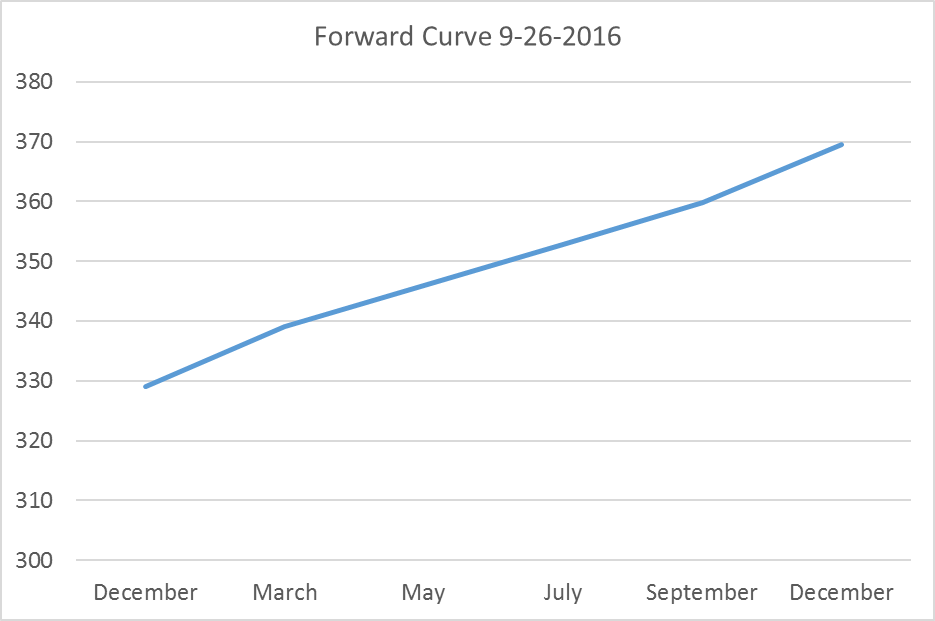
\includegraphics{Excel-files/PricesSpaceTime/forward-curves_files/image001.png}
\caption{Figure 1. Forward Curve on 9-26-2016}
\end{figure}

The reason that the forward curve represents return to storage is that
it shows how much extra money can be made by storing to a later date,
rather than selling in the cash `spot' market today. December corn is
worth 330 cents per bushel and March corn is worth 340 cents per bushel,
then you can make an extra 10 cents per bushel by selling the March
futures and selling into the cash market later.

In figure 2, the returns to storage per month are plotted. For example,
the we said that the return to storage between December and March is 10
cents per bushel. Since there are 2 months between December and March,
the per month return to storage is \(10/2 = 5\) cents per bushel. The
market is offering farmers and other holders of stocks 5 cents per month
to store grain between December and March.

\begin{figure}[htbp]
\centering
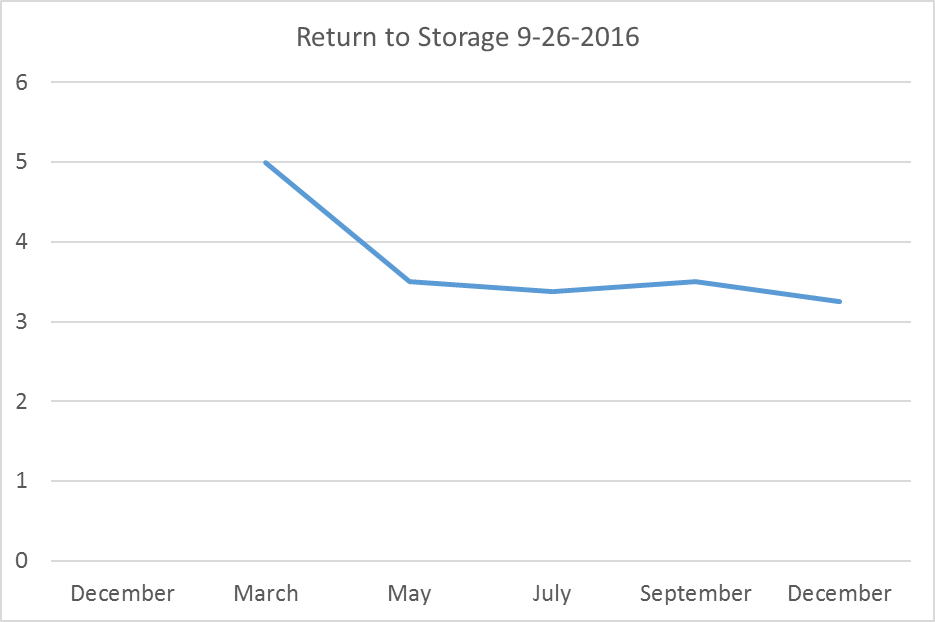
\includegraphics{Excel-files/PricesSpaceTime/forward-curves_files/image003.png}
\caption{Figure 2. Returns to Storage Per Month Implied by the Forward
Curve}
\end{figure}

What kind of market environment would produce such a result?

When stocks are plentiful the market offers a premium to those who are
willing to keep grain off the market for awhile. This prevents prices
from plunging too much right after a big harvest, since many choose to
wait for better prices later in the marketing year. Also, since these
price relationships are `discovered' and change every day, if it turns
out grain is coming onto the market too fast or too slowly, the return
to storage changes to alter the incentives so that supply and demand can
remain in equilibrium throughout the whole marketing year even though we
only harvest once per year (in North America).

This kind of market environment is sometimes called a \emph{carry
market} or sometimes it is said that the market is \emph{in full carry}.
This means that the market is offering returns to storage that covers
the cost to rent warehouse space, insure, and finance storing grain in
until a later date. The year of 2016 is certainly a full carry market.
Record production and a high forecast of ending stocks make this the
classic market environment where returns to storage would be positive.

As another example, the forward curve and returns to storage are shown
for 2015 in figures 3 and 4.

\begin{figure}[htbp]
\centering
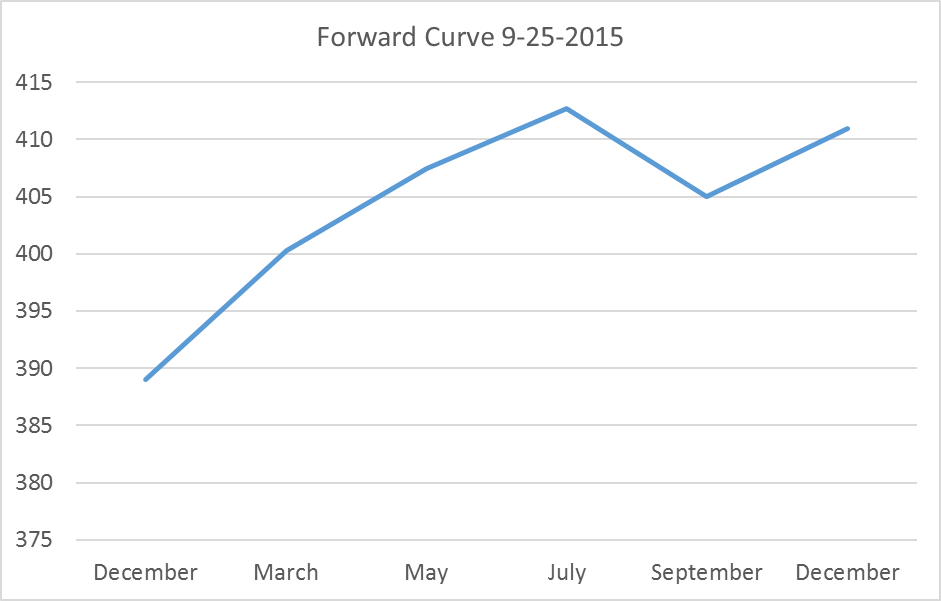
\includegraphics{Excel-files/PricesSpaceTime/forward-curves_files/image005.png}
\caption{Figure 3. Forward Curve on 9-25-2015}
\end{figure}

\begin{figure}[htbp]
\centering
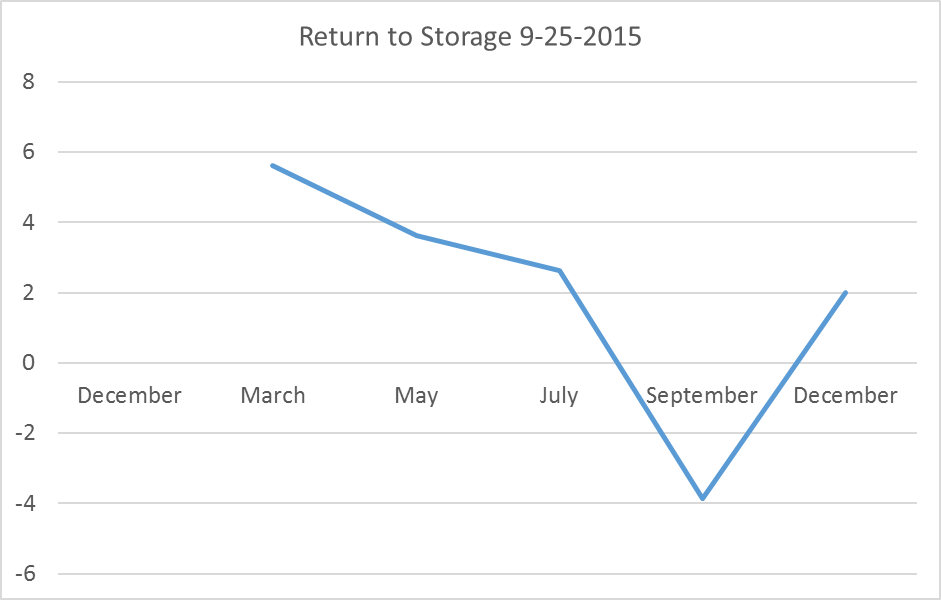
\includegraphics{Excel-files/PricesSpaceTime/forward-curves_files/image007.png}
\caption{Figure 4. Returns to Storage Per Month Implied by the Forward
Curve}
\end{figure}

This example illustrates a phenomenon that often occurs. Here we saw
that the forward curve is upward sloped until September. Then it
flattens and returns to storage go away. This makes sense because in
September we begin to see some of the next year's crop come onto the
market. So in 2015, the market was basically asking farmers to keep
storing through July, but no longer. Anyone planning to hold grain from
July to September and beyond could expect to lose as much as 4 cents per
month.

\section{A Decreasing Forward Curve}\label{a-decreasing-forward-curve}

Next we will consider a year that was characterized by a decreasing
forward curve. You will recall that 2012 was a significant drought year
that resulted in poor yields, high prices, and low forecasted ending
stocks for the marketing year. In this kind of market environment, where
supplies are tight, the forward curve tends to be downward sloped. The
implication of this is that anyone who decides to hold grain will lose
money because it is worth more today than it is tomorrow. The market is
incentivising everyone to bring grain onto the market.

We will look at the forward curve and return to storage in steps for
2012. On 4-13-2-12 the forward curve and returns to storage per month
are as shown in figure 5 and 6. This is in the spring, before the
drought has happened.

\begin{figure}[htbp]
\centering
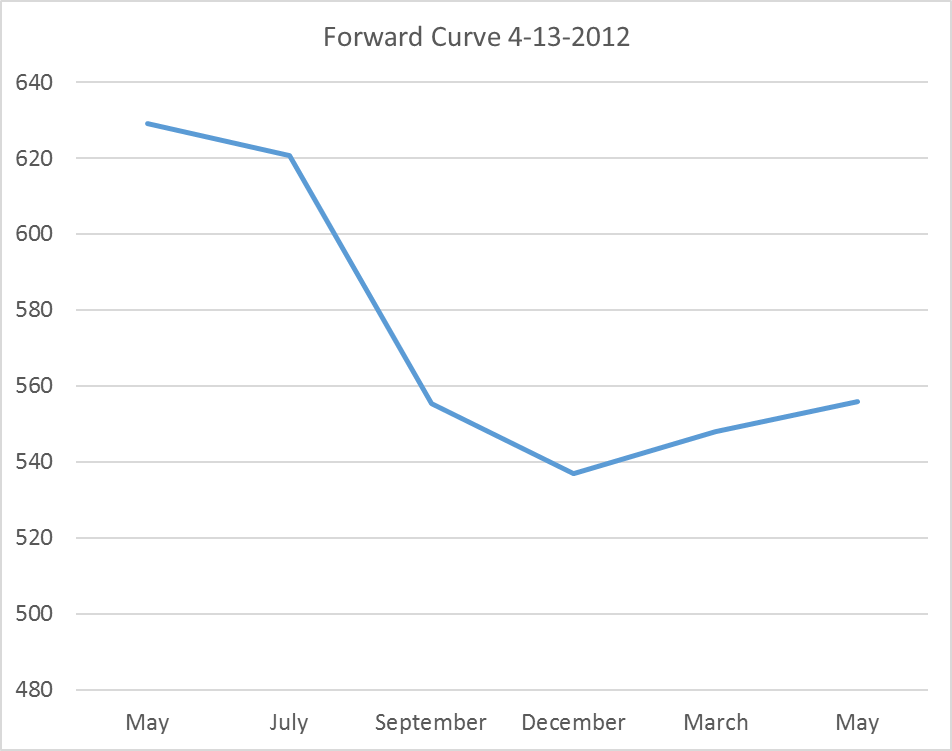
\includegraphics{Excel-files/PricesSpaceTime/forward-curves_files/image009.png}
\caption{Figure 5. Forward Curve on 4-13-2012}
\end{figure}

\begin{figure}[htbp]
\centering
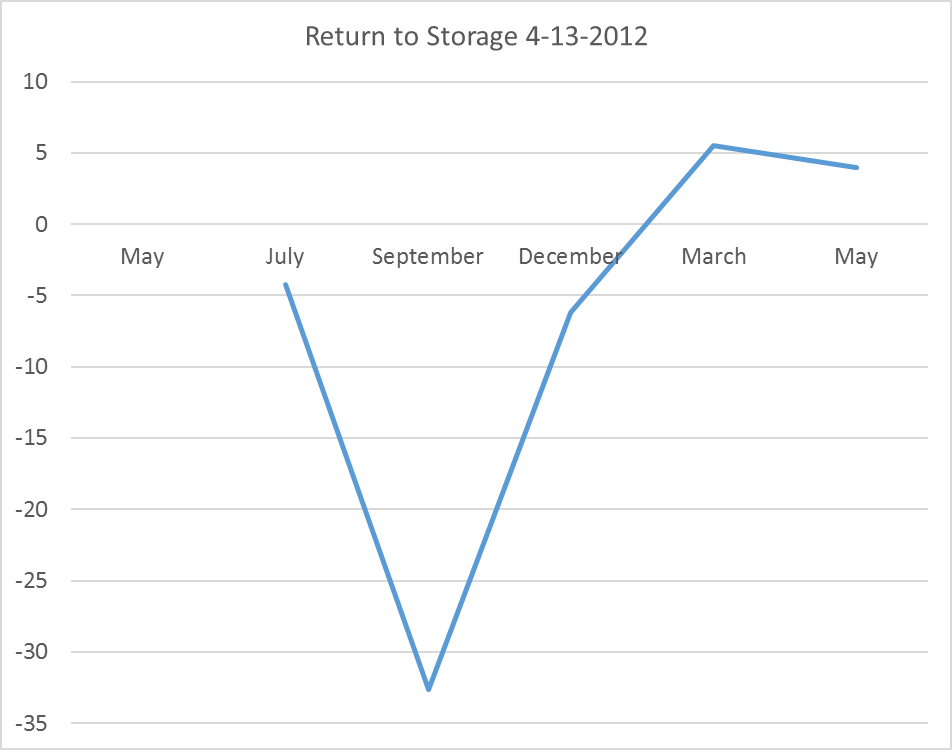
\includegraphics{Excel-files/PricesSpaceTime/forward-curves_files/image011.png}
\caption{Figure 6. Returns to Storage Per Month Implied by the Forward
Curve}
\end{figure}

In this case, supplies were already tight going into 2012. The forward
curve is downward sloped, also called \emph{inverted} or
\emph{backwardated}. So returns to storage are negative, as shown in
Figure 6 through the summer of 2012, even before we had the drought
realized. However, it is apparent from the forward curve that as of
4-13-2012, the market `thought' that the 2012 harvest would be good,
because price levels drop substantially in the September and December
contract, and the return to storage between December 2012 and March 2013
is positive on 4-13-2012.

Next, lets look at the forward curve and return to storage on 8-01-2012.
By August 1, it is clear that we are in the midst of a major drought,
yields will be low, and ending stocks for the coming marketing year will
be low as well.

Now, the forward curve is downward sloped and returns to storage are for
the entire marketing year until the next harvest, in 2013, is expected.
On 4-13-2012, the market was offering about 5 cents per month to store
from December 2012 to March 2013, by 8-01-2012, the return to storage
between the same time period was about -1 cent.

\begin{figure}[htbp]
\centering
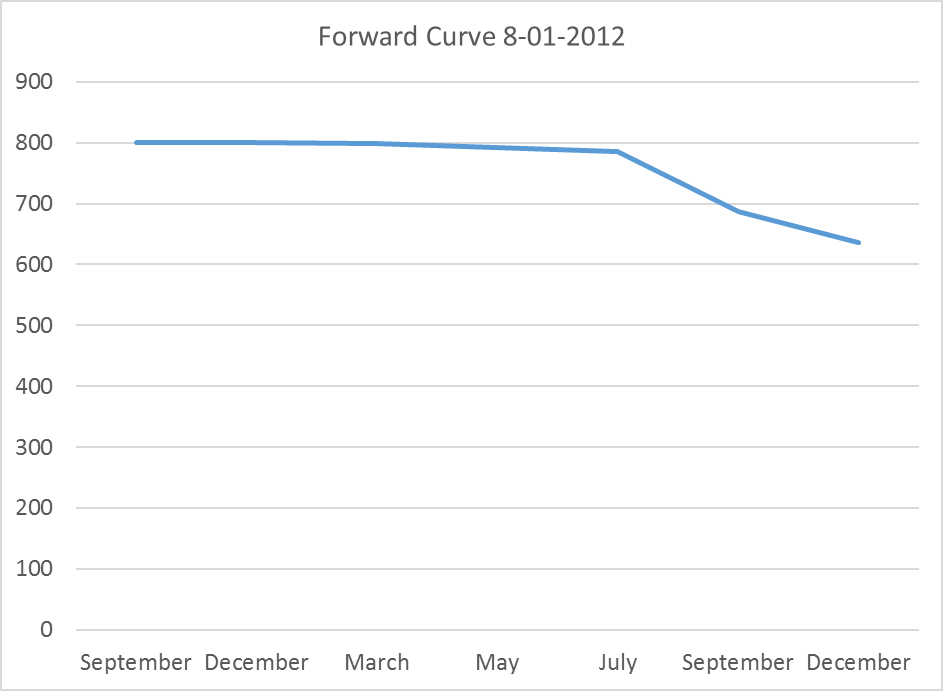
\includegraphics{Excel-files/PricesSpaceTime/forward-curves_files/image013.png}
\caption{Figure 7. Forward Curve on 8-01-2012}
\end{figure}

\begin{figure}[htbp]
\centering
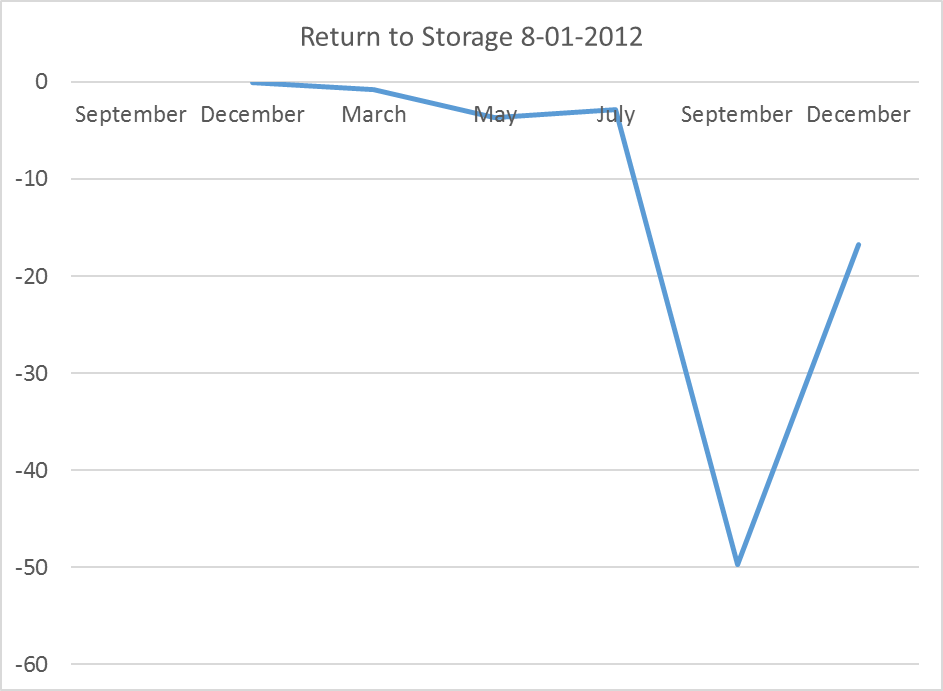
\includegraphics{Excel-files/PricesSpaceTime/forward-curves_files/image015.png}
\caption{Figure 8. Returns to Storage Per Month Implied by the Forward
Curve}
\end{figure}

Now, just to illustrate how the forward curve changed between August and
December 2012, the time in which harvest occurred and we learned exactly
how bad yields turned out to be, we show the forward curve and returns
to storage on 12-03-2012 in figures 9 and 10.

\begin{figure}[htbp]
\centering
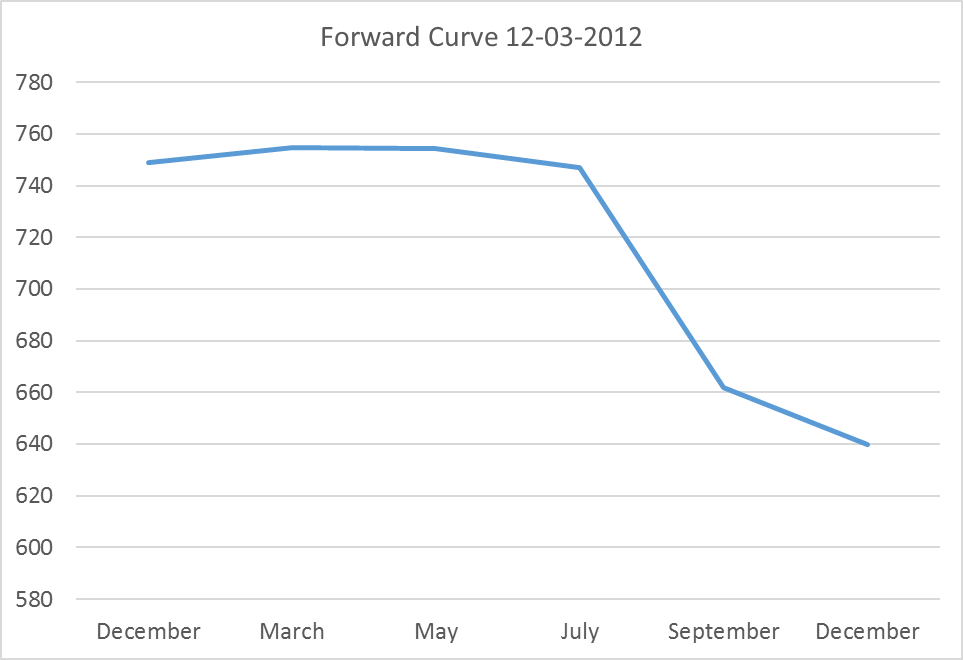
\includegraphics{Excel-files/PricesSpaceTime/forward-curves_files/image017.png}
\caption{Figure 9. Forward Curve on 12-03-2012}
\end{figure}

\begin{figure}[htbp]
\centering
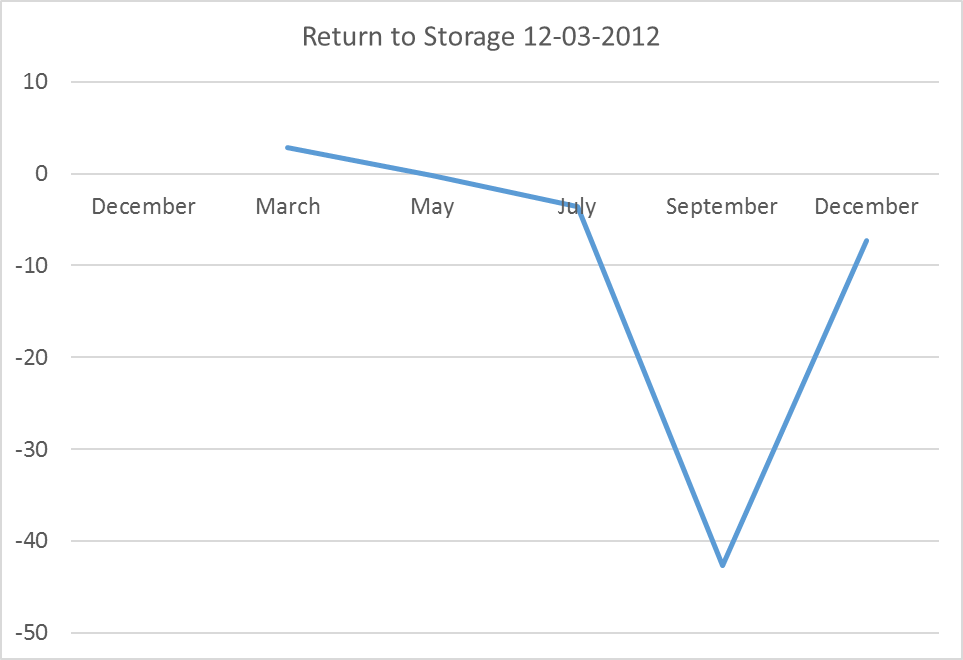
\includegraphics{Excel-files/PricesSpaceTime/forward-curves_files/image019.png}
\caption{Figure 10. Returns to Storage Per Month Implied by the Forward
Curve}
\end{figure}

\section{Calendar Spreads}\label{calendar-spreads}

The prior discussion has viewed the forward curve and returns to storage
from the perspective of a farmer or other who holds physical stocks of
grain. Speculators watch the price spread between futures contracts and
trade them to bet on whether or not returns to storage will increase or
decrease. These kinds of spreads are called \emph{Calendar Spreads} and
they are done by performing the following type of trade.

\subsection{Bullish}\label{bullish}

Buy: Dec 2016, Sell: March 2017

Then you are betting that prices in general will go up, but the nearby
will go up more than the deferred contracts. Any information event that
suggests supplies will become tighter should make prices go up in
general, and should reduce the incentive to store. Thus, making this a
profitable calendar spread trade.

\subsection{Bearish}\label{bearish}

Sell: Dec 2016, Buy: March 2017

The opposite logic is at work here. You are betting that prices will go
down in general, but that the nearby will go down more than the deferred
contracts. Any information that suggests supplies will become more
plentiful should make prices go down in general, and should increase
incentives to store. Thus making the bearish calendar spread profitable.

\section{Price Variation Over Space}\label{price-variation-over-space}

Most of our time in this course has focused on what impacts futures
prices for commodities. However, a futures price represent the expected
future price of the commodity in a very specific location - the
locations that are `regular' for delivery. A location that is regular
for delivery is a location that is designated by the commodity exchange
where stocks of a commodity represented by a futures contract may be
delivered in fulfillment of the contract. This is where the spot, or
cash, price must come together, or converge, with the futures price.

\begin{figure}[htbp]
\centering
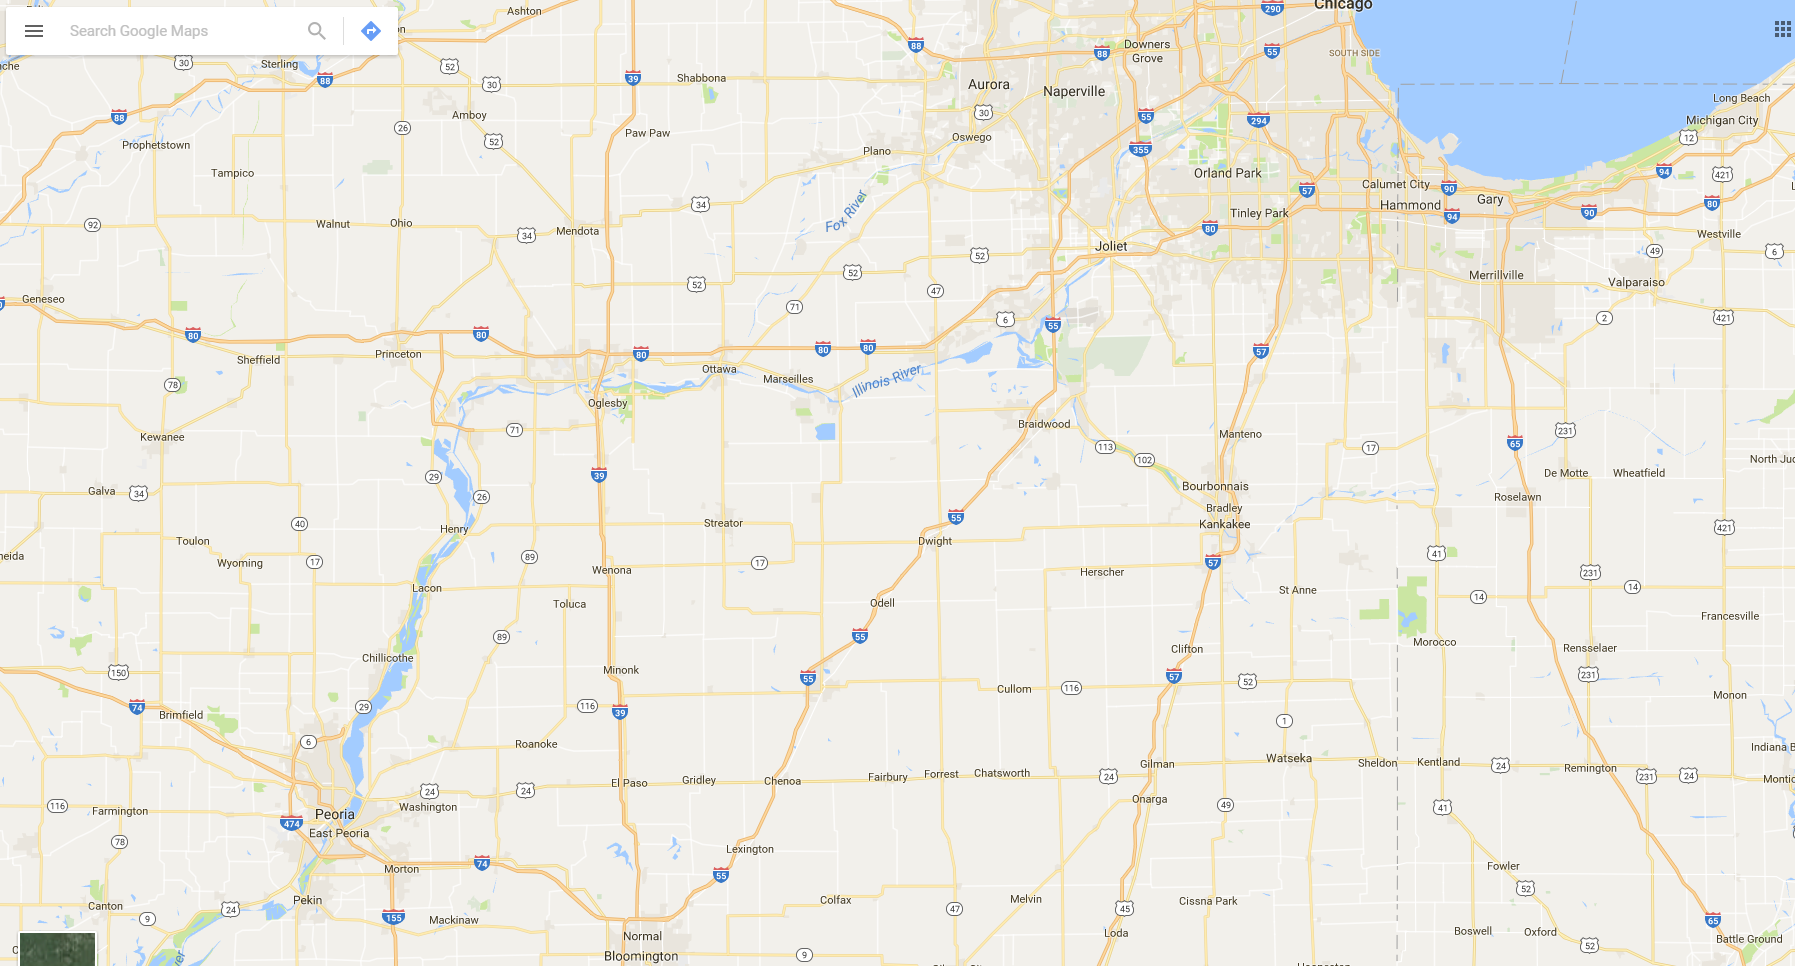
\includegraphics{images/IL-River.png}
\caption{Figure 11. Delivery Locations for Corn and Soybeans are Mostly
Along the Illinois River Between Chicago and Peoria, IL}
\end{figure}

(Source \href{https://www.google.com/maps}{Google Maps})

\begin{figure}[htbp]
\centering
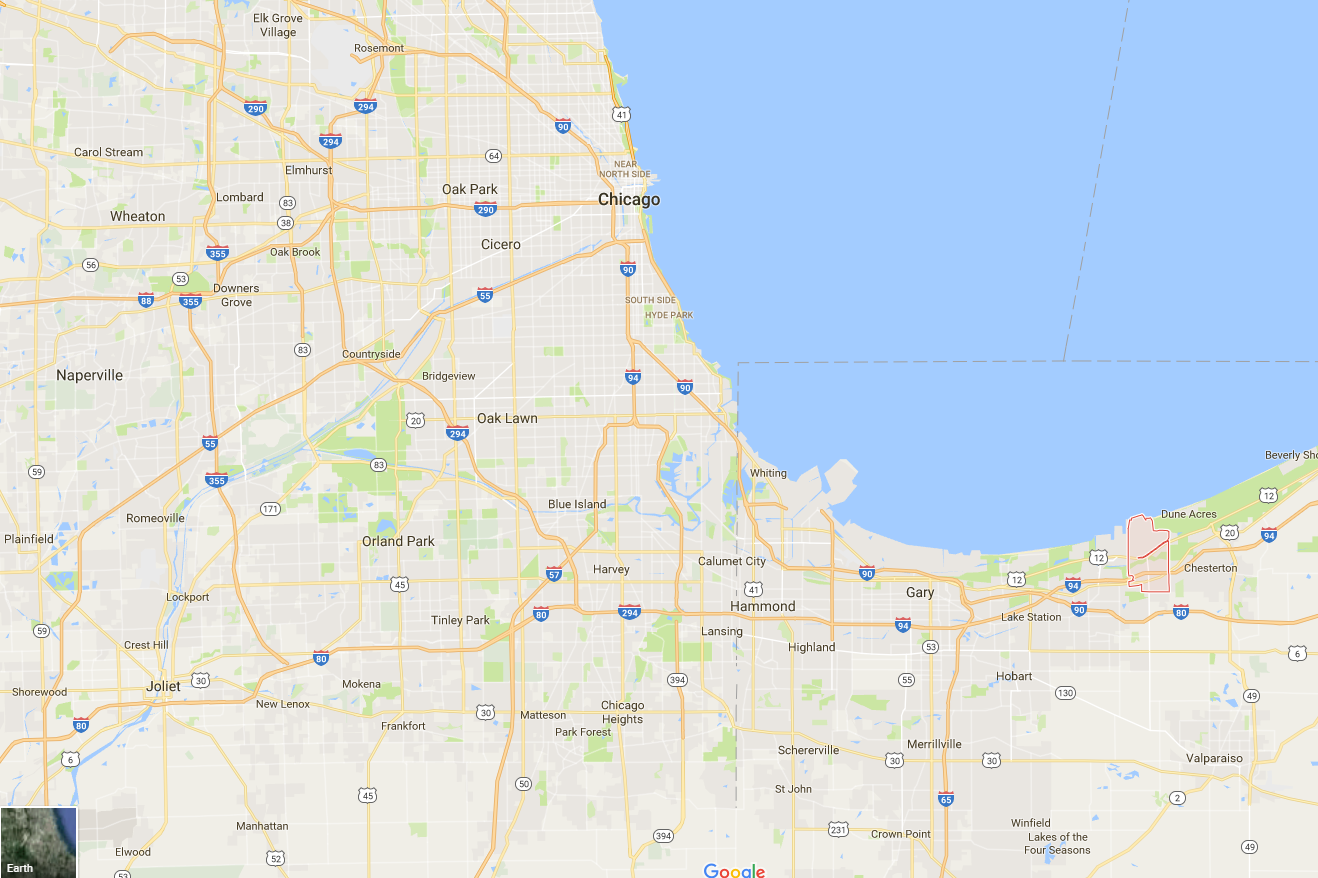
\includegraphics{images/Burns-Harbor.png}
\caption{Figure 12. Delvery Location at Burns Harbor, IN}
\end{figure}

(Source
\href{https://www.google.com/maps/place/Burns+Harbor,+IN/@41.740398,-87.7248706,10.5z/data=!4m5!3m4!1s0x8811bc3712ab828d:0x98301a46014d10b5!8m2!3d41.6258708!4d-87.1333676}{Google
Maps})

Since the price of the futures contract is represents the expected
future price only at these locations (technically whichever is cheapest
to deliver) then the degree to which the futures price is indicative of
the expected future spot price at locations far from Northern Illinois
can vary.

Throughout the rural U.S., grain elevators, ethanol plants, soybean
crushers, feed yards and biodeisel manufacturers dot the landscape every
few miles. These entities buy essentially all of the grain and oilseed
crop that is not used on-farm for livestock feeding. They post bids to
buy every day they are open. They offer to buy as a cash sale, or on
forward contract for delivery one to three months ahead. In the case of
the forward contract, the farmer will go in to the elevator and sign a
contract to deliver a specific number of bushels within a specified
window of time. Usually, the prices quoted by grain elevators and other
prices is relative to the futures contract price, or basis.

In figure 13 the elevators around Champiagn, IL are shown.

\begin{figure}[htbp]
\centering
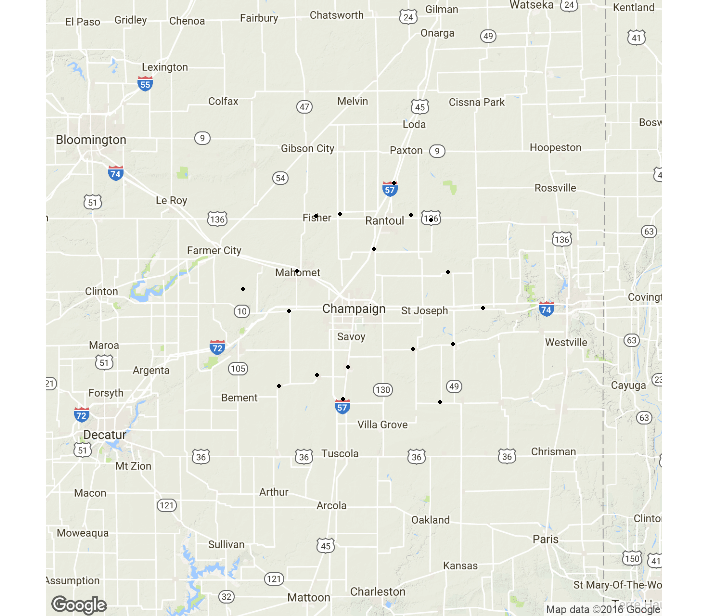
\includegraphics{images/Champaign-Elevators.png}
\caption{Figure 13. Elevators Around Champaign, IL}
\end{figure}

Depending on how far the location is from the Illinois river, this
difference may be large, but still the futures price is the reference
point. The basis is often quoted as `over' or `under' the futures price.
For example, an elevator might post bids to buy for \(-27\) cents. This
means \(27\) cents under the futures price. A bid of \(31\) would be
read as \(31\) cents over the futures price.

\section{Definition of Basis}\label{definition-of-basis}

Basis is always defined as Spot Price minus Futures price.

\[Basis = Spot - Futures\]

Basis reflects the price differential over space relative to the futures
price. Basis is influenced by

\begin{itemize}
\tightlist
\item
  Transportation Costs
\item
  Local Supply and Demand Conditions
\item
  Interest and Storage Charges (this reflects that there is also a small
  time component as well as spatial)
\item
  Other Handling, Shipping and other Costs
\end{itemize}

Transportation costs are built into basis because large users of grain
are not necessarily located in large production region. E.g., cattle
feed yards in Western Kansas and Nebraska; Chickens in the South; and
Hogs in North Carolina. Grain is shipped by rail and/or truck to
locations across the country. Areas of grain surplus generally have a
negative basis, the spot price is less than the futures. Areas of grain
deficit generally have a positive basis, the spot price is greater than
the futures.

Local supply and demand conditions are also important. Occasionally,
there will be localized production problems. The biggest recent example
comes from the demand side, however. The expansion in ethanol production
in the U.S. was felt greatest in Iowa. As literally billions of gallons
of capacity in ethanol production came online in Iowa, the corn basis
was affected. With additional large consumers of corn located throughout
Iowa, there was more localized demand for corn. The ethanol plants and
grain elevators had increased localized competition, and local basis
bids started to rise between 2005 and 2010.

\section{Terminology}\label{terminology}

Farmers and grain handlers alike watch the basis closely, so discussion
of changes in the basis is common. When the basis is increasing, in most
cases that means becoming `less negative', we say the basis is
\textbf{stregthening}. When the basis is decreasing, or becoming `more
negative', we say the basis is \textbf{weakening}.

\chapter{Balance Sheet Analysis}\label{balance-sheet-analysis}

Fundamental analysis is an assessment of price based on underlying
supply and demand factors. Focusing on changes in the relationship
between supply and demand allows one to calibrate an informed opinion of
the value of the commodity. The main role of the market is to find the
value at which supply equals demand - or in other words, the value that
`clears the market'. The estimated `fundamental value' is simply a
forecast, or expectation of, the market clearing price. The goal of any
forecasting exercise is to compare the forecast (estimated fundamental
value) to the current market price and make decisions accordingly.

\begin{quote}
Bullish: \texttt{Forecast\ \textgreater{}\ Price}\\
Bearish: \texttt{Forecast\ \textless{}\ Price}
\end{quote}

If your forecast is above the current market price, that is bullish
because your forecast implies the market is undervaluing the commodity -
an opportunity to buy low and sell high! If your forecast is below the
current market price, that is bearish because your forecast implies the
market is overvaluing the commodity - an opportunity to sell high and
buy low! This, of course, only works if your forecast is correct, that
is, the market eventually agrees and moves into line with your forecast.

\section{Supply and Demand}\label{supply-and-demand}

Conducing fundamental analyses involves taking into account all the
factors that determine supply, demand, and ultimately, prices. For grain
markets there are basically two supply models to keep in mind:
preplanting and post planting. Below we display both.

\begin{figure}[htbp]
\centering
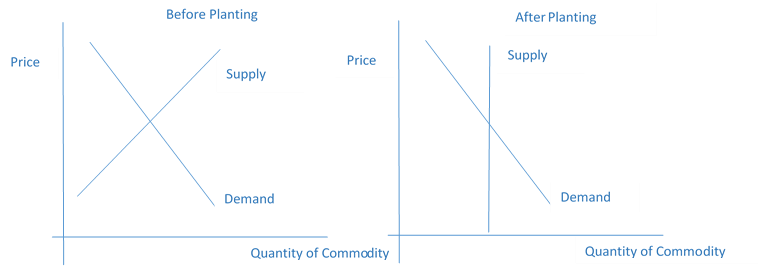
\includegraphics{images/Ch3.1.png}
\caption{Figure 1. Supply and Demand Model of a Commodity Before and
After Planting}
\end{figure}

The intuition here is simply that before planting, the final supply for
the crop can be affected by farmers changing their intentions about how
many acres to plant. Once the crop has been planted, supply is
essentially fixed, except for the uncertainty that remains due to
realized yields. To summarize, things that affect the supply of a
commodity are outlined below.

\textbf{Supply is Affected by:}

\begin{itemize}
\tightlist
\item
  Acreage

  \begin{itemize}
  \tightlist
  \item
    Prices of crops competing for acreage
  \item
    Pre-Plant Weather
  \end{itemize}
\item
  Yield

  \begin{itemize}
  \tightlist
  \item
    Post-Plant Weather
  \end{itemize}
\item
  Government Policies
\end{itemize}

\begin{description}
\item[Acreage]
Before planting, farmers plan how much acreage to devote to each
commodity, thus determining the baseline expected production level.
Before summer weather is revealed, expected production is simply
\texttt{Acreage\ X\ Trend\ Yield}. In the Corn Belt, where planting
decisions amount to deciding how to divide acres between corn and
soybeans, their relative prices play a large role in the farmer's
decision. If futures prices indicate planting soybeans will be more
profitable than planting corn, farmers will plan to devote more acres
than usual to soybeans, for example. Weather can be an important
determinant of acreage decisions as well. The most ardent planting
intentions of a farmer can be derailed by persistent wet weather. An
unusually rainy planting season can reduce planted acres from
intentions. Before the crop is actually in the ground, the supply of
grain is relatively elastic.
\item[Yield]
After the crop is planted supply is quite inelastic, but there is still
considerable uncertainty related to how much the crop will yield; this
is largely determined by weather during the growing season.
\item[Government Policies]
The government has been heavily involved in Agriculture in the United
States since the great depression of the 1930's. There have been
programs that guarantee a minimum price, programs that guarantee minimum
revenue, and various incarnations of crop insurance programs.
Occasionally these favor the production of one type of crop over
another. When this happens, farmers predictably respond by planting more
of the crop treated more favorably by the program.
\end{description}

\textbf{Demand is Affected by:}

\begin{itemize}
\tightlist
\item
  Consumer Income
\item
  Exchange Rates
\end{itemize}

\begin{description}
\item[Consumer Income]
This one is straight from economics 101. When people have more money,
they will spend it on goods. This means increased demand for commodities
and their derived products. This includes foreign income, since exports
are a big component of demand for commodities in the United States.
Rising incomes usually means rising consumption of meat, which increases
the demand for commodities like corn, soybeans, and even wheat that are
used as animal feed.
\item[Exchange Rates]
Exchange rates also affect demand through their influence on exports.
For example, if the U.S. dollar is weak, then consumers in other
countries can buy dollars cheaply - giving them more purchasing power
for goods denominated in dollars.
\end{description}

\section{Balance Sheet}\label{balance-sheet}

Most fundamental analyses rely on maintaining balance sheets of a
commodity for a country, region, or the world. The approach is to
maintain a careful accounting of how much supply exists and how much of
the commodity has been used. Then through various means we will explore
later, one arrives at a price that is expected to ration remaining
supplies across competing uses.

\subsection{The Marketing Year and Balance Sheet Forecasting
Schedule}\label{the-marketing-year-and-balance-sheet-forecasting-schedule}

Balance sheet analysis is often organized by marketing year. Since
production happens once per year, the marketing year is defined to begin
in the first month the commodity is harvested and ends with the
following year's harvest. The table below makes note the month on which
marketing years begin for several crops.

\begin{longtable}[]{@{}ll@{}}
\caption{Table 1. Beginning of Marketing Year by Crop. (Source
\href{http://www.nass.usda.gov/Publications/National_Crop_Progress/}{NASS
Timetables})}\tabularnewline
\toprule
Crop & Beginning of Marketing Year - First Month of
Harvest\tabularnewline
\midrule
\endfirsthead
\toprule
Crop & Beginning of Marketing Year - First Month of
Harvest\tabularnewline
\midrule
\endhead
Corn & September\tabularnewline
Soybeans & September\tabularnewline
Spring Wheat (Chicago) & August\tabularnewline
Winter Wheat (KC) & July\tabularnewline
\bottomrule
\end{longtable}

Forecasting supply and demand for any given marketing year begins well
before harvest - nearly a year in advance, in fact. Table 2 below
follows the typical forecasting schedule with the 2016/2017 marketing
year. Note that is for the marketing year that begins with harvest in
September of 2016.

\begin{longtable}[]{@{}ll@{}}
\caption{Table 2: Forecasting Calendar for 2016/2017 Marketing
Year}\tabularnewline
\toprule
\begin{minipage}[b]{0.19\columnwidth}\raggedright\strut
Timeline\strut
\end{minipage} & \begin{minipage}[b]{0.75\columnwidth}\raggedright\strut
Forecasting Focus\strut
\end{minipage}\tabularnewline
\midrule
\endfirsthead
\toprule
\begin{minipage}[b]{0.19\columnwidth}\raggedright\strut
Timeline\strut
\end{minipage} & \begin{minipage}[b]{0.75\columnwidth}\raggedright\strut
Forecasting Focus\strut
\end{minipage}\tabularnewline
\midrule
\endhead
\begin{minipage}[t]{0.19\columnwidth}\raggedright\strut
Fall 2015\strut
\end{minipage} & \begin{minipage}[t]{0.75\columnwidth}\raggedright\strut
The first forecasts of supply and use based on , \emph{trend forecasts},
\emph{recent history}, \emph{economic relationships}\strut
\end{minipage}\tabularnewline
\begin{minipage}[t]{0.19\columnwidth}\raggedright\strut
Spring 2016\strut
\end{minipage} & \begin{minipage}[t]{0.75\columnwidth}\raggedright\strut
Update supply forecasts based on USDA acreage surveys.\strut
\end{minipage}\tabularnewline
\begin{minipage}[t]{0.19\columnwidth}\raggedright\strut
Summer 2016\strut
\end{minipage} & \begin{minipage}[t]{0.75\columnwidth}\raggedright\strut
Update supply forecasts based on weather and USDA crop and stocks
reports\strut
\end{minipage}\tabularnewline
\begin{minipage}[t]{0.19\columnwidth}\raggedright\strut
Fall 2016\strut
\end{minipage} & \begin{minipage}[t]{0.75\columnwidth}\raggedright\strut
Update supply forecasts as yield uncertainty is resolved through harvest
reports and USDA production reports\strut
\end{minipage}\tabularnewline
\begin{minipage}[t]{0.19\columnwidth}\raggedright\strut
- Summer 2016\strut
\end{minipage} & \begin{minipage}[t]{0.75\columnwidth}\raggedright\strut
Continue to update supply forecasts based on USDA production revisions,
southern hemisphere production, stocks, and use reports.\strut
\end{minipage}\tabularnewline
\bottomrule
\end{longtable}

\begin{quote}
\chapter{Southern Hemisphere
Production}\label{southern-hemisphere-production}

Production of corn, soybeans, and other commodities in the southern
hemisphere (most notably in Brazil and Argintina) has grown rapidly over
the last ten to fifteen years, and has impacted global commodity markets
tremendously. Since southern hemisphere production occurs in the middle
of marketing years organized by northern hemisphere harvest, there is an
uncertain additional supply that must be forecast and updated to keep an
accurate global balance sheet.
\end{quote}

\subsection{Uncertainty}\label{uncertainty}

Even careful accounting of supply and demand factors that make up the
balance sheet leaves a tremendous amount of uncertainty in the market.
Demand can be difficult to forecast, and can sometimes change
dramatically. The USDA keeps careful track of stocks, but we only get
stocks estimates once a quarter. Between \emph{Grain Stocks} reports
there is always a great deal of speculation as to the pace of
consumption and whether we are eating into stocks at a faster or slower
pace than expected. Analysts talk about whether the market is on pace to
achieve the forecast level of ethanol crush, soybean crush, or exports.
Surprises in any of these components can lead to rapid corrections in
the commodity markets.

\subsection{Balance Sheet Format}\label{balance-sheet-format}

Here we discuss the common format balance sheets for any commodity have
in common. Then we talk about the components of specific balance sheets
for corn and soybeans.

\begin{longtable}[]{@{}ll@{}}
\caption{Table 3. Balance Sheet for a General Commodity}\tabularnewline
\toprule
Stocks and Use &\tabularnewline
\midrule
\endfirsthead
\toprule
Stocks and Use &\tabularnewline
\midrule
\endhead
Beginning Stocks &\tabularnewline
+ Production &\tabularnewline
+ Imports &\tabularnewline
\textbf{= Total Supply} &\tabularnewline
Domestic Consumption &\tabularnewline
+ Exports &\tabularnewline
+ Residual &\tabularnewline
\textbf{= Total Consumption (Use)} &\tabularnewline
\textbf{Ending Stocks = Total Supply - Total Consumption}
&\tabularnewline
\bottomrule
\end{longtable}

Since the USDA makes regular reports on the balance sheet for
commodities (the WASDE reports described in Chapter 2), most conducing
private analyses with balance sheets use the USDA categories so that the
USDA estimates can be taken as a benchmark. The supply side (Stocks) is
relatively straightforward. Total stocks for the marketing year will be
beginning stocks, the portion of last year's stocks that were not used
up during the previous marketing year, plus this year's production, plus
any imports of the commodity. Summing these three reveals the total
amount of the commodity available for use during the marketing year.

\begin{itemize}
\tightlist
\item
  Beginning Stocks: Some production from the previous year usually
  remains into the next crop season. Carryover stocks function as a
  buffer against current year yield uncertainty. For example, if
  carryover stocks are high and current year yield is expected to be
  below trend, the market price may fall in response but modestly.
  However, if carryover stocks are low - resulting from several years of
  below trend production and strong demand - then an expected yield
  below trend will likely cause a volatile rise in prices.
\end{itemize}

: Table 4. August 2016 USDA WASDE Balance Sheet for Corn

\begin{tabular}{l|l|l|l|l}
\hline
Corn & Marketing Year 2014/2015 & Marketing Year 2015/2016 Est. & Marketing Year 2016/2017 July Projection & Marketing Year 2016/2017 August Projection\\
\hline
**Million Acres** &  &  &  & \\
\hline
Area Planted & 90.6 & 88 & 94.1 * & 94.1\\
\hline
Area Harvested & 83.1 & 80.7 & 86.6 * & 86.6\\
\hline
**Bushels** &  &  &  & \\
\hline
Yield per Harvested Acre & 171 & 168.4 & 168.0 * & 175.1\\
\hline
**Million Bushels** &  &  &  & \\
\hline
Beginning Stocks & 1232 & 1731 & 1701 & 1706\\
\hline
Production & 14216 & 13601 & 14540 & 15153\\
\hline
Imports & 32 & 65 & 40 & 50\\
\hline
**Supply, Total** & **15479** & **15397** & **16281** & **16909**\\
\hline
Feed and Residual & 5314 & 5200 & 5500 & 5675\\
\hline
Food, Seed \& Industrial & 6567 & 6567 & 6650 & 6650\\
\hline
*Ethanol \& by-products* & *5200* & *5200* & *5275* & *5275*\\
\hline
Domestic, Total & 11881 & 11767 & 12150 & 12325\\
\hline
Exports & 1867 & 1925 & 2050 & 2175\\
\hline
**Use, Total** & **13748** & **13692** & **14200** & **14500**\\
\hline
Ending Stocks & 1731 & 1706 & 2081 & 2409\\
\hline
**Avg. Farm Price (\$/bu)** & **3.7** & **3.55 - 3.65** & **3.10 - 3.70** & **2.85 - 3.45**\\
\hline
\end{tabular}

(source: August 2016 USDA
\href{http://usda.mannlib.cornell.edu/MannUsda/viewDocumentInfo.do?documentID=1194}{WASDE
Report} )

The balance sheet for corn follows the same generic patter, but we can
be a bit more specific with the use categories since we know what the
major use categories are for any given commodity. The use components are
as follows:

\begin{itemize}
\tightlist
\item
  Feed and Residual: A large portion of the corn crop is used as feed
  for livestock (cattle, pigs, poultry).
\item
  Food, Seed, and Industrial: Corn is used to make tortilla chips, high
  fructose corn syrup, edible oil and other food items. A portion of the
  crop is grown specifically as seed for the next years crop. There are
  some industrial uses for components of processed corn. Those are
  grouped in this category as well.
\item
  Ethanol production also demands a significant amount of corn, so much
  that it gets its own line in the balance sheet. Note, however, that it
  is technically part of the Food, Seed, and Industrial category.
\item
  The final use category is export. Corn grown in the United States is
  consumed around the globe, and strength or weakness in the export
  market is a carefully component of demand.
\end{itemize}

: Table 5. August 2016 USDA WASDE Balance Sheet for Soybeans

\begin{tabular}{l|l|l|l|l}
\hline
Soybeans & Marketing Year 2014/2015 & Marketing Year 2015/2016 Est. & Marketing Year 2016/2017 July Projection & Marketing Year 2016/2017 August Projection\\
\hline
**Million Acres** &  &  &  & \\
\hline
Area Planted & 83.3 & 82.7 & 83.7* & 83.7\\
\hline
Area Harvested & 82.6 & 81.8 & 83* & 83\\
\hline
**Bushels** &  &  &  & \\
\hline
Yield per Harvested Acre & 47.5 & 48 & 48.9* & 50.6\\
\hline
**Million Bushels** &  &  &  & \\
\hline
Beginning Stocks & 92 & 191 & 255 & 195\\
\hline
Production & 3927 & 3929 & 4060 & 4201\\
\hline
Imports & 33 & 25 & 30 & 30\\
\hline
**Supply, Total** & **4052** & **4145** & **4346** & **4426**\\
\hline
Crushings & 1873 & 1900 & 1940 & 1950\\
\hline
Exports & 1842 & 1880 & 1950 & 1985\\
\hline
Seed & 96 & 97 & 95 & 95\\
\hline
Residual & 50 & 12 & 31 & 31\\
\hline
**Use, Total** & **3862** & **3889** & **4016** & **4061**\\
\hline
Ending Stocks & 191 & 255 & 330 & 365\\
\hline
**Avg. Farm Price (\$/bu)** & **10.1** & **8.95** & **8.35 - 9.85** & **8.30 - 9.80**\\
\hline
\end{tabular}

(source: August 2016 USDA
\href{http://usda.mannlib.cornell.edu/MannUsda/viewDocumentInfo.do?documentID=1194}{WASDE
Report} )

For soybeans, stocks are comprised of beginning stocks, production, and
imports, just as they were for the general balance sheet and the corn
balance sheet. The use side, contains items specific to soybeans:

\begin{itemize}
\tightlist
\item
  Crush: The amount of raw soybeans that are processed into soybean oil
  and soybean meal. Soybean oil is used predominately as edible oil; it
  also is used to make bio-diesel in modest quantities.
\item
  Food, Seed, and Industrial: We saw this category in the corn balance
  sheet. The definition remains the same.
\item
  Exports: The United States exports a large quantity of soybeans to
  global buyers.
\end{itemize}

\section{Coming up with a Price}\label{coming-up-with-a-price}

Balance sheet forecasting is definitely as much art as it is science. It
involves keeping track of the rate of use of commodities to see how much
a need there will be to ration late in the marketing year while waiting
on harvest and new supplies. One should intuitively see that the
forecasted ending stocks is a measure of scarcity of the commodity and
therefore should be negatively related to price (i.e., tight ending
stocks go along with high prices). One needs to pin down the exact
nature of this relationship in order to form a meaningful forecast of
price from a commodity balance sheet. We will discuss this process in
more detail in a later chapter.

\section{Readings}\label{readings-2}

\begin{description}
\item[\href{http://farmdocdaily.illinois.edu/2015/02/balance-sheet-projections-for-2015-16-corn-marketing-year.html}{Balance
Sheet Projections for the 2015-16 Corn Marketing Year}]
This \emph{farmdoc daily} article was written in February of 2015. This
is well before spring planting of corn and soybeans in the United
States. However, farmers during this time are actively planning for
planting season - prepping equipment, fertilizing and preparing ground,
and buying seed. Good lays out the groundwork for early forecasts of the
2015/2016 marketing year balance sheet. This article is published two
days before the February 2015 WASDE report, and Good provides context
upon which market expectations for the WASDE report can be based upon.

Good, D.
``\href{http://farmdocdaily.illinois.edu/2015/02/balance-sheet-projections-for-2015-16-corn-marketing-year.html}{Balance
Sheet Projections for the 2015-16 Corn Marketing Year}.'' \emph{farmdoc
daily} (5):23, Department of Agricultural and Consumer Economics,
University of Illinois at Urbana-Champaign, February 9, 2015.
\item[\href{http://farmdocdaily.illinois.edu/2015/04/projecting-2015-16-corn-balance-sheet.html}{Projecting
the 2015-16 Corn Balance Sheet and Price Implications}]
In this reading Good and Irwin break down the USDA's April 9th WASDE
report and offer their own projections that differ slightly from the
USDA's projection that came out a week earlier. Pay close attention to
why their price estimate is higher than the USDA's.

Good, D., and S. Irwin.
``\href{http://farmdocdaily.illinois.edu/2015/04/projecting-2015-16-corn-balance-sheet.html}{Projecting
the 2015-16 Corn Balance Sheet and Price Implications}.'' \emph{farmdoc
daily} (5):70, Department of Agricultural and Consumer Economics,
University of Illinois at Urbana-Champaign, April 16, 2015.
\end{description}

\section{Exercises}\label{exercises-2}

\begin{enumerate}
\def\labelenumi{\arabic{enumi}.}
\item
  Copy and paste the corn and soybeans balance sheets into a
  spreadsheet.

  \begin{itemize}
  \tightlist
  \item
    In the cell next to \textbf{= Total Supply}, manually add the cells
    needed to reproduce the \textbf{`=Total Supply'} number.
  \item
    in the cell next to \textbf{= Total Consumption}, manually add the
    cells needed to reproduce the \textbf{= Total Consumption} number.
  \end{itemize}
\item
  If you were making a forecast in July 2015 for the 2014/2015 marketing
  year balance sheet, which columns (if any) should remain fixed? I.e.,
  they are already determined and do not need to be forecast.
\item
  If you were making a forecast in July 2015 for the 2015/2016 marketing
  year balance sheet, which columns (if any) should remain fixed?
\end{enumerate}

\chapter{Price Reaction to USDA
Reports}\label{price-reaction-to-usda-reports}

Some of the USDA reports contain very sensitive market information
causing market prices to adjust rapidly to new information about supply
and demand. Access to the contents of a market sensitive report would
result in the ability to perform `insider trading' and obtain nearly
risk-less profits. This activity is illegal, and the USDA's NASS
prepares the reports under lock-down conditions where during the process
of finalizing estimates of the report's content, officials are locked in
a secure area and not allowed to leave until the report is made known to
the public.

This chapter explores some history related to the compilation and
release of USDA reports, discusses how release times have evolved over
time, indicates some particular report releases that are more likely to
cause large and rapid price adjustments, and demonstrates this with a
few charts of transactions prices pre- and post-release of particularly
interesting recent days.

\section{\texorpdfstring{History - ``The Great Data Leak of
1905''}{History - The Great Data Leak of 1905}}\label{history---the-great-data-leak-of-1905}

This abundance of care can be traced to a particular event in history.
The details of which are recounted in a historical publication by the
NASS.

\begin{figure}[htbp]
\centering
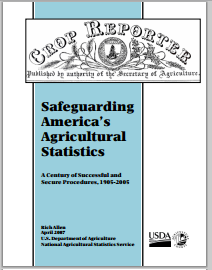
\includegraphics{images/NASS_History.png}
\caption{Figure 1: Safeguarding America's Agricultural Statistics: A
century of Successful and Secure Procedures}
\end{figure}

Source:
\href{pdf-readings/safegaurding-americas-agricultural-statistics.pdf}{NASS:
About Nass}

\begin{quote}
\section{Excerpt From Chapter 1}\label{excerpt-from-chapter-1}

The summary and release procedures for the USDA Bureau of Statistics'
reports in the early 1900s produced separate summary tabulations for
each data source available (up to six sources, in some cases)\ldots{} It
is also relevant that the release time for cotton reports in those years
was noon, Eastern Time, and that the commodity markets discontinued
trading for an hour starting at noon on release days. The original
procedures allowed the three people who had determined the final numbers
to go about their business, or even leave the building if they wished,
once a report's contents had been set.

In 1904 there were rumors about insider trading. As came to light later,
one of the three Bureau of Statistics people, E.S. Holmes, Jr., did have
an outside partner, a NewYork cotton trader named Louis Van Riper.
Shortly after an estimate was set, Holmes would meet Van Riper and tell
him what cotton estimate was going to be published. Van Riper would take
whatever market action would be most profitable based on the advance
information.

The scheme came to light following the cotton acreage report issued on
June 2, 1905. The three members met and adopted the state and national
figures to be published. After Holmes had sent his signal, one of the
other people who had worked on the report asked for reconsideration.
After further review, the figures to be published were revised. At that
point, the outside partner had already interpreted the original signal
and proceeded to place trades. The scheme came to light when Van Riper
charged in a telegram that a ``fraudulent'' report had been released. In
explaining why he thought this was a false report, he unwittingly
revealed that he had the information ahead of time. Evidently, Holmes'
outside partner had an overabundance of ego, but not a good balance of
common sense in going public with his story. \citep{history2007Nass}
\end{quote}

\section{Changing Report Release
Times}\label{changing-report-release-times}

Timing of report releases has important implications for the market
reaction as well. Figure 2 below provides a brief history of report
release times of major market sensitive reports.

\begin{figure}[htbp]
\centering
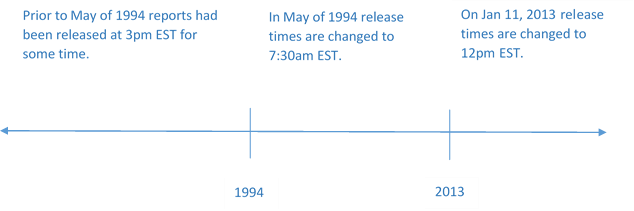
\includegraphics{images/NASS_release_timeline.png}
\caption{Figure 2: Timeline of Report Release Times}
\end{figure}

Prior to 1994 most market sensitive USDA reports were released at 3pm
EST. This made sense from the USDA workflow perspective because it
allowed the lock-down to be enacted during normal working hours,
minimizing disruption of the analysts' regular lives. By the early 90's
releasing the report at this time became unpopular with market
participants. By releasing the report late in the afternoon in the U.S.
futures markets in other parts of the world could trade the USDA numbers
overnight before the U.S. market had a chance to react. Therefore price
discovery after reports was essentially shifted from Chicago to other
major exchanges across the world.

In May of 1994, the USDA shifted the release time to 8:30am EST. This
meant the report was released during regular business hours in the U.S.
and just one hour before trading begins on the U.S. futures exchange.
While clearly preferable to market participants in the U.S. this moved
the USDA's lockup time to overnight hours \citep{history2007Nass}.

By 2011, presumably due to the ability to trade electronically with high
speed, there was a desire for the futures market to be open and actively
trading at the time USDA reports were released. In this case, the
futures exchange acted first, expanding trading hours to an earlier
market open. Eventually, since futures market participants wanted it,
and because came with the added benefit of moving the beginning of the
lockup period from late night to early morning, the USDA began releasing
most reports at 12pm EST on January 11, 2013.

\section{Price Reactions}\label{price-reactions}

Market prices react strongly to USDA reports when the reports inject
significant and unanticipated information into the market. Some reports
are more likely than others to produce fireworks in terms of market
price.

\begin{longtable}[]{@{}lll@{}}
\caption{Table 1: Reports most likely to cause significant movements in
market price}\tabularnewline
\toprule
\begin{minipage}[b]{0.11\columnwidth}\raggedright\strut
Report\strut
\end{minipage} & \begin{minipage}[b]{0.10\columnwidth}\raggedright\strut
Dates\strut
\end{minipage} & \begin{minipage}[b]{0.11\columnwidth}\raggedright\strut
Reason\strut
\end{minipage}\tabularnewline
\midrule
\endfirsthead
\toprule
\begin{minipage}[b]{0.11\columnwidth}\raggedright\strut
Report\strut
\end{minipage} & \begin{minipage}[b]{0.10\columnwidth}\raggedright\strut
Dates\strut
\end{minipage} & \begin{minipage}[b]{0.11\columnwidth}\raggedright\strut
Reason\strut
\end{minipage}\tabularnewline
\midrule
\endhead
\begin{minipage}[t]{0.11\columnwidth}\raggedright\strut
Grain Stocks\strut
\end{minipage} & \begin{minipage}[t]{0.10\columnwidth}\raggedright\strut
Quarterly\strut
\end{minipage} & \begin{minipage}[t]{0.11\columnwidth}\raggedright\strut
Information about scarcity or surplus of supplies\strut
\end{minipage}\tabularnewline
\begin{minipage}[t]{0.11\columnwidth}\raggedright\strut
Prospective Plantings\strut
\end{minipage} & \begin{minipage}[t]{0.10\columnwidth}\raggedright\strut
End of March\strut
\end{minipage} & \begin{minipage}[t]{0.11\columnwidth}\raggedright\strut
Acreage and therefore production estimates\strut
\end{minipage}\tabularnewline
\begin{minipage}[t]{0.11\columnwidth}\raggedright\strut
Planted Acres\strut
\end{minipage} & \begin{minipage}[t]{0.10\columnwidth}\raggedright\strut
End of June\strut
\end{minipage} & \begin{minipage}[t]{0.11\columnwidth}\raggedright\strut
Acreage and therefore production estimates\strut
\end{minipage}\tabularnewline
\begin{minipage}[t]{0.11\columnwidth}\raggedright\strut
WASDE\strut
\end{minipage} & \begin{minipage}[t]{0.10\columnwidth}\raggedright\strut
October\strut
\end{minipage} & \begin{minipage}[t]{0.11\columnwidth}\raggedright\strut
Some years the Oct report will contain significant revisions from
previous estimate\strut
\end{minipage}\tabularnewline
\begin{minipage}[t]{0.11\columnwidth}\raggedright\strut
WASDE\strut
\end{minipage} & \begin{minipage}[t]{0.10\columnwidth}\raggedright\strut
January\strut
\end{minipage} & \begin{minipage}[t]{0.11\columnwidth}\raggedright\strut
Final production estimate for the preceding harvest. Sometimes includes
and unanticipated revision\strut
\end{minipage}\tabularnewline
\begin{minipage}[t]{0.11\columnwidth}\raggedright\strut
Crop Progress Report\strut
\end{minipage} & \begin{minipage}[t]{0.10\columnwidth}\raggedright\strut
Weekly\strut
\end{minipage} & \begin{minipage}[t]{0.11\columnwidth}\raggedright\strut
Condition estimates. Only moves market prices if significant
deterioration associated with a drought or flood occurs\strut
\end{minipage}\tabularnewline
\bottomrule
\end{longtable}

\begin{description}
\item[Grain stocks]
Estimates only come out quarterly. Since the information about whether
we have a scarcity or surplus is a primary driver of price, and since we
only get this report four times per year, the stocks estimate can cause
significant adjustments in price.
\item[Prospective Planting and Planted Acres]
Reports give a baseline expectation about production for the coming
marketing year. Deviations from expectations or recent history will
cause rapid adjustments in price.
\item[WASDE]
The reports in October and January are relatively more likely to cause
rapid price adjustments than other months because in October the yield
estimates tend to become more precise and can involve significant
revisions from the previous month's estimate. Similarly, January report
contains finalized estimates of the crop production and in some cases
will involve unexpected revisions from previous estimates.
\item[Crop Progress]
These reports generally only move markets when crop conditions are
deteriorating rapidly due to drought or excess moisture. During years
with more typical weather, this report does not affect markets much
week-to-week.
\end{description}

\subsection{Some Examples of Recent Big Market
Reactions}\label{some-examples-of-recent-big-market-reactions}

Using the Best Bid Best Offer database from the CME Group's
\href{http://www.cmegroup.com/market-data/datamine-historical-data/}{DataMine}
we can examine historical intraday transaction prices (like what is
available streaming in real-time from Yahoo Finance or other sources).
These data are time-stamped to the second and allow the most accurate
and fine scale picture of futures market trading tick-by-tick.

Three examples come from the 2010 marketing year.

The June 30 Planted Acres report resulted in the market opening (at
8:30am EST) 15 cents higher than it closed the overnight trade just two
hours earlier. Ultimately it closed the day trading session 3.54
cents/bushel - 7.5\% or 25 cents higher than the most recent pre-report
price. Two put that into perspective, 25 cents that is an increase in
value of one futures contract of \$1,250, since future contracts are
specified for a quantity of 5,000 bushels.

\begin{figure}[htbp]
\centering
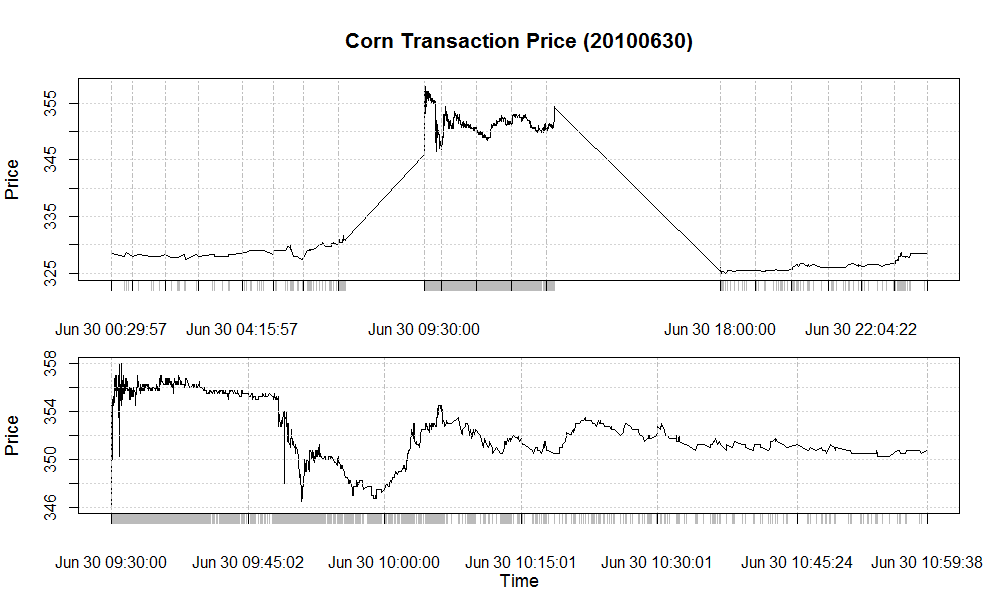
\includegraphics{images/100630.png}
\caption{Figure 2: Price of July 2010 corn on June 30, 2010 before and
after the release of Planted Acres Report.}
\end{figure}

In the top panel of Figure 2 you can see that the time stamps indicate
those are transactions occurring in the overnight electronic market.
There is a break in the morning prior to 9:30 CST when trading begins in
the daytime session. It is in this period that the Planted Acres report
is released. The bottom panel only displays the daytime session, so that
you can see the trading action more clearly. Between 9:30am and about
10:15 the market trades in a 10 cent range.

The Oct 8th WASDE report caused the market to open limit up. The
exchange sets the maximum fluctuation a futures price can trade in a
given day. The value of the limit can change at the discretion of the
exchange with some advance notice. The report indicated a sharp drop in
forecasted yield for corn. This resulted in the ending stocks number for
the 2010/2011 marketing year forecast below 1 billion bushels with a
very low stocks to use ratio as well. The market reaction is show below
in Figure 3.

\begin{figure}[htbp]
\centering
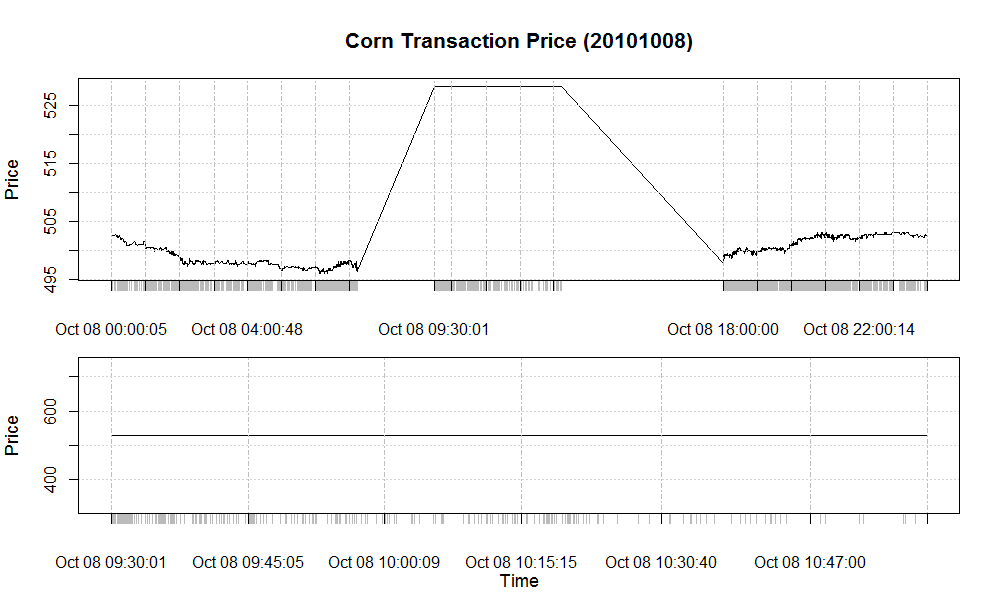
\includegraphics{images/101008.png}
\caption{Figure 3: Price of December 2010 corn on October 8th, 2010
before and after the release of the WASDE Report.}
\end{figure}

The flat line during the daytime trading session is apparent, resulting
from prices being locked at the limit during the entire trading day.

The next example is December 9th, 2010, the release day of the December
WASDE report.

\begin{figure}[htbp]
\centering
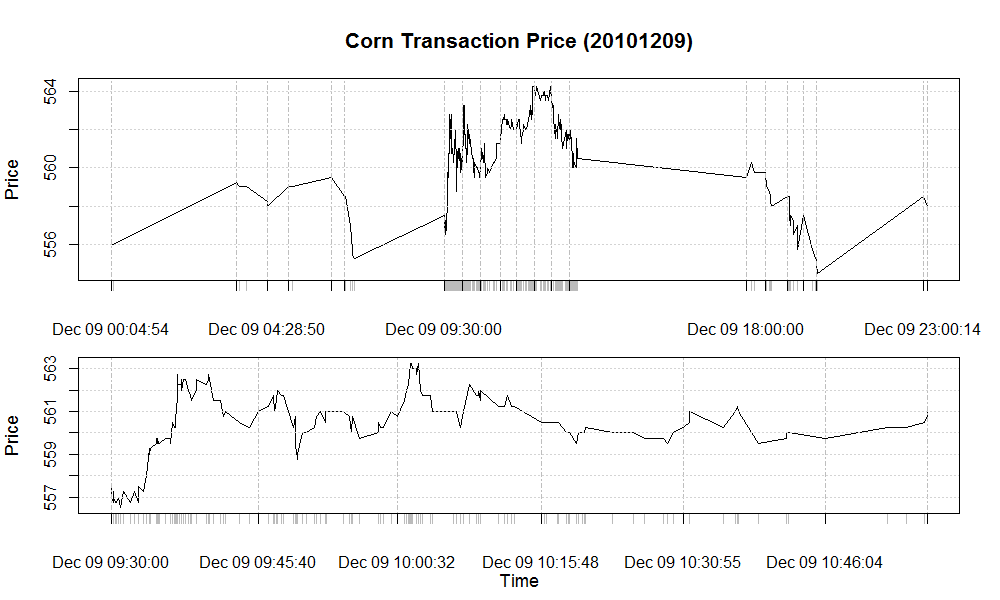
\includegraphics{images/101209.png}
\caption{Figure 4: Price of March 2011 corn on December 9th, 2010 before
and after the release of the WASDE Report.}
\end{figure}

On this day the market opened 10 cents higher, or 1.8\%. On a non-report
day, this would be a large price move. However, for a report day, it
seems like a small price adjustment.

Figure 5, below, is the price action on the March 31st, 2011, the day
the Prospective Plantings and Grain Stocks reports were released.

\begin{figure}[htbp]
\centering
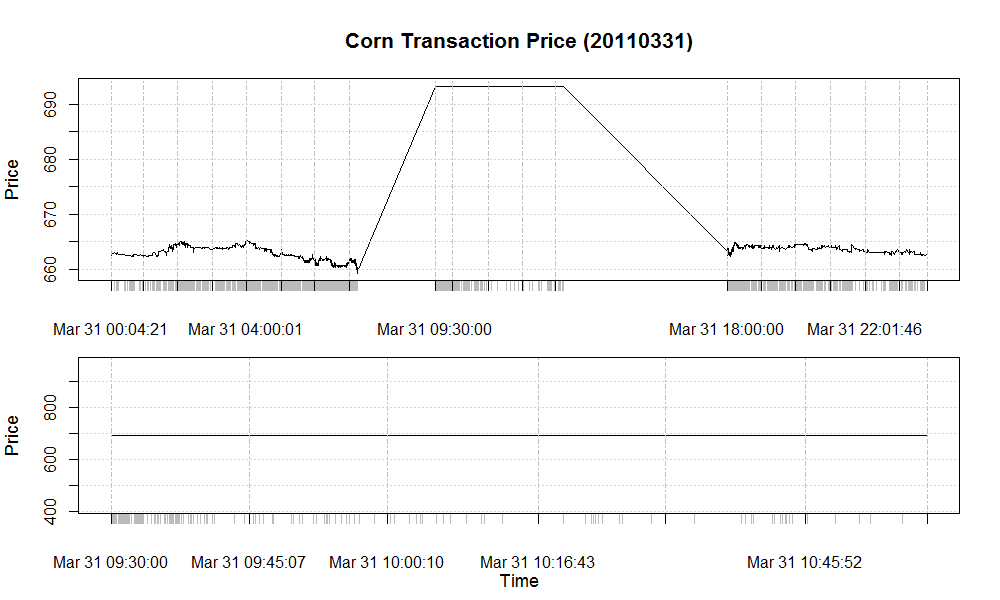
\includegraphics{images/110331.png}
\caption{Figure 5: Price of May 2011 corn on March 31st, 2011 before and
after the release of the Planted Acres Report.}
\end{figure}

This report indicated that corn acreage was to be higher than previously
expected, but corn stocks were lower than expected. The stocks number
dominated the price direction strongly and the market traded limit up on
this day as well.

\section{Conclusions}\label{conclusions}

This chapter reviewed the history of report released by the USDA. We
noted a data leak in 1905 led the agency to consider security from an
early date - a important component of report production that persists to
this day. We also learned that the Prospective Plantings, Planted
Acreage, October WASDE, January WASDE, and Grain Stocks reports are the
most likely to produce rapid price adjustments in the market. Some
specific examples were given, and depicted through charts of transaction
prices.

\chapter{Forecasting Production}\label{forecasting-production}

The preceding chapters have served as a background about agricultural
markets, and important informational events that drive commodity prices.
Going forward, we will focus our energy on the more data and technical
questions of actually forecasting elements of the balance sheet - and
later, short term price changes using time-series econometric
techniques. In the remainder of this chapter, the discussion and figures
are all for corn.

Our first task in forecasting a balance sheet will be to get a good
estimate of production for the marketing year. As we noted before,
\texttt{Production\ =\ Acreage\ X\ Yield}. To begin, we will discuss the
fundamentals of estimating acreage.

\section{Estimating Acreage}\label{estimating-acreage}

Like many other agricultural variables we would like to forecast, our
methodology for forecasting acreage depends on the time of year we are
making the forecast. Prior to planting season, we can rely on recent
trends in acreage from previous years, plus relative profitability of
planting competing crops as measured by relative futures prices.

Historical acres planted and harvested can be found from USDA NASS.

\begin{quote}
\section{Steps to download historical acreage
data:}\label{steps-to-download-historical-acreage-data}

\begin{enumerate}
\def\labelenumi{\arabic{enumi}.}
\tightlist
\item
  Go to \url{https://www.nass.usda.gov/Quick_Stats/Lite/index.php}
\item
  Click \emph{Crops} in the menu
\item
  In the query, choose \emph{Field Crops}
\item
  Choose corn
\item
  Click \emph{Acreage, Yeild, Production, and Price}
\item
  Select the years you want. Hold the Ctrl key to select multiple.
\item
  Click \emph{Get Data}.
\end{enumerate}
\end{quote}

\begin{figure}[htbp]
\centering
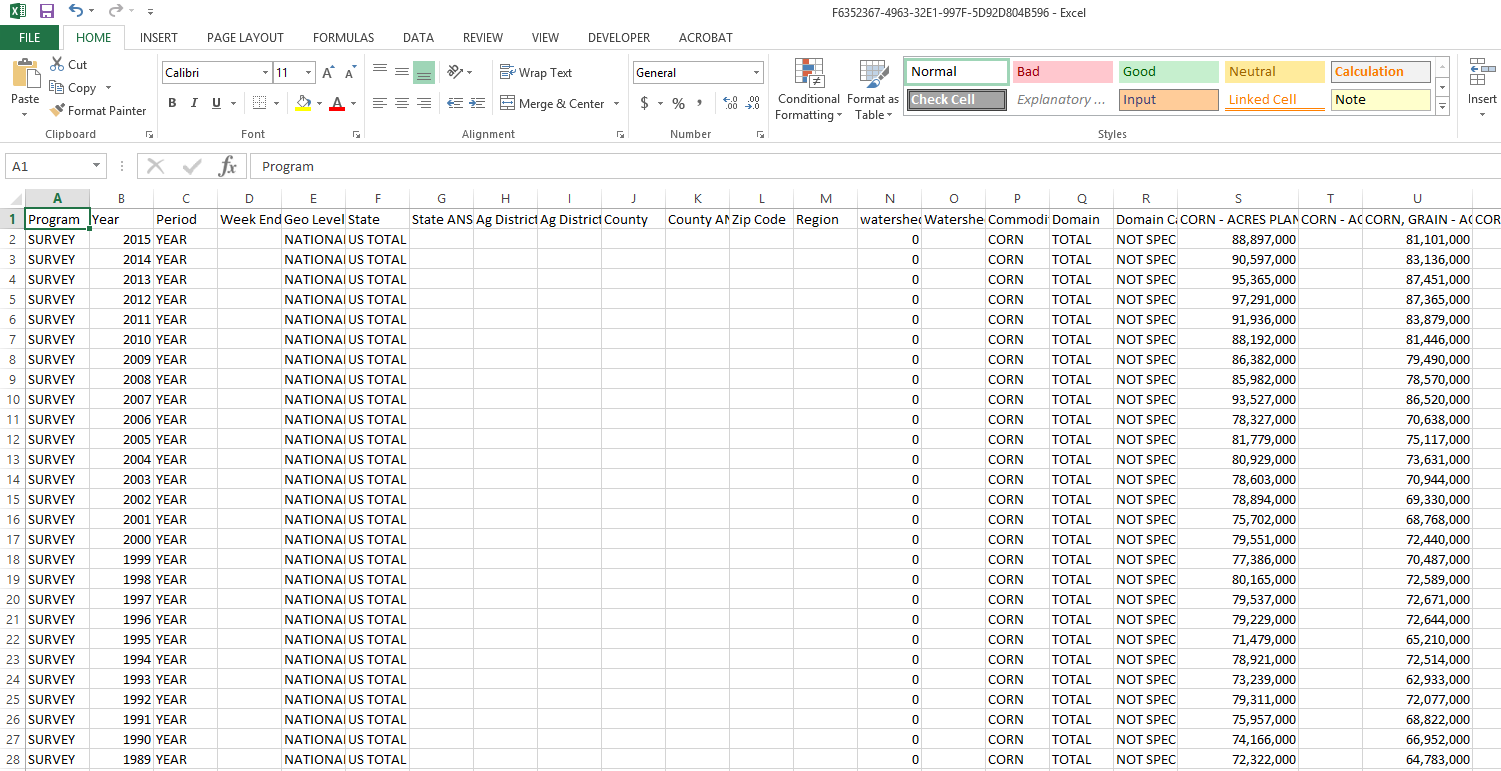
\includegraphics{images/ACRES_historical.png}
\caption{Figure 1: Historical Acreage Data}
\end{figure}

The following is a graph of historical corn \emph{Planted Acres} along
with the ratio of \emph{Average Prices Received by Farmers} for corn and
soybeans.

\begin{figure}[htbp]
\centering
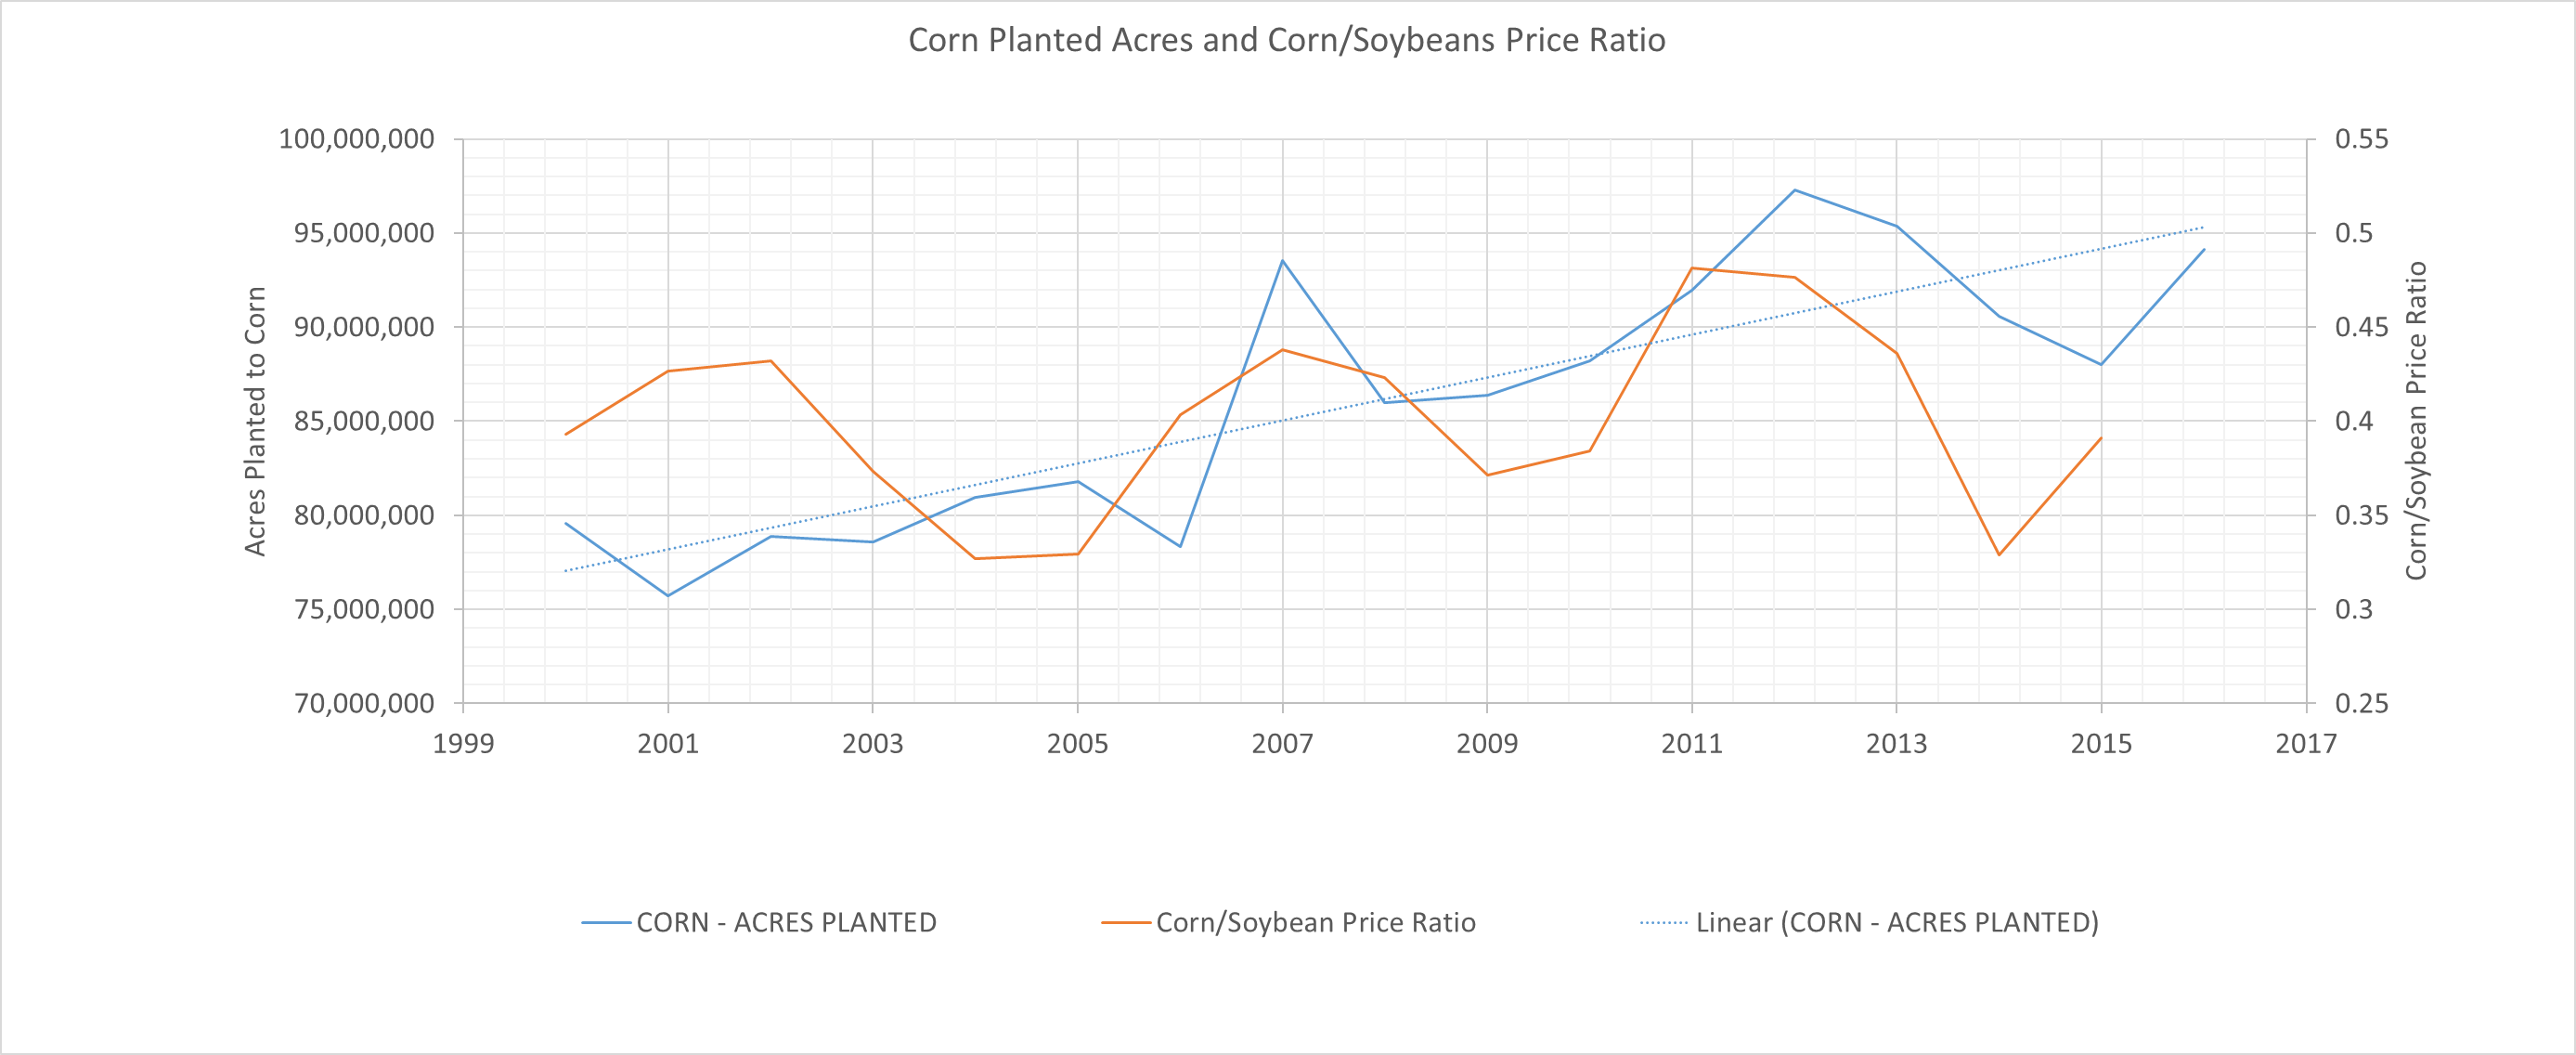
\includegraphics{Excel-files/ForecastingProduction-HistoricalAcreage_files/image003.png}
\caption{Figure 2: Corn Planted Acres and Corn/Soybean Price Ratio}
\end{figure}

The following is a graph of historical corn \emph{Planted Acres and
Harvested Acres} generated from the data described above from 2000 to
2014. The left axis shows planted and harvested acres while the right
axis shows the difference between the two. Since 2000, you can see that
corn acreage has been increasing steadily from 80 million acres to just
above 90 million acres. Given this, prior to planting season we might
expect a simple trend-line to forecast corn acreage fairly well.
However, notice that in a couple of instances there were fairly large
deviations from the trend-line.

\begin{figure}[htbp]
\centering
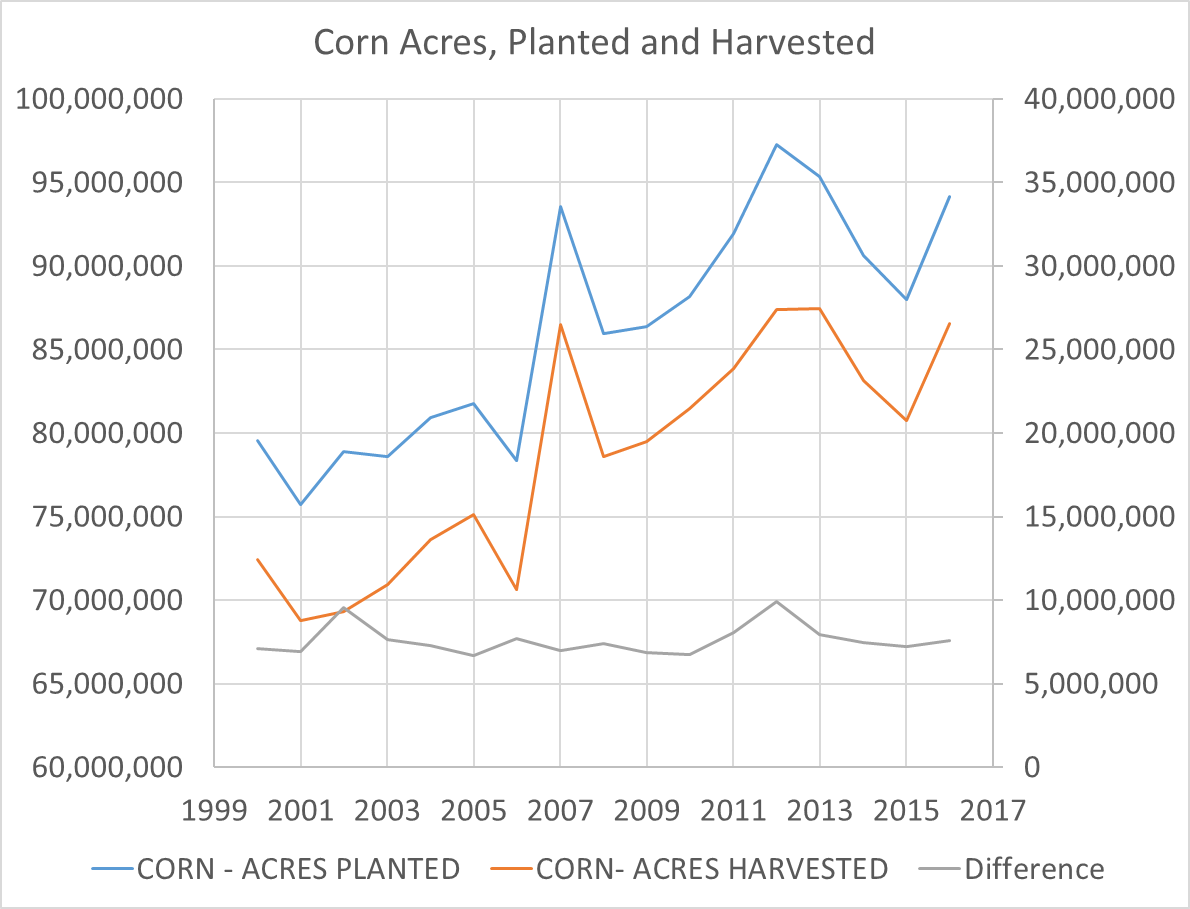
\includegraphics{Excel-files/ForecastingProduction-HistoricalAcreage_files/image001.png}
\caption{Figure 3: Corn Planted Acres and Harvested Acres, 2000-2014}
\end{figure}

Aside from historical trends, if one considers the decision the average
corn farmer makes, he or she considers the relative profitability of
planting corn versus planting soybeans. In years where profitability
favors corn, more corn-on-corn acres will be planted, thus increasing
the total number of acres planted to corn. In years where profitability
favors soybeans, less corn-on-corn acres will be planted, thus
increasing soybean acres and reducing the total number of acres planted
to soybeans. This pattern is demonstrated in 2008 and 2011 when an
increase in the corn-to-soybean price ratio corresponded to an increase
in planted acres.

Based on the information in Figure 2, one might predict a decline in
corn planted acres in the spring of 2015. Although, at the time of
planting, the November soybean and December corn futures prices will be
the appropriate prices to use for this analysis, because they represent
expected profit.

For example, the following graph shows the December 2016 and November
2016 corn and soybean futures prices respectively for 8/1/2015 to
9/10/2015. The ratio is not graphed here, but since the price of corn is
rising relative to the price of soybeans, the relative profitability has
drifted toward corn over this time frame. Assuming inputs costs were
constant, forecasts of corn and soybean acreage for Spring 2016 would
take this into account.

\begin{figure}[htbp]
\centering
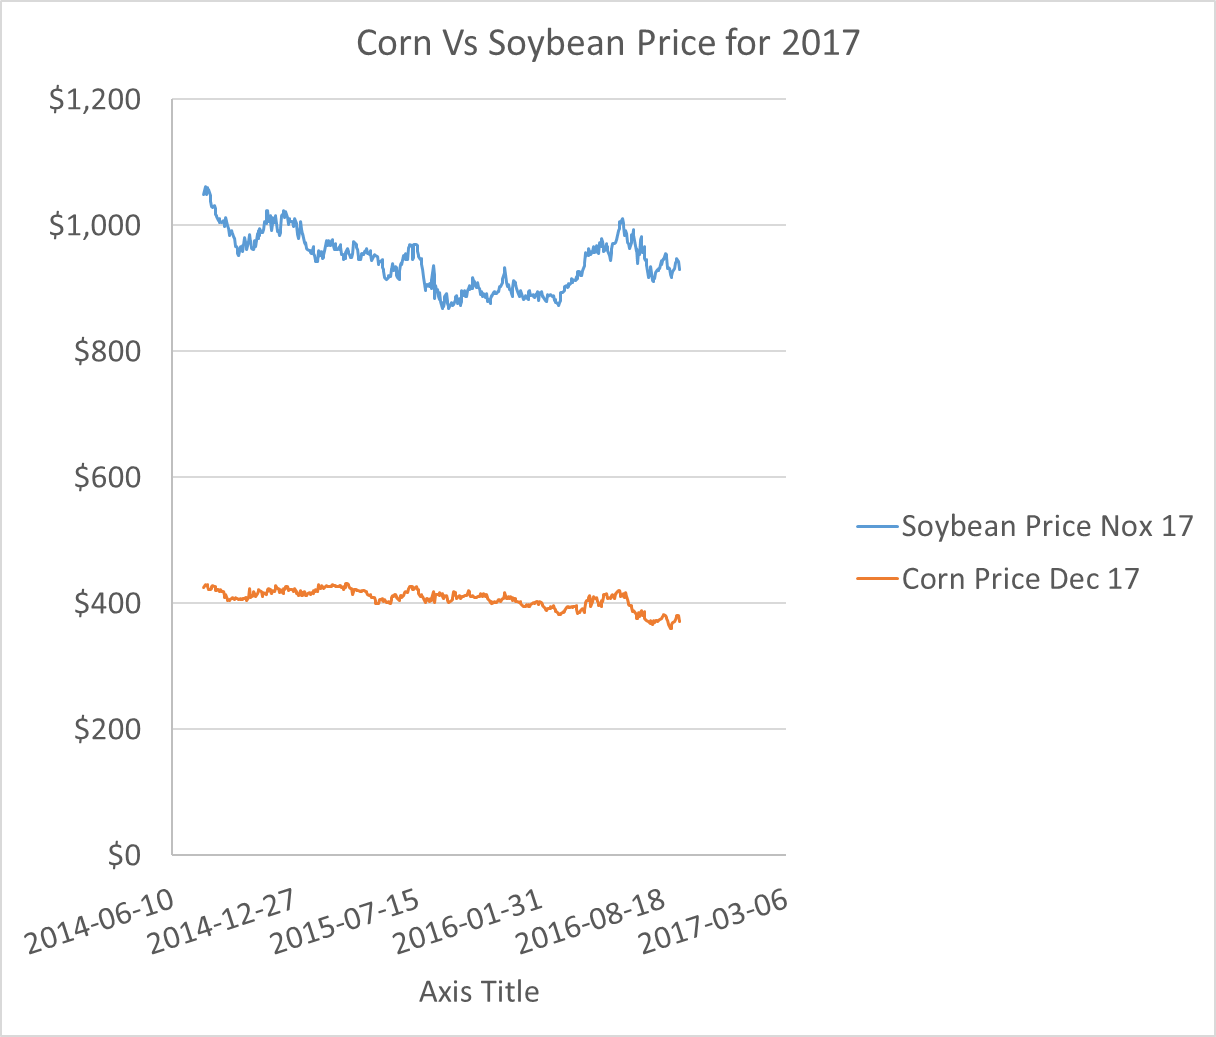
\includegraphics{images/c-s2017.png}
\caption{Figure 4: 2016 Corn (December) and Soybean (November) Futures
Prices from 8/1/2016 to 9/15/2016}
\end{figure}

\subsection{Forecasting Harvested
Acres}\label{forecasting-harvested-acres}

After forecasting \emph{Planted Acres} one still needs to provide a
forecast for \emph{Harvested Acres}. Figure 3 shows historical trends in
\emph{Harvested Acres} relative to \emph{Planted Acres}. The difference
between these two variables is provided in grey with units along the
right axis for convenience.

Harvested acres tends to be a fairly stable number, averaging 7.6
million acres between 2000 and 2014. Although, years when this variable
deviates most from trend corresponds to years of exceptionally poor
production. See 2012 and 2002 as examples. These years marginal
reductions in production are explained by reduced yield and abandoned
acres, so forecasting the harvested acres number accurately becomes very
important to accurately forecasting production in shortfall years.

\section{Forecasting Yield}\label{forecasting-yield}

Just like in forecasting acreage, we have different procedures for
forecasting yield prior to planting. Before the summer growing season
gets underway trend yield is usually used. The trouble is, where to
start?

\begin{figure}[htbp]
\centering
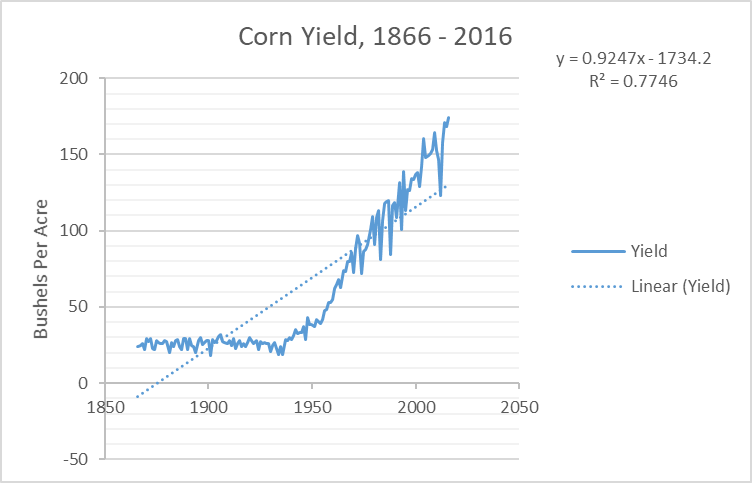
\includegraphics{Excel-files/ForecastingProduction-HistoricalAcreage_files/image005.png}
\caption{Figure 5: Historical Yields since 1866}
\end{figure}

USDA has records on yield that go back to 1866. While one often thinks
more information is better when forecasting, the old yield estimates are
no longer useful for forecasting current yield. Technological progress
caused yields to take of in the 1950's and they have been climbing ever
since. In the forecasting world, this is called \emph{structural change}
or a \emph{structural break}. If \emph{structural change} has occurred,
the world looks so different now than it did before the structural
change that data from before the break just is not useful for
forecasting going forward.

It turns out that if you estimate a trend-line beginning with 1952, with
1980, or with pretty much any date in between, you will get an estimate
that is roughly similar.

\begin{figure}[htbp]
\centering
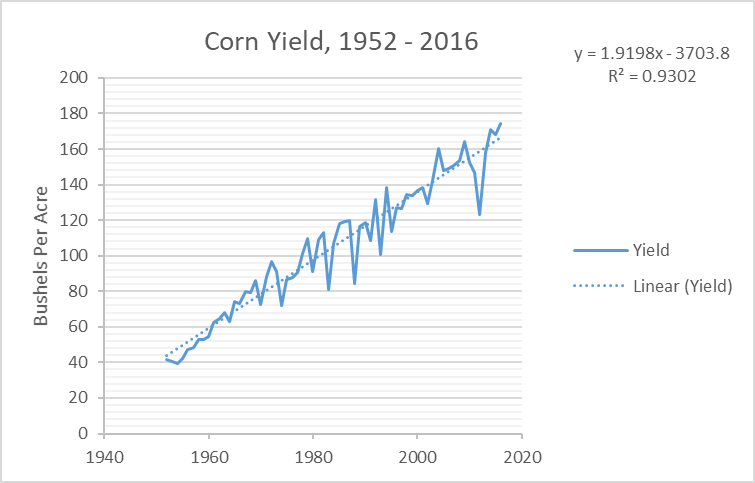
\includegraphics{Excel-files/ForecastingProduction-HistoricalAcreage_files/image007.png}
\caption{}
\end{figure}

\begin{figure}[htbp]
\centering
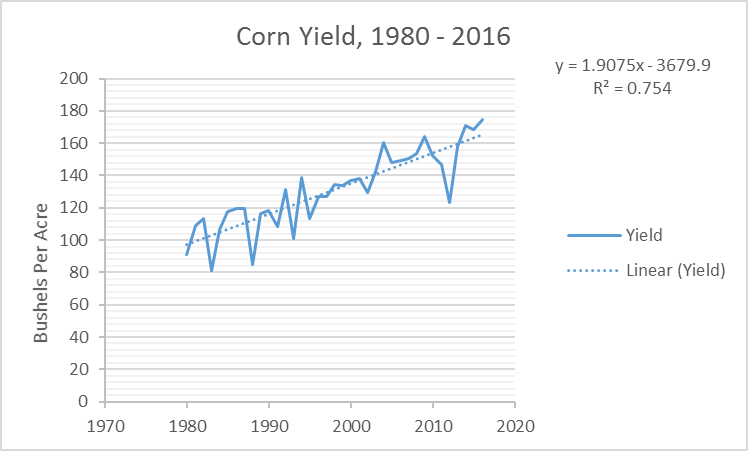
\includegraphics{Excel-files/ForecastingProduction-HistoricalAcreage_files/image013.png}
\caption{Figure 6: Historical Yields since 1952 and 1980}
\end{figure}

For example, using the trend-line beginning with 1952 to forecast yield
we come up with \(Yield^{2015} = 1.9066*2015 - 3677.9 = 163.899\).
While, using the trend-line beginning with 1980 to forecast yield we
come up with \(Yield^{2015} = 1.8619*2015 - 3588.9 = 162.8285\).In other
words, yields have been increasing by an average of just under 2 bushels
per acre since the 1950's.

\section{Growing Season Yield
Forecasts}\label{growing-season-yield-forecasts}

The USDA undertakes an extensive effort to estimate yield during the
growing season. Prior to August, they conduct the \textbf{Agricultural
Yield Survey} (AYS) which surveys a large number of farmers and asks
them to estimate yield. Beginning in August, the USDA conducts what it
calls the \textbf{Objective Yield Survey}. They take samples from a
relatively large number of fields and estimates yield in those fields
based on various factors such as counts of plants, ears, and pods (for
soybeans) \citep{good2011yield}.

Since commodity futures markets respond to new information in the USDA
reports, analysts employed by private advisory firms or proprietary
trading shops will try to anticipate the USDA's yield forecast. If they
can do this they can capitalize on superior private information by
making a well advised business decision or earning speculative profits.

This is difficult because an independent analyst will not have the same
level of resources as the USDA does when it compiles its monthly yield
estimates; he or she will have to rely on historical data and an
understanding of how weather is affecting crop yields across the
geographically dispersed growing region. Figure 8 below plots each
year's deviation from trend yield since 1980. The first plot is in
levels (i.e., \(Yield_t - Trend Yield_t\)); whereas the second plot is
in percent terms (i.e., \(\ln{Yield_t} - \ln{Trend Yield_t}\). Notice
that the shape looks roughly the same, but the 2012 drought looks worse
expressed in level deviations than the short crops of 1983, 1988, and
1993. This is because yield is trending higher. In percentage terms we
see that the 2012 drought was equally as bad as 1983 and not quite as
bad as 1988.

\begin{figure}[htbp]
\centering
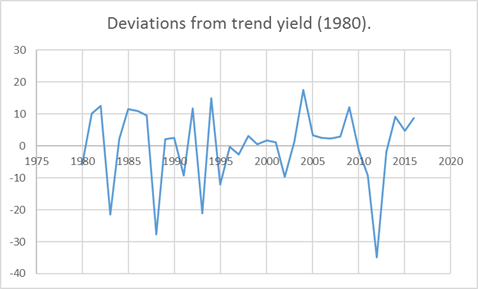
\includegraphics{Excel-files/ForecastingProduction-HistoricalAcreage_files/image016.png}
\caption{}
\end{figure}

\begin{figure}[htbp]
\centering
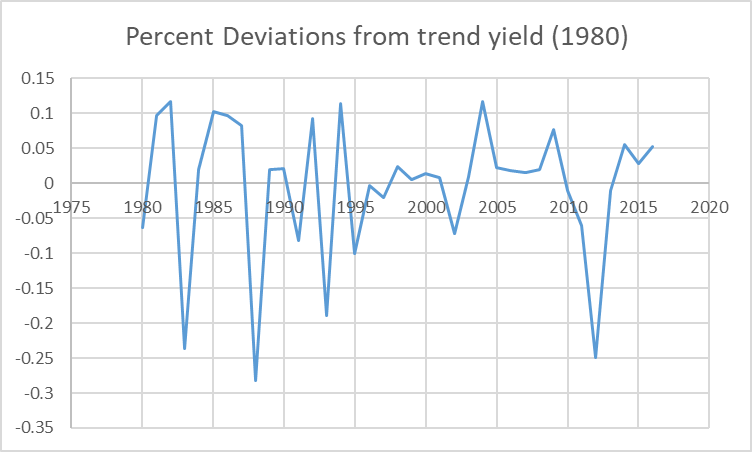
\includegraphics{Excel-files/ForecastingProduction-HistoricalAcreage_files/image017.png}
\caption{Figure 7: Deviations from Trend in both Level and Percent
(using trend since 1980)}
\end{figure}

Short of an advanced agronomic model that can take into account planting
date, precipitation,
\href{https://en.wikipedia.org/wiki/Growing_degree-day}{growing degree
days}, or ability to estimate yield from remote sensing technology
\citep{unganai1998drought}, we will have to resort to the \emph{similar
year approach}.

Analysts often estimate deviations from trend yield by finding year
similar to the current one in terms of weather. The assumption is that
if the weather patterns were similar then the percent deviation from
trend yield should be similar as well. Note here that percent deviation
is preferable so you do not need to adjust for the increasing trend in
yield as you look backward to a similar year.

An alternative approach would be to use the \emph{Crop Condition Report}
and find a year in recent history that had a similar percent of the crop
rated \emph{Good/Excellent}. Figure 8 below shows how \emph{Good} +
\emph{Excellent} crop condition ratings relate to percent deviations in
trend yield. They should be at least positively correlated, and in fact
starting in the late 90's this measure began to correlate strongly with
the final yield.

\begin{figure}[htbp]
\centering
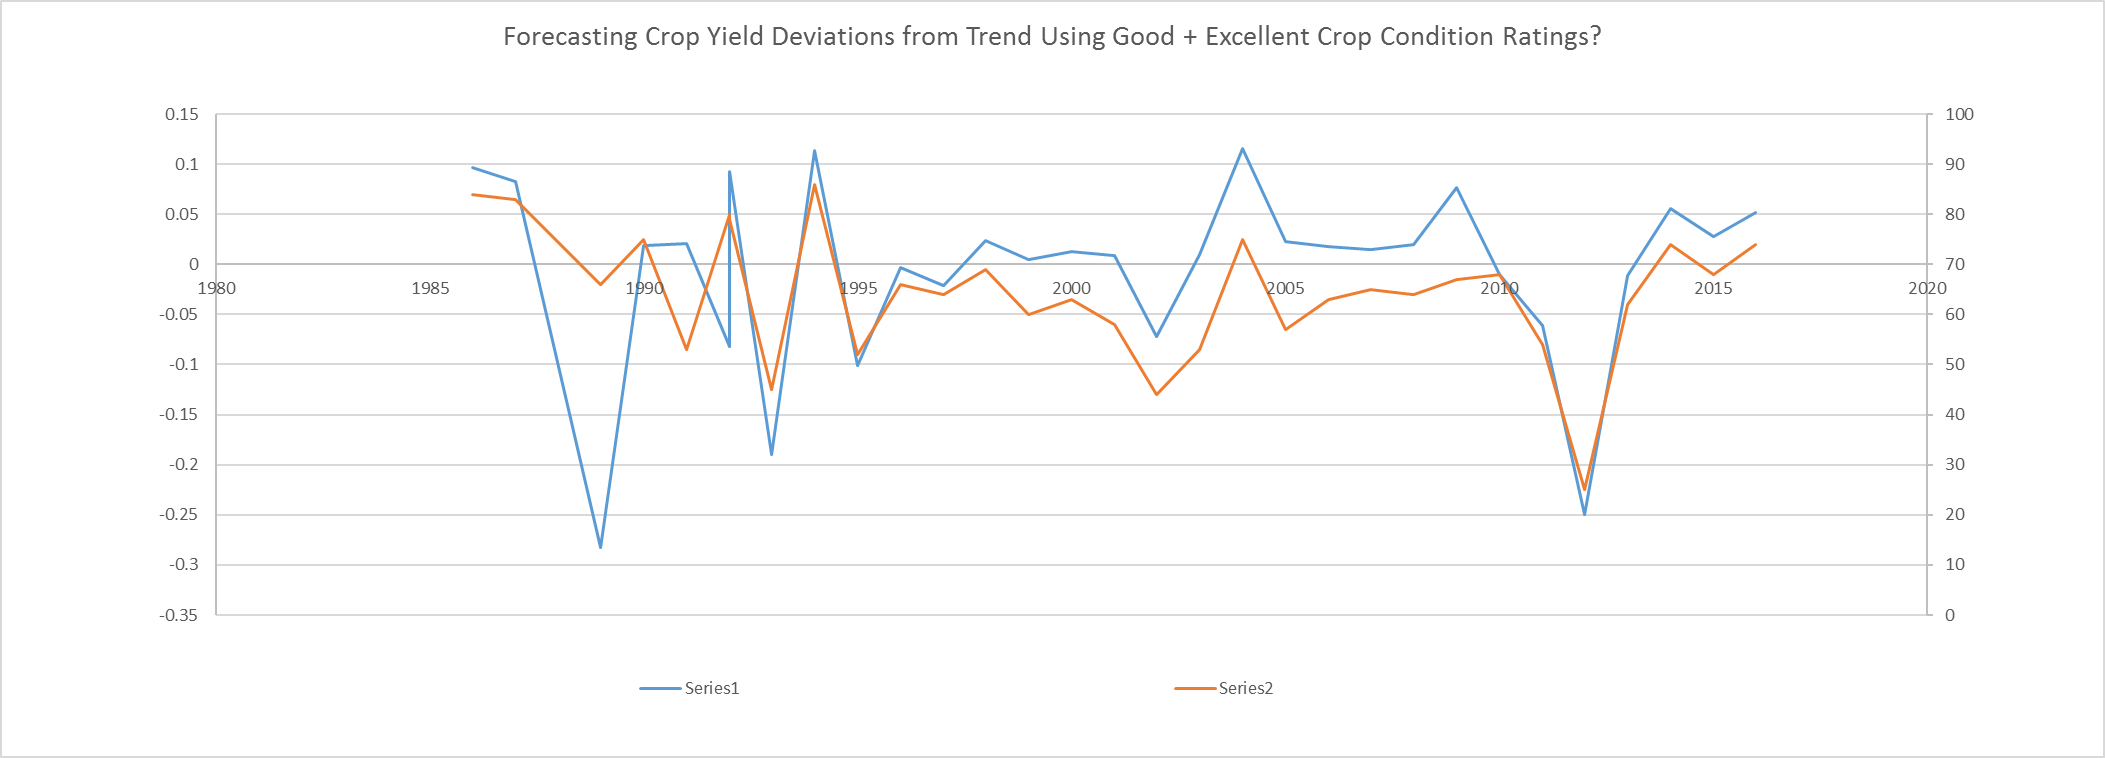
\includegraphics{Excel-files/ForecastingProduction-HistoricalAcreage_files/image021.png}
\caption{Figure 8: \emph{Good} plus \emph{Excellent} Crop Condition
Ratings in Final Week of Reporting versus Percent Deviations in Yields}
\end{figure}

\section{Forecasting Production}\label{forecasting-production-1}

Once you have an estimate for acreage and yield, you can multiply them
to give you an estimate of production for your balance sheet forecast.

\section{Conclusion}\label{conclusion-1}

In this chapter we discussed the basics of forecasting production. First
we discussed forecasting acreage, then we moved on to forecasting yield
both before and during the growing season. We discovered that estimating
yield percent deviations from trend better than the USDA is extremely
difficult. Even anticipating whether the yield forecast will go up or
down is not an easy task. The \emph{similar year method} has its
limitations when used to find similar years in terms of weather or crop
conditions ratings.

\section{Exercises}\label{exercises-3}

\begin{enumerate}
\def\labelenumi{\arabic{enumi}.}
\item
  Use NASS data for soybeans for forecast production in a similar manner
  we we did in class for corn.
\item
  Read and Discuss:
  \href{http://farmdocdaily.illinois.edu/2015/05/early-planting-and-2015-corn-yield-prospects.html}{Early
  Planting and 2015 Corn Yield Prospects: How Much of an Increase?}

  \begin{itemize}
  \tightlist
  \item
    Irwin, S., D. Good, and J. Newton. ``Early Planting and 2015 Corn
    Yield Prospects: How Much of an Increase?'' farmdoc daily (5):93,
    Department of Agricultural and Consumer Economics, University of
    Illinois at Urbana-Champaign, May 20, 2015.
  \end{itemize}
\end{enumerate}

\chapter{Forecasting Use of Corn}\label{forecasting-use-of-corn}

In the WASDE balance sheet for corn there are three use categories. Two
account for domestic consumption - Food, Seed and Industrial, and Feed
and Residual - while exports make up the third category. Ethanol makes
up a large portion of the Food, Seed, and Industrial category, so it is
given its own line in the balance sheet.

As we have noted before, historical use patterns are the first place to
start when trying to forecast use categories for the marketing year.
Looking at quarterly gives you a sense of how use is distributed across
the marketing year in different categories. The annual histories,
however, are probably the most useful.

\section{Food, Alcohol, and Industrial
Use}\label{food-alcohol-and-industrial-use}

Let us begin by looking at the Food, Alcohol and Industrial category.
These data were queried from the
\href{http://www.ers.usda.gov/data-products/feed-grains-database/feed-grains-yearbook-tables.aspx\#26780}{Feed
Grains database} maintained by the USDA ERS. The categories here are a
little more disaggregated than those presented in the USDA WASDE balance
sheets, but they are roughly the same. For example, in figure 1 below we
show the \emph{Food, Alcohol, and Industrial} use category. This omits
seed from the \emph{Food, Seed, and Industrial} category in the WASDE
balance sheet. The Feed Grains database actually breaks out the seed use
as its own column, but corn used for seed is a very small proportion of
production and it is largely predictable from year to year.

\begin{figure}[htbp]
\centering
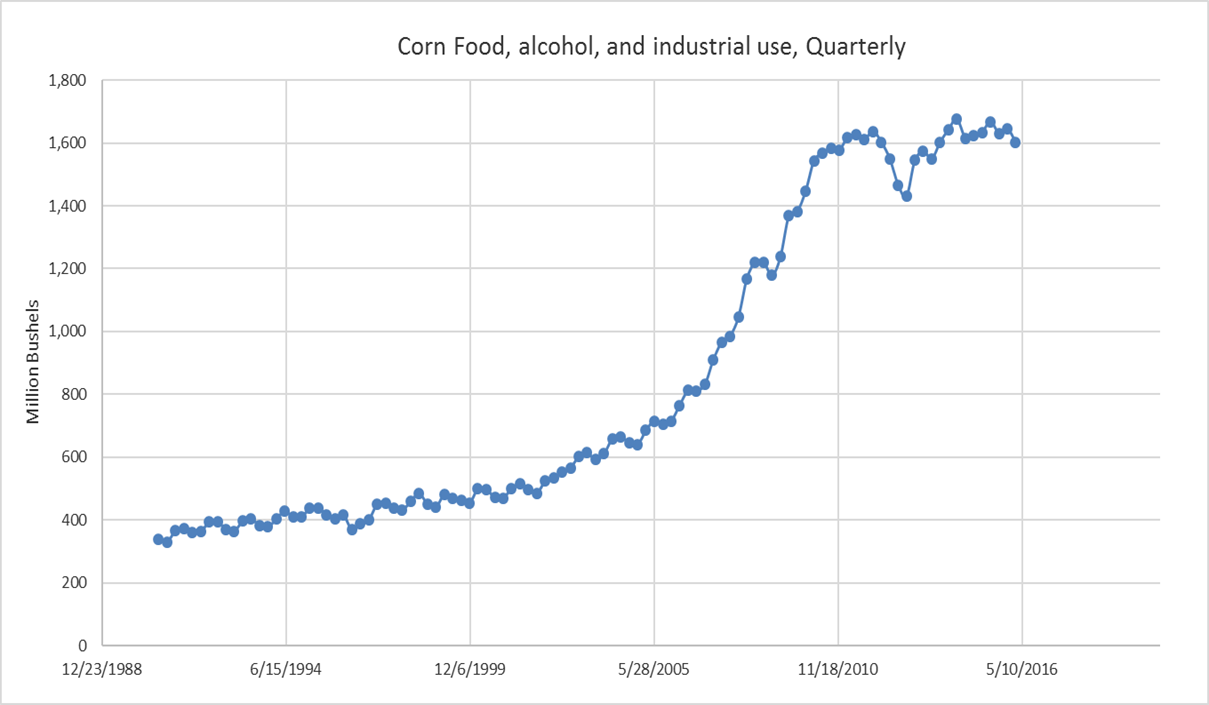
\includegraphics{Excel-files/IntroductiontoCommodityTS-FeedGrains_Corn_files/image013.png}
\caption{Figure 1: Corn Food, Alcohol, and Industrial Use, Quarterly
1990-2015}
\end{figure}

Source:
\href{http://www.ers.usda.gov/data-products/feed-grains-database/feed-grains-yearbook-tables.aspx\#26780}{Feed
Grains database} maintained by the USDA ERS.

Figure 1 shows a dramatic uptrend in the Food, Alcohol and Industrial
use category. This is due to the dramatic increase in the production of
ethanol starting around 2005/2006 and plateauing around 2010 when U.S.
ethanol consumption roughly hit the `blend-wall' where ethanol makes up
10\% of the retail gasoline supply.

\begin{figure}[htbp]
\centering
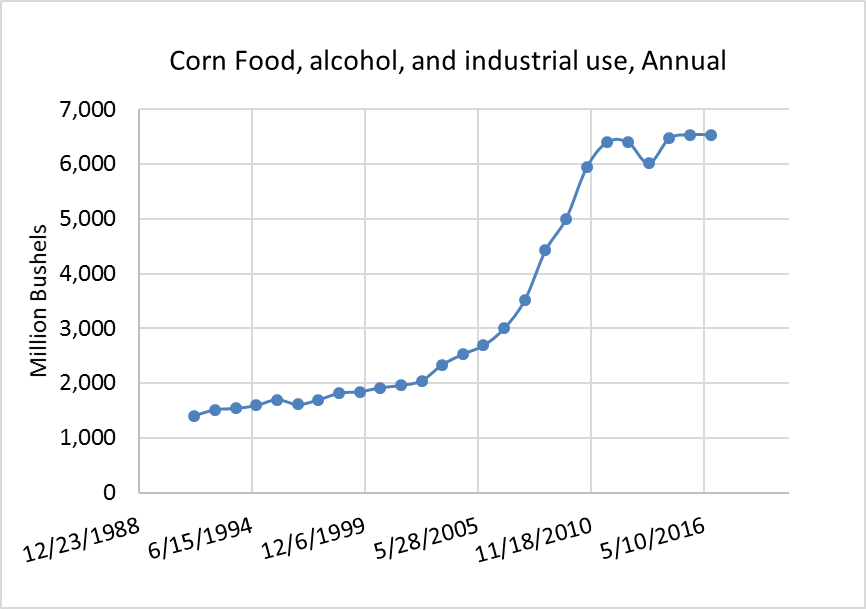
\includegraphics{Excel-files/IntroductiontoCommodityTS-FeedGrains_Corn_files/image001.png}
\caption{Figure 2: Corn Food, Alchohol, and Industrial Use, Annual
1990-2015}
\end{figure}

Source:
\href{http://www.ers.usda.gov/data-products/feed-grains-database/feed-grains-yearbook-tables.aspx\#26780}{Feed
Grains database} maintained by the USDA ERS.

Figure 2 shows the same data, but the quarterly figures are aggregated
to the marketing year total. In both figures 1 and 2 the rationing
effects of high prices that occurred as a result of the drought in 2012.

\begin{figure}[htbp]
\centering
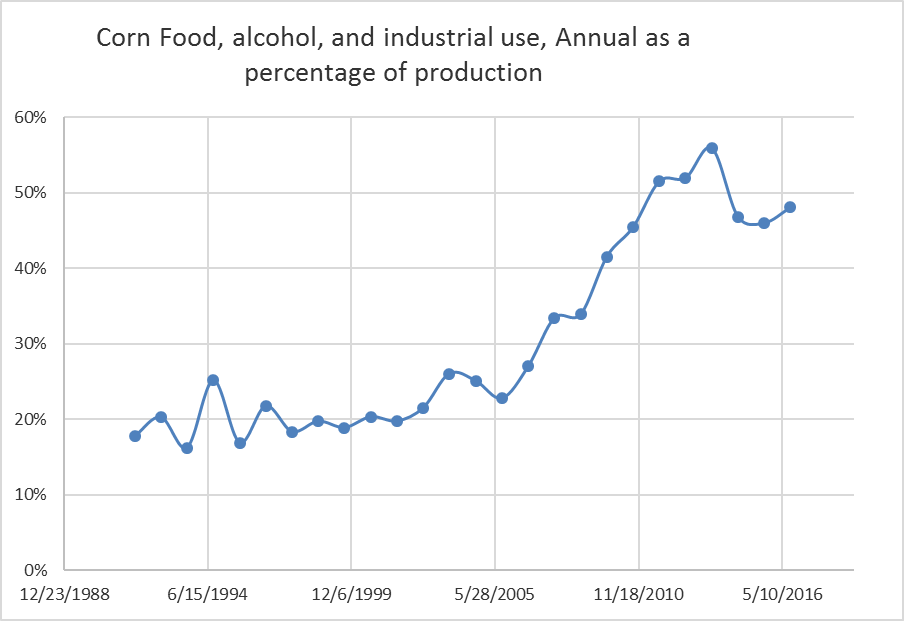
\includegraphics{Excel-files/IntroductiontoCommodityTS-FeedGrains_Corn_files/image009.png}
\caption{Figure 3: Corn Food, Alchohol, and Industrial Use, Annual
1990-2016 as a percentage of production}
\end{figure}

Source:
\href{http://www.ers.usda.gov/data-products/feed-grains-database/feed-grains-yearbook-tables.aspx\#26780}{Feed
Grains database} maintained by the USDA ERS.

From figure 3 it is easier to see what share of the crop the large
increase in corn use in the Food, Alcohol, and Industrial use category.
In figure 3 this use category is presented as a percentage of that
marketing year's production. In the early 1990's this use category
accounted for over 50\% since 2010. The drop in percentage of production
in 2015 occurs because of the large crop in 2015, even though the use
level is flat (shown in figure 2).

\section{Exports}\label{exports}

Quarterly corn exports are displayed in figure 4. Unlike Food, alcohol
and industrial use, exports tend to have a very seasonal or cyclical
pattern. Exports are large in the second quarter of the marketing year,
December to February, right after we harvest the new crop. This is when
stocks are most plentiful and prices are at season lows in years
exhibiting an upward sloped forward curve.

\begin{figure}[htbp]
\centering
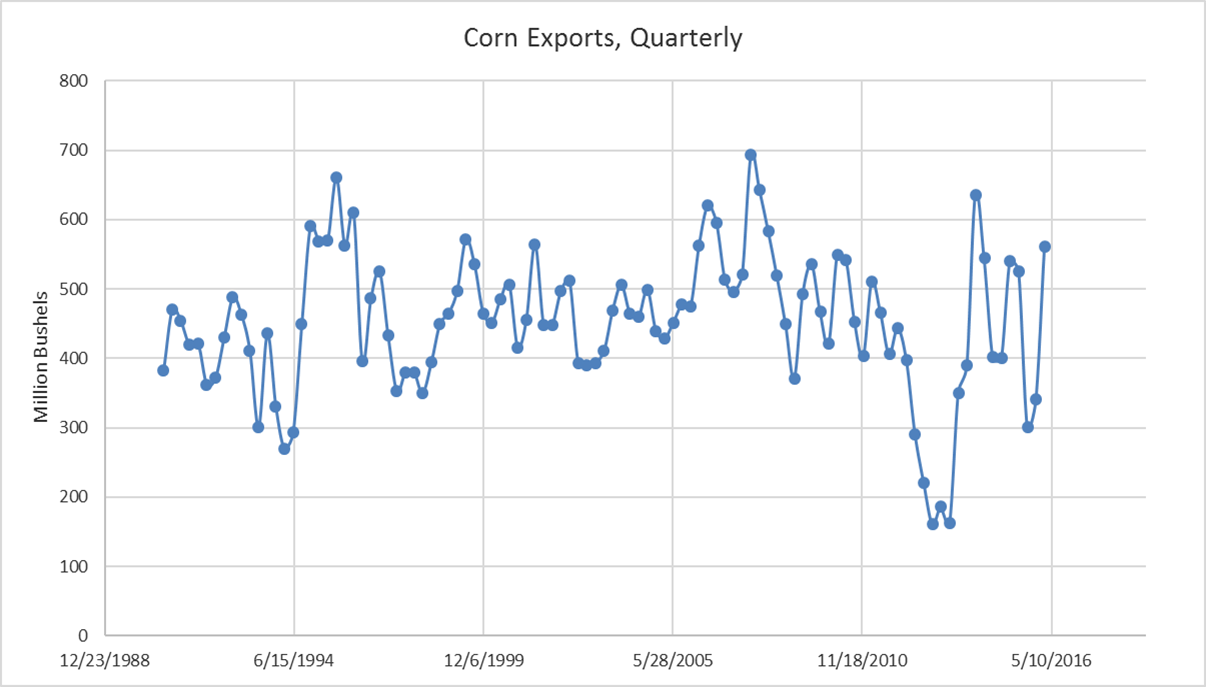
\includegraphics{Excel-files/IntroductiontoCommodityTS-FeedGrains_Corn_files/image014.png}
\caption{Figure 4: Corn Exports, Quarterly 1990-2015}
\end{figure}

Source:
\href{http://www.ers.usda.gov/data-products/feed-grains-database/feed-grains-yearbook-tables.aspx\#26780}{Feed
Grains database} maintained by the USDA ERS.

Displaying the same data in Figure 5, but aggregating to an annual
frequency, we see the marketing seasonality smoothed away.

\begin{figure}[htbp]
\centering
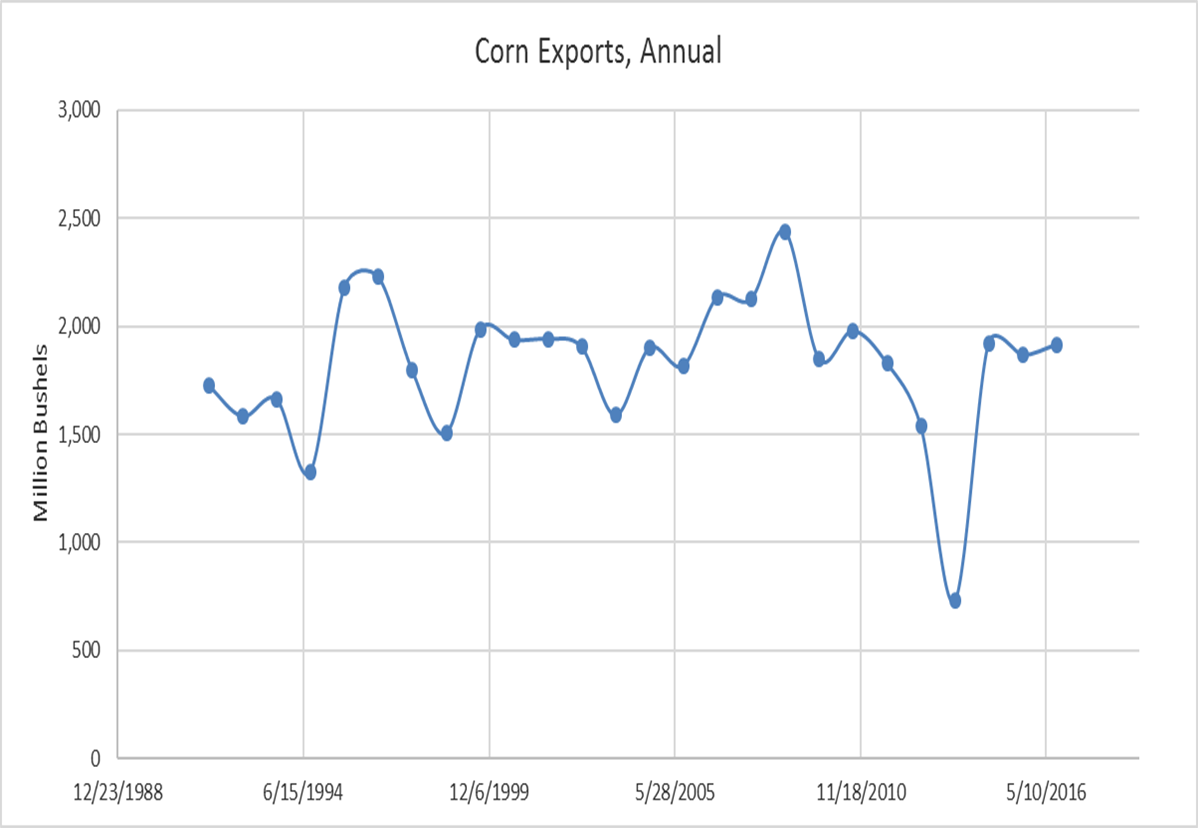
\includegraphics{Excel-files/IntroductiontoCommodityTS-FeedGrains_Corn_files/image023.png}
\caption{Figure 5: Corn Exports, Annual 1990-2015}
\end{figure}

Source:
\href{http://www.ers.usda.gov/data-products/feed-grains-database/feed-grains-yearbook-tables.aspx\#26780}{Feed
Grains database} maintained by the USDA ERS.

On average, it appears that exports follow a constant trend-line with
variation around the mean produced by years of surplus or scarcity. The
drought year 2012, for example is clearly visible as an exceedingly low
export year.

In figure 6 we display annual corn exports as a percentage of corn
production.

\begin{figure}[htbp]
\centering
\includegraphics{Excel-files/IntroductiontoCommodityTS-FeedGrains_Corn_files/image029.png}
\caption{Figure 6: Corn Exports, Annual 1990-2016 as a percentage of
corn production}
\end{figure}

Source:
\href{http://www.ers.usda.gov/data-products/feed-grains-database/feed-grains-yearbook-tables.aspx\#26780}{Feed
Grains database} maintained by the USDA ERS.

When exports are viewed as a proportion of production, we see a
pronounced downward trend. This is due to the increasing share of
production allocated to the Food, seed, and Industrial category visible
in figure 3. Recall that this category is comprised mainly of corn as
feed-stock for ethanol production.

The year-to-year variation is caused by price fluctuations with low
prices encouraging and high prices discouraging consumption.

: Table 1: Top 10 Importers of U.S. Corn 2011/2012 through 2015/2016
Marketing Years, Ranked in Descending Order for Marketing Year 20152016
(1,000 Metric Tons)

\begin{tabular}{l|l|l|l|l|l|l|l|l|l|l}
\hline
COUNTRY & EXPORTS 2015/2016 & RANK & EXPORTS 2014/2015 & RANK & EXPORTS 2013/2014 & RANK & EXPORTS 2012/2013 & RANK & EXPORTS 2010/2011 & RANK\\
\hline
MEXICO & 12558.6 & 1 & 10793.8 & 2 & 10526.3 & 2 & 4370.0 & 2 & 9537.5 & 2\\
\hline
JAPAN & 10506.6 & 2 & 11858.6 & 1 & 11487.0 & 1 & 7000.2 & 1 & 11748.6 & 1\\
\hline
COLOMB & 4629.5 & 3 & 4413.3 & 3 & 3359.4 & 4 & 94.9 & 17 & 275.1 & 16\\
\hline
KOR REP & 3021.6 & 4 & 3927.2 & 4 & 4844.2 & 3 & 416.2 & 6 & 3635.3 & 4\\
\hline
PERU & 2490.9 & 5 & 2421.0 & 5 & 1414.5 & 8 & 0.0 & 0 & 0.0 & 0\\
\hline
TAIWAN & 2045.2 & 6 & 1755.0 & 6 & 1936.4 & 7 & 511.8 & 5 & 1265.4 & 6\\
\hline
S ARAB & 1516.4 & 7 & 1312.7 & 8 & 1021.0 & 9 & 344.6 & 7 & 294.8 & 15\\
\hline
EGYPT & 969.2 & 8 & 1487.0 & 7 & 2559.5 & 6 & 0.0 & 0 & 544.9 & 9\\
\hline
VENEZ & 942.3 & 9 & 701.8 & 12 & 1017.2 & 10 & 1158.1 & 4 & 1280.1 & 5\\
\hline
GUATMAL & 897.1 & 10 & 936.7 & 9 & 783.9 & 11 & 209.2 & 11 & 549.1 & 8\\
\hline
Total & 39577.4 & NA & 39607.1 & NA & 38949.4 & NA & 14105.0 & NA & 29130.8 & NA\\
\hline
\end{tabular}

Source: \href{http://apps.fas.usda.gov/export-sales/myrk_rpt.htm}{USDA
FAS} TOTAL is total exports to all countries, so summing the rows of
table 1 will not add up to the TOTAL row.

Table 1 shows the top 10 importers of U.S. corn for the 2014/2015
marketing year. Export totals are given in 1,000 metric ton units.
Clearly Japan and Mexico are the dominant Importers of U.S. corn. The
table shows that most countries rank has remained fairly stable across
the marketing years shown. Columbia is an exception to this rule. It was
ranked 17, 16, and 14 in 2012/2013, 2011/2012, and 2010/2011 marketing
years respectively, but jumped to 3rd and 4th in the 2014/2015 and
2013/2014 marketing years.

\section{Feed and Residual}\label{feed-and-residual}

The final use category is the most difficult to forecast because its
quantity is derived, not estimated. This means the USDA makes estimates
of every other row in the balance sheet. Then, to ensure the numbers add
up, they infer the Feed and Residual category by subtracting the other
demand categories from supply.

\(Feed\&Residual = Production + Imports + Beginning Stocks - Ending Stocks - FoodSeed\&Industrial - Exports\)

Since each category on the right hand side is itself estimated with some
error, the error for the Feed and Residual category is the sum of the
errors of the other categories. This means that forecast errors from
each of the categories get added together, creating a category with
larger forecast error than all the others. For this reason the Feed and
Residual category is the most difficult to forecast. It should correlate
roughly to livestock feeding units, but does not prove to be that
effective in practice.

\(\begin{align} Feed\&Residual = (Production + \epsilon_{prod}) + (Imports + \epsilon_{import}) + (Beginning Stocks + \epsilon_{BStocks}) \\ - (Ending Stocks + \epsilon_{EStocks}) - (FoodSeed\&Industrial + \epsilon_{Food}) - (Exports + \epsilon_{Export}) \end{align}\)

Figure 7 below displays the Feed and Residual category since 1990.

\begin{figure}[htbp]
\centering
\includegraphics{Excel-files/IntroductiontoCommodityTS-FeedGrains_Corn_files/image019.png}
\caption{Figure 7: Feed and Residual Use, Quarterly 1990-2015}
\end{figure}

Source:
\href{http://www.ers.usda.gov/data-products/feed-grains-database/feed-grains-yearbook-tables.aspx\#26780}{Feed
Grains database} maintained by the USDA ERS.

Unlike Exports which saw its biggest quarter of use in the second
quarter of the marketing year (beginning in December), the biggest
quarter of use in the Feed and Residual category is the first (beginning
in September). This is because at the end of summer ranchers `bring
cattle home from grass' and they begin eating grain and hay instead of
green grass on pasture. This is also when calves born in the spring
begin to be `fattened' for slaughter.

Figure 8: shows the Feed and Residual category annually and figure 9
shows the category annually as a percent of production.

\begin{figure}[htbp]
\centering
\includegraphics{Excel-files/IntroductiontoCommodityTS-FeedGrains_Corn_files/image025.png}
\caption{Figure 8: Feed and Residual Use, Annual 1990-2016}
\end{figure}

Source:
\href{http://www.ers.usda.gov/data-products/feed-grains-database/feed-grains-yearbook-tables.aspx\#26780}{Feed
Grains database} maintained by the USDA ERS.

\begin{figure}[htbp]
\centering
\includegraphics{Excel-files/IntroductiontoCommodityTS-FeedGrains_Corn_files/image031.png}
\caption{Figure 9: Feed and Residual Use, Annual 1990-2016 as a percent
of production}
\end{figure}

Source:
\href{http://www.ers.usda.gov/data-products/feed-grains-database/feed-grains-yearbook-tables.aspx\#26780}{Feed
Grains database} maintained by the USDA ERS.

Figure 8 shows that the category has remained roughly constant over the
time-period graphed, but as a percentage of production it has fallen
since 2005. Like the export category, this reflects a proportional shift
in use toward ethanol production.

\section{Price Sensitivity of Use
Categories}\label{price-sensitivity-of-use-categories}

Examining annual figures as a percentage of production reveals some
interesting facts about the price sensitivity of the three use
categories.

The least price sensitive category seems to be Food, Seed, and
Industrial. This should be intuitive because this category is composed
primarily of corn for feedstock in ethanol production. Since ethanol
consumption is effectively mandated at a certain level by the Renewable
Fuels Standard, users (gasoline blenders) must purchase a certain amount
of ethanol to blend into the retail gasoline supply. This implies a
significant portion of the corn crop that will be used regardless of the
price.

The second category is Feed and Residual. Although year-to-year
variation can come about due to price responsiveness of the U.S.
livestock industry, this variation tends to be overwhelmed by the
variation due to the aggregate forecast errors in the other categories.

The most price sensitive category is Exports, which is readily visible
in figure 5 and 6. Foreign buyers of corn can substitute to purchase
their corn from other parts of the world like (Argentina comes first to
mind). Also, consumers of meat (exported corn is primarily used as
animal feed in the foreign country) in the less developed world are more
price sensitive and presumably reduce consumption when prices are high.

\section{Forecasting Use}\label{forecasting-use}

One method for forecasting the use categories during the marketing year,
is to keep track of how much corn has been used to date in each
category. This pace of use can be compared to the pace of use in
previous years. Alternatively, the pace of use can be expressed as a
percent of the WASDE forecast use. Ideally this percent of WASDE
forecast use would be compared to historical percent of WASDE forecast
use. The idea behind such an exercise being the seasonality we saw in
the historical graphs above is likely to repeat itself. Information
about the pace of use in each category must be obtained from different
sources within the USDA.

\subsection{Food, Seed, and Industrial}\label{food-seed-and-industrial}

We discussed above that ethanol production is the primary user of corn
in the Food, Seed, and Industrial Category. This becomes obvious by
comparing figure 10 below, which displays ethanol production and
consumption over time, with figure 1 above.

\begin{figure}[htbp]
\centering
\includegraphics{Excel-files/Forecastinguseof_Fuel_Ethanol_Overview_files/image001.png}
\caption{Figure 10: Annual Fuel Ethanol Production and Consumption
1990-2016}
\end{figure}

Source:
\href{http://www.eia.gov/totalenergy/data/monthly/\#renewable}{EIA}
website. Click the link for access to the raw data.

Ethanol production and consumption begin to increase rapidly around
2005, which is when the Energy Policy Act of 2005 and later the Energy
Security and Independence Act of 2007 created the Renewable Fuels
Standard (RFS). The RFS mandated quantities of ethanol that blenders of
gasoline are required to blend into the retail gasoline supply. These
annual mandates are revised every year, but they were designed to
steadily increase year after year until 2015 when the mandate reached 15
billion gallons per year. This figure came about because gasoline
consumption in the United States was forecast to reach 150 billion
gallons per year by 2015. So the RFS mandates were designed to reach the
point where the entire retail gasoline supply would include 10\%
ethanol. Incidentally, 300,000,000 barrels indicated in Figure 10
corresponds to 15 billion gallons (300,000,000*50gallons/barrel =
15,000,000,000 gallons). The orange line shows that blenders of gasoline
have been blending greater than 15 billion gallons of ethanol since
2010.

Going forward, without significant growth in the consumption of gasoline
in the United States, this corn use category is likely to remain flat
fore the foreseeable future. Even so, ethanol blenders sometimes
experience an ethanol-to-gasoline price ratio that is favorable to
blending ethanol even above the levels of the RFS mandate. So conducting
a pace-of-use analysis for this corn use category makes sense as well.
Data on monthly fuel ethanol production can be found at
\href{http://www.eia.gov/totalenergy/data/monthly/\#renewable}{EIA.GOV}.
Examining the current marketing year's production of ethanol gives some
indication of whether ethanol production is likely to exceed the 15
billion gallon per year mandated level.

\subsection{Exports}\label{exports-1}

Two USDA agencies are involved in providing estimates of export sales.
The \href{http://www.fas.usda.gov/}{USDA Foreign Agricultural Service}
and the \href{http://www.gipsa.usda.gov/}{USDA Grain Inspection,
Packers, and Stockyards Administration}.

\subsubsection{USDA FAS Export Sales Reporting
System}\label{usda-fas-export-sales-reporting-system}

The \href{http://www.fas.usda.gov/}{USDA Foreign Agricultural Service}
maintains the Export Sales Reporting System, which reports weekly export
quantities and daily reports of large export sales. From the FAS
\href{https://apps.fas.usda.gov/export-sales/FACT\%20SHEET.pdf}{website}:

\begin{quote}
The Export Sales Reporting Program has its roots from the unexpected
purchase of large amounts of grain by the Soviet Union in 1972, ``The
Great Russian Grain \textgreater{}Robbery''. The huge, unanticipated
purchases of U.S. wheat and corn that year depleted U.S. reserve stocks
which caused a sizable run-up in U.S. food prices.

Furthermore, there was growing concern that some companies might have an
unfair advantage in situations like this because they had access to
market-sensitive \textgreater{}information that was unavailable to the
public. To ensure that all parties involved in the production and export
of U.S. grain had access to up-to-date \textgreater{}export information,
Congress mandated the Export Sales Reporting program in 1973.

Before the program was established, it was difficult for the public to
obtain information on exports until the products were actually shipped.
The program \textgreater{}helps facilitate price stability by
guaranteeing that everyone has access to the same information at the
same time.
\end{quote}

\subsection{Daily Reports}\label{daily-reports}

Under the export sales reporting system, U.S. exporters are required to
report all large sales of certain designated commodities by 3 p.m.
(Eastern time) on the next business day after the sale is made. The
designated commodities for these daily reports are wheat (by class),
barley, corn, grain sorghum, oats, soybeans, soybean cake and meal, and
soybean oil. Large sales for all reportable commodities except soybean
oil are defined as 100,000 metric tons or more of one commodity in one
day to a single destination or 200,000 tons or more of one commodity
during the weekly reporting period. Large sales for soybean oil are
20,000 tons and 40,000 tons, respectively. \textgreater{} \#\#\# Weekly
Reports Weekly reports are also required, regardless of the size of the
sales transaction, for all of these commodities, as well as wheat
products, rye, flaxseed, linseed oil, cotton (by staple length),
cottonseed, cottonseed cake and meal, cottonseed oil, rice (by class),
and cattle hides and skins (cattle, calf, and kip), and beef. The
reporting week for the export sales reporting system is Friday-Thursday.
The Secretary of Agriculture has the authority to add other commodities
to this list. Source:
\href{http://apps.fas.usda.gov/export-sales/backgrnd.htm\#Daily\%20Reports}{USDA
FAS}

\subsubsection{GIPSA}\label{gipsa}

USDA GIPSA mission is ``To facilitate the marketing of livestock,
poultry, meat, cereals, oil-seeds, and related agricultural products,
and promote fair and competitive trading practices for the overall
benefit of consumers and American agriculture.'' From the GIPSA website:

\begin{quote}
\subsection{History}\label{history}

The Grain Inspection, Packers and Stockyards Administration (GIPSA) was
established in 1994 as part of the reorganization of the U.S. Department
of Agriculture. The formation of the agency resulted from the joining of
two previously independent agencies: the Federal Grain Inspection
Service and the Packers and Stockyards Administration. Today, GIPSA is
part of USDA's Marketing and Regulatory Programs, which are working to
ensure a productive and competitive global marketplace for U.S.
agricultural products.

The Federal Grain Inspection Service (FGIS) was established by Congress
in 1976 to manage the national grain inspection system, which initially
was established in 1916, and to institute a national grain weighing
program. The goal of creating a single Federal grain inspection entity
was to ensure development and maintenance of uniform U.S. standards, to
develop inspection and weighing procedures for grain in domestic and
export trade, and to facilitate grain marketing.

Today's Packers and Stockyards Program (P\&S) is the progeny of the
Packers and Stockyards Administration, which was established in 1921
under the Packers and Stockyards Act. The organization was instituted to
regulate livestock marketing activities at public stockyards and the
operations of meat packers and live poultry dealers. Source:
\href{http://www.gipsa.usda.gov/about/mission.aspx}{USDA GIPSA}
\end{quote}

The GIPSA's main objective is to maintain standard in quality grading
and weighing, but as a by-product of their reporting they also produce
\href{http://www.gipsa.usda.gov/fgis/public_reports.aspx}{useful
statistics} on export shipments. Monthly data on grains inspected and
weighed for export by (U.S. region) and destination country is
available. Annual reports are also available.

Since the FAS and the GIPSA come about their export totals through
different processes, they will occasionally differ in their summary
estimates. They have a memorandum of understanding with one another that
differences will be reconciled so that the export totals reported by
each agency will not differ substantially.

\subsection{Feed and Residual}\label{feed-and-residual-1}

While the Residual component tends to dominate the variation in the Feed
and Residual category, the USDA does publish statistics related to
numbers of cattle, hogs, and poultry. Major changes in livestock numbers
produce a detectable impact in the Feed and Residual use category, to it
is worthwhile knowing where to find these estimates.

The USDA releases a monthly
\href{http://usda.mannlib.cornell.edu/MannUsda/viewDocumentInfo.do?documentID=1020}{Cattle
on Feed} report. Tracking this report gives a sense of trends in beef
cattle herd size and production. Similarly, the
\href{http://usda.mannlib.cornell.edu/MannUsda/viewDocumentInfo.do?documentID=1086}{Hogs
and Pigs} report is released quarterly and provides inventory estimates.
The
\href{https://usda.mannlib.cornell.edu/MannUsda/viewDocumentInfo.do?documentID=1131}{Poultry
Slaughter} report contains the number of head and live weight of
chickens, turkeys, ducks and other poultry slaughtered under Federal
inspection.

\section{Readings}\label{readings-3}

\href{http://farmdocdaily.illinois.edu/2015/01/reviewing-pace-of-corn-and-soybean-exports.html}{Reviewing
the Pace of Corn and Soybean Exports}

Newton, J. ``Reviewing the Pace of Corn and Soybean Exports.'' farmdoc
daily (5):14, Department of Agricultural and Consumer Economics,
University of Illinois at Urbana-Champaign, January 26, 2015.

\section{Exercises}\label{exercises-4}

\begin{enumerate}
\def\labelenumi{\arabic{enumi}.}
\tightlist
\item
  Compare this corn's pace of use this year by week to the average of
  the last five year's pace of use by week.

  \begin{enumerate}
  \def\labelenumii{\alph{enumii}.}
  \tightlist
  \item
    Download the last five years of the
    \href{http://www.gipsa.usda.gov/fgis/exportgrain/default.aspx}{Federal
    Grain Inspection Services Yearly Export Grain Totals}.
  \item
    Generate one pivot table per year to sum export totals by week.
  \item
    Use the pivot tables you generated in part (b) to make a table of
    weekly export totals per year for this year and the last five years.
  \item
    Create a column in the table you produced from (c) that displays
    weekly percents of the five year average of export totals.
  \item
    Place or create the table from (d) according to the following format
    in a separate worksheet from your other pivot table calculations.
  \end{enumerate}

  \begin{longtable}[]{@{}llllllll@{}}
  \toprule
  Weeks & 2016 \% of 5 Yr Ave & 2016 & 2015 & 2014 & 2013 & 2012 &
  2011\tabularnewline
  \midrule
  \endhead
  1 & & & & & & &\tabularnewline
  2 & & & & & & &\tabularnewline
  & & & & & & &\tabularnewline
  & & & & & & &\tabularnewline
  52 & & & & & & &\tabularnewline
  \bottomrule
  \end{longtable}
\end{enumerate}

\chapter{Forecasting Use of Soybeans}\label{forecasting-use-of-soybeans}

In the WASDE balance sheet for soybeans there are three use categories.
Two account for domestic consumption - Crush, and Feed, Seed, and
Residual - while exports make up the third category. The main
distinction between cereal grains, like corn, and oilseeds, like
soybeans, is that cereal grains are generally ground whole for whatever
the end use turns out to be. Most oilseeds, on the other hand, are
crushed to extract oil and meal before their ultimate use. Soybean oil
is food-grade and can be found on the shelves of any American grocery
store. Soybean meal is protein rich and used as an ingredient in
livestock feed rations.

In the next sections we will examine historical use patterns of soybeans
in the three categories expressed nominally, and as a percent of the
concurrent year's total supply, similar to the organization of chapter
7.

Since this book has taken a closer look at corn production than soybean
production, we will ground our discussion of use by first noting the
pattern of annual supply of soybeans in recent history.

Figure 1 displays annual soybean production in millions of bushels from
1980-2014. A steadily increasing trend can be observed; supply had
roughly doubled since the early 1980s from about 2,300 million bushels
to about 4,000 million bushels in 2014.

\begin{figure}[htbp]
\centering
\includegraphics{Excel-files/ForecastingUseSoy-OilCropsYearbook_files/image013.png}
\caption{Figure 1: Annual Soybean Supply, 1980-2014}
\end{figure}

Source:
\href{http://www.ers.usda.gov/data-products/oil-crops-yearbook.aspx}{USDA
ERS Oil Crops Yearbook}

Since soybeans are not consumed whole as food by humans or feed for
animals in the U.S., nearly all the soybean supply is crushed
domestically or exported.

\section{Soybean Crush}\label{soybean-crush}

Figure 2 displays the annual crush of soybeans from 1980-2014. A
pronounced upward trend, similar to the trend in soybean supply is
observed.

\begin{figure}[htbp]
\centering
\includegraphics{Excel-files/ForecastingUseSoy-OilCropsYearbook_files/image005.png}
\caption{Figure 2: Annual Soybean Crush, 1980-2014}
\end{figure}

Source:
\href{http://www.ers.usda.gov/data-products/oil-crops-yearbook.aspx}{USDA
ERS Oil Crops Yearbook}

When examining corn use, we saw that the proportion of supply shifted
dramatically from other use categories to Food, Seed, and Industrial use
due to the increase in ethanol production since 2005. In figure 3, we
show soybean crush as a percent of the concurrent year's total supply.
While the bushels of soybeans devoted to the crush is steadily
increasing, figure 3 shows that the crush is increasing roughly
proportionally. There does not seem to be a shift into or out of the
crush category.

\begin{figure}[htbp]
\centering
\includegraphics{Excel-files/ForecastingUseSoy-OilCropsYearbook_files/image007.png}
\caption{Figure 3: Annual Soybean Crush as a Percent of Supply,
1980-2014}
\end{figure}

Source:
\href{http://www.ers.usda.gov/data-products/oil-crops-yearbook.aspx}{USDA
ERS Oil Crops Yearbook}

\section{Exports}\label{exports-2}

Figure 4 displays annual soybean exports. Similar to the crush category,
exports are observed to steadily increase over the period from
1980-2014.

\begin{figure}[htbp]
\centering
\includegraphics{Excel-files/ForecastingUseSoy-OilCropsYearbook_files/image001.png}
\caption{Figure 4: Annual Soybean Exports, 1980-2014}
\end{figure}

Source:
\href{http://www.ers.usda.gov/data-products/oil-crops-yearbook.aspx}{USDA
ERS Oil Crops Yearbook}

Figure 5 shows soybean exports as a percent of total supply from
1980-2014. Similar to the crush category, the percentage of supply has
remained constant.

\begin{figure}[htbp]
\centering
\includegraphics{Excel-files/ForecastingUseSoy-OilCropsYearbook_files/image009.png}
\caption{Figure 2: Annual Soybean Exports as a Percent of Supply,
1980-2014}
\end{figure}

Source:
\href{http://www.ers.usda.gov/data-products/oil-crops-yearbook.aspx}{USDA
ERS Oil Crops Yearbook}

\emph{Main Exporters table here.}

\section{Feed, Seed, and Residual}\label{feed-seed-and-residual}

\begin{figure}[htbp]
\centering
\includegraphics{Excel-files/ForecastingUseSoy-OilCropsYearbook_files/image003.png}
\caption{Figure 6: Annual Soybean Feed, Seed, and Residual, 1980-2014}
\end{figure}

Source:
\href{http://www.ers.usda.gov/data-products/oil-crops-yearbook.aspx}{USDA
ERS Oil Crops Yearbook}

\begin{figure}[htbp]
\centering
\includegraphics{Excel-files/ForecastingUseSoy-OilCropsYearbook_files/image012.png}
\caption{Figure 7: Annual Soybean Feed, Seed, and Residual as a Percent
of Supply, 1980-2014}
\end{figure}

Source:
\href{http://www.ers.usda.gov/data-products/oil-crops-yearbook.aspx}{USDA
ERS Oil Crops Yearbook}

\section{Price Sensitivity of Use
Categories}\label{price-sensitivity-of-use-categories-1}

Soybeans are a bit different from corn because there are only two use
categories that are important, crush and exports. The soybean use
categories historically have been reliably 50\% crush and 50\% exports
as a percent of supply. In recent years, exports have been increasing
both nominally and as a percent of supply. So forecasting demand for
soybeans has largely become a matter of forecasting soybean exports.

Recently, with the rise of South American soybean (and corn) production
forecasting exports is a matter of balancing the price of U.S soybeans
compared with the price of South American soybeans and the raw demand
from our trading partners. China has become the major player in this
space, accounting for most of the recent increase in U.S. soybean
exports. Exports of U.S. soybeans to China now make up roughly half of
all U.S. soybeans exported.

\section{Forecasting Use of
Soybeans}\label{forecasting-use-of-soybeans-1}

As we mentioned in chapter 7, keeping track of how much soybeans have
been used to date in each category is a useful exercise to determine a
reasonable forecast for different use categories of soybeans. As was
true for corn, information about the pace of use in each category must
be obtained from different sources within the USDA.

Soybeans exports can be followed during the marketing year by following
the \href{}{GIPSA} and \href{}{FAS Export Reporting System} as was
identified for corn exports in Chapter 7. Also, as identified in Chapter
7 is is useful to tracking
\href{http://usda.mannlib.cornell.edu/MannUsda/viewDocumentInfo.do?documentID=1020}{Cattle
on Feed},
\href{http://usda.mannlib.cornell.edu/MannUsda/viewDocumentInfo.do?documentID=1086}{Hogs
and Pigs}, and the
\href{https://usda.mannlib.cornell.edu/MannUsda/viewDocumentInfo.do?documentID=1131}{Poultry
Slaughter}, specifically because livestock numbers contribute to demand
for soybean meal, which in turn contributes to crush demand.

\chapter{Ending Stocks and Price}\label{ending-stocks-and-price}

Over the course of the last several chapters we have covered each
category of supply and use. In tables 1 and 2 below, that literally
means we covered how to forecast the numbers in each row of the USDA
WASDE balance sheet. Subtracting total use from total supply gives an
estimate of marketing year ending stocks. For example, in table 1,

\[Supply, Total - Use, Total = 16,909 - 14,500 = 2,409 (Million bushels) = Ending Stocks;\]

in table 2{[}\^{}adding{]}

\[Supply, Total - Use, Total = 4,426 - 4,061 = 365 (Million bushels) = Ending Stocks\]

\begin{description}
\item[{[}\^{}adding{]}: Recall that WASDE balance sheets do not always
add perfectly due to rounding.]
Table 1. September 2016 USDA WASDE Balance Sheet for Corn
\end{description}

\begin{tabular}{l|l|l|l|l}
\hline
Corn & Marketing Year 2014/2015 & Marketing Year 2015/2016 Est. & Marketing Year 2016/2017 July Projection & Marketing Year 2016/2017 August Projection\\
\hline
**Million Acres** &  &  &  & \\
\hline
Area Planted & 90.6 & 88 & 94.1 * & 94.1\\
\hline
Area Harvested & 83.1 & 80.7 & 86.6 * & 86.6\\
\hline
**Bushels** &  &  &  & \\
\hline
Yield per Harvested Acre & 171 & 168.4 & 168.0 * & 175.1\\
\hline
**Million Bushels** &  &  &  & \\
\hline
Beginning Stocks & 1232 & 1731 & 1701 & 1706\\
\hline
Production & 14216 & 13601 & 14540 & 15153\\
\hline
Imports & 32 & 65 & 40 & 50\\
\hline
**Supply, Total** & **15479** & **15397** & **16281** & **16909**\\
\hline
Feed and Residual & 5314 & 5200 & 5500 & 5675\\
\hline
Food, Seed \& Industrial & 6567 & 6567 & 6650 & 6650\\
\hline
*Ethanol \& by-products* & *5200* & *5200* & *5275* & *5275*\\
\hline
Domestic, Total & 11881 & 11767 & 12150 & 12325\\
\hline
Exports & 1867 & 1925 & 2050 & 2175\\
\hline
**Use, Total** & **13748** & **13692** & **14200** & **14500**\\
\hline
Ending Stocks & 1731 & 1706 & 2081 & 2409\\
\hline
**Avg. Farm Price (\$/bu)** & **3.7** & **3.55 - 3.65** & **3.10 - 3.70** & **2.85 - 3.45**\\
\hline
\end{tabular}

\begin{description}
\item[and]
Table 2. September 2016 USDA WASDE Balance Sheet for Soybeans
\end{description}

\begin{tabular}{l|l|l|l|l}
\hline
Soybeans & Marketing Year 2014/2015 & Marketing Year 2015/2016 Est. & Marketing Year 2016/2017 July Projection & Marketing Year 2016/2017 August Projection\\
\hline
**Million Acres** &  &  &  & \\
\hline
Area Planted & 83.3 & 82.7 & 83.7* & 83.7\\
\hline
Area Harvested & 82.6 & 81.8 & 83* & 83\\
\hline
**Bushels** &  &  &  & \\
\hline
Yield per Harvested Acre & 47.5 & 48 & 48.9* & 50.6\\
\hline
**Million Bushels** &  &  &  & \\
\hline
Beginning Stocks & 92 & 191 & 255 & 195\\
\hline
Production & 3927 & 3929 & 4060 & 4201\\
\hline
Imports & 33 & 25 & 30 & 30\\
\hline
**Supply, Total** & **4052** & **4145** & **4346** & **4426**\\
\hline
Crushings & 1873 & 1900 & 1940 & 1950\\
\hline
Exports & 1842 & 1880 & 1950 & 1985\\
\hline
Seed & 96 & 97 & 95 & 95\\
\hline
Residual & 50 & 12 & 31 & 31\\
\hline
**Use, Total** & **3862** & **3889** & **4016** & **4061**\\
\hline
Ending Stocks & 191 & 255 & 330 & 365\\
\hline
**Avg. Farm Price (\$/bu)** & **10.1** & **8.95** & **8.35 - 9.85** & **8.30 - 9.80**\\
\hline
\end{tabular}

However, this still leaves a lot to be desired because the most
compelling reason to keep a detailed balance sheet and forecast future
supply and use is to come up with a reasonable expectation for price.
After all our work on forecasting the components of the balance sheet,
we have not made much headway in that regard. In this chapter, we cover
some approaches for taking a forecast of ending stocks and translating
that into a forecast of price.

\section{Forecasting Price}\label{forecasting-price}

Arriving at an estimate of ending stocks gives one a sense of the degree
of scarcity (or lack-thereof) in the market. It is still difficult to
infer the marketing year average price from that, because the prevailing
price that should coincide with the forecasted ending stocks is a
function of the elasticities of demand for different use categories.
These can be difficult to estimate, and we are not guaranteed that
elasticity is constant from one year to the next.

Figure 1 below is reproduced from the farmDoc Daily (fdd) article by
Good and Irwin, ``The Relationship between Stocks-to-Use and Corn Prices
Revisited''

\begin{figure}[htbp]
\centering
\includegraphics{images/fdd04092015_fig1.jpg}
\caption{Classic `Identification Problem' of Regressing Prices on
Quantities}
\end{figure}

Source:
\href{http://farmdocdaily.illinois.edu/2015/04/relationship-stock-to-use-and-corn-prices.html}{FarmDoc
Daily}

Since the supply curve shifts from year-to-year and the demand curve
shifts from year-to-year due to a myriad of factors, one cannot count on
estimating a single supply or demand curve from a series of price and
quantity pairs. However, once we have entered a marketing year; i.e., we
have harvested the domestic supply in the balance sheet, we can count of
total supply being quite inelastic. We can be confident of this because
imports are historically a very small part of domestic total supply for
corn, and after the domestic harvest, imports would be the only way to
shift the supply curve. Further, if one had some confidence that the
demand curve was more or less constant through time, a time-series of
prices and quantities would approximately trace out the demand curve.

\section{Examining the Data}\label{examining-the-data}

This section continues to draw heavily on the Good and Irwin fdd article
referenced above. First let us take a look at the average price received
for corn over time and the stocks-to-use of corn over time in figure 2.
These data can both be obtained from the
\href{http://www.ers.usda.gov/data-products/feed-grains-database.aspx}{USDA
ERS Feed Grains Database} database, although you have to download the
\emph{stocks} and \emph{use} separately and create your own
stocks-use-variable.

\begin{figure}[htbp]
\centering
\includegraphics{Excel-files/EndingStocksand-corn_endingstock_prices_files/image005.png}
\caption{Figure 2: Corn Average Price Received and Stocks-to-Use}
\end{figure}

Perhaps the first thing that one notices in this figure is the
pronounced stocks-to-use spikes that occurred in the 1982/1983 and
1985/1986, 1986/1987, 1987/1988 marketing years. Those exceptionally
high stocks relative to use was a result of government commodity
programs designed to keep prices from falling too far. Specifically, the
stocks were help primarily in the Farmer-Owned-Reserve or by the
Commodity Credit Corporation \citep{westcott1999price}. Both programs
were designed to keep bushels off the market and thus buoying prices.
During periods of prolonged excesses, however, it becomes very costly
for the government to procure and store large quantities of the
commodity and it has a continuing depressing effect on market prices
because the market knows the government holds large stockpiles. Farm
legislation (`The Farm Bill' is re-negotiated every four years by
congress) has trended toward more market-oriented approaches to
supporting agriculture, and one can observe a marked decline in
stocks-to-use over time.

Aside from the the wild swings in the 1980's, the series still seem to
show a negative relationship between stocks-to-use and prices, as one
would expect. Figure 3 graphs these two series as a scatter-plot with
stocks-to-use on the x-axis.

\begin{figure}[htbp]
\centering
\includegraphics{Excel-files/EndingStocksand-corn_endingstock_prices_files/image001.png}
\caption{Figure 3: Corn Prices vs.~Stocks-to-Use}
\end{figure}

A clear negative relationship emerges, but the relationship when stocks
are less than 20\% of use is less clear. To help clarify, figure 4
highlights years before and after 2006.

\begin{figure}[htbp]
\centering
\includegraphics{Excel-files/EndingStocksand-corn_endingstock_prices_files/image002.png}
\caption{Figure 4: Corn Prices vs Stocks-to-Use Pre- and Post-2006}
\end{figure}

Highlighting the data and pre- or post-2006\footnote{The year 2006 here
  is assumed to be a transtion year and dropped from the figure. In
  2006, stock-to-use was 11.63\% and average price was \$3.04. Examining
  this data-point on Figure 4 suggests 2006 does not fit either regime
  well.} clearly shows a wide range of prices over a relatively narrow
range of stocks-to-use realizations. Given that 2006 is the beginning of
the ramp-up in ethanol production, this should not be surprising.
Suddenly there was a large and very inelastic demander of corn in the
market. This ensured supply would have to be rationed by price to keep
stocks from falling to low levels.

Also in figure 4 trendlines are fitted for the two subsets of the data.
Since both scatterplots appear to display a curvature, the price data
are regressed on the log of the stocks-to-use data. Also, this
specification provided the highest \(R^2\) of the regression
specifications available in the defalt Excel options. The regression in
the post-2006 period explains 80\% of the variaiton in the price data,
which suggests it is a reasonable starting point for forecasting price
using ending stocks and the balance sheet approach.

\section{References}\label{references}

Good, D., and S. Irwin.
``\href{http://farmdocdaily.illinois.edu/2015/04/relationship-stock-to-use-and-corn-prices.html}{The
Relationship between Stocks-to-Use and Corn Prices Revisited}.'' farmdoc
daily (5):65, Department of Agricultural and Consumer Economics,
University of Illinois at Urbana-Champaign, April 9, 2015.

\chapter{South American Production}\label{south-american-production}

More coming soon\ldots{}

\chapter{The Soybean Crush}\label{the-soybean-crush}

In this Chapter we describe the physical process of converting soybeans
into meal and oil, as well as the price relationship that is maintained
between these highly related commodities. We saw in the chapter,
`Forecasting Use of Soybeans in the WASDE Balance Sheet,' that
approximately half of the supply of soybeans in the U.S. is crushed into
soybean meal and oil. Nearly all of the remainder of soybean supply is
exported where most of it will be crushed abroad.

\includegraphics{images/soyoilmeal_checkoff.jpg} Source:
\href{http://unitedsoybean.org/}{United Soybean Board},
\href{https://www.flickr.com/photos/unitedsoybean/10059732523/in/photolist-gjWL1c-iSHsD6-gjRZN5-gjSiez-gjRDSm-3GTus-gjT5Pf-gjT5FQ-gjT5Zf-iRrGux-5mxrJp-iRuCDS-fEhEb4-iSHt56-gjSLAj-gjTptX-gjSLDL-gjSNeR-gjSLEC-gjT72q-6m2BCX-gjSUHT-gjTpzi-6m6Jay-qBtpPq-5wBq3U-gjWLbe-aMpXNc-qRDdLA-gjWY8m-rujuvk-iRqECD-rNDaeg-GL7Qd-6m2Yyc-6JGi4H-ar3khU-cNjfUf-6m2A3g-aE4dw4-c3VUt9-c3VVq5-4JzMWS-6KY45z-6m2Xsv-6m6Eny-6m2XZg-6m2WVa-6m2ZFF-6m7ad1}{Flicker}

\section{Oilseed Processing}\label{oilseed-processing}

Now the most prevalant method for crushing soybeans is a method that
uses a solvent to extract the oil from the soybean. Basically, soybeans
are pretreated, then flaked to destroy the cell walls so the solvent can
get at the oil in the cells. A crude oil is then further prcesssed
refined to remove the solvent and other compounds like glycerine,
leaving only pure soybean oil. The soybean flakes, minus the oil are
then ground in to meal that can be used as a high protein livestock
feed.

\begin{figure}[htbp]
\centering
\includegraphics{images/soyflakes.jpg}
\caption{Soy Flakes}
\end{figure}

Source: \href{http://unitedsoybean.org/}{United Soybean Board},
\href{https://www.flickr.com/photos/unitedsoybean/10059015936/}{Flicker}

\begin{figure}[htbp]
\centering
\includegraphics{images/soymeal.jpg}
\caption{Soymeal}
\end{figure}

Source: \href{http://unitedsoybean.org/}{United Soybean Board},
\href{https://www.flickr.com/photos/unitedsoybean/10059074033/}{Flicker}

\begin{figure}[htbp]
\centering
\includegraphics{images/crush_products.jpg}
\caption{Intermediate Soy Oil Products}
\end{figure}

Source: \href{http://unitedsoybean.org/}{United Soybean Board},
\href{https://www.flickr.com/photos/unitedsoybean/10058954054/}{Flicker}

Hisorically, soybeans were processed by feeding soybeans into a
mechanical press that literally squeezed the oil out. This process is
less efficicent and more time consuming - thus more costly. Nearly all
commercially crushed soybeans are done with with the solvent extraction
method.

Crushing soybeans yields about 11lbs of oil and 44lbs meal per bushel of
soybeans, these yields can vary slighly, but most use these values in
the price analysis that will follow.

\section{Soybean Oil Uses}\label{soybean-oil-uses}

Soybean oil is used primarily as a food-grade product. It is not usually
found in grocery stores as 100\% soybean oil, but it will be present in
oil branded as `cooking oil' - where it is blended with other edible
oils like corn oil and canola (also known as rapeseed) oil. Composition
of cooking oil can vary from one purchase to the next as producers of
cooking oil can blend the edible oil components based on relative
prices.

Soybean oil also can be futher processed into partially hydrogenated
soybean oil. This is accomplished by literally adding hydrogen to the
vegatable oil. The resulting product is widely used in processed food
such as baked goods, crackers, frozen foods; it is used in a lot of
processed foods generally speaking. It is a perfect ingredient in
processed foods because it is solid at room temperature, and essentially
never goes bad. If natural vegatable oils were used in processed foods
the oil would go rancid in a short period of time.

Use of partially hydrogenated vegatable oils will decrease in coming
years. Partially hydrogenated vegatable oils are examples of what is
commonly referred to as \emph{trans fat} in nutritional articles (and on
the back of nutrition labels). Trans fat has been shown to
\href{http://www.fda.gov/ForConsumers/ConsumerUpdates/ucm372915.htm}{increase
LDL cholesteral and heart disease} \citep{dri2002Nap}. The FDA announced
a ban on most added trans fats in processed foods; the ban is set to
take effect by 2018.

\begin{figure}[htbp]
\centering
\includegraphics{images/hydrogenated_oil.jpg}
\caption{Partially Hydrogenated Soybean Oil}
\end{figure}

Source: \href{http://unitedsoybean.org/}{United Soybean Board},
\href{https://www.flickr.com/photos/unitedsoybean/16910795086/}{Flicker}

Soybean oil is also used in the production of biodiesel. This amounts to
a small percentage of the total soybean oil produced, however.

\section{Soybean Meal Uses}\label{soybean-meal-uses}

Soybean meal is used exclusively for livestock feed as a high protein
component. Beef cattle, dairy cattle, hogs, and poultry use soybean meal
in feed rations. Soybean meal provides a good source of protein, and
combined with cereal grains like corn allow a complete balence of
essential amino acids that hogs and poultry must have.

\begin{figure}[htbp]
\centering
\includegraphics{images/pigs.jpg}
\caption{Hogs}
\end{figure}

``Little pigs'' by Dusan Bicanski -
http://www.public-domain-image.com/public-domain-images-pictures-free-stock-photos/fauna-animals-public-domain-images-pictures/pigs-public-domain-images-pictures/little-pigs.jpg.
Licensed under Public Domain via Wikimedia Commons.

\begin{figure}[htbp]
\centering
\includegraphics{images/poultry.jpg}
\caption{Chickens}
\end{figure}

``Poultry Classes Blog photo - Flickr - USDAgov'' by U.S. Department of
Agriculture - Poultry Classes Blog photo. Licensed under CC BY 2.0 via
Wikimedia Commons.

\section{Price Relationships}\label{price-relationships}

Since the input (soybeans) and outputs (oil and meal) are all
commodities, and the production techology is fairly widely understood
and replicable, the oilseed crushing business is a very competitive one.
Recall from intermediate microeconomics that in the long run firms in a
competitive market with identical technology (identical production
functions) should not expected to earn economic profits or losses in the
long run. If short-term profits exist, firms enter the market, shifting
the supply curve out and reducing the equilibrium price until there is
no more incentive to expand. This simple prediction has implications for
our expectations about the relative prices of these commodities.

An soybean processer's profit is roughly,

\begin{enumerate}
\def\labelenumi{\arabic{enumi}.}
\tightlist
\item
  \(P_{oil}*q_{oil} + P_{meal}*q_{meal} - P_{soybean}*q_{soybean}\)
\end{enumerate}

where \(q_{oil}\) and \(q_{meal}\) are the quantities of oil and meal
produced from \(q_{soybeans}\). Since the quantities in this profit
expression are always in fixed proportion to the amount of soybeans
processed, we can replace the quantities with \(q_{oil} = 11\) and
\(q_{meal} = 44\) to get profit per bushel of soybeans processed.

\begin{enumerate}
\def\labelenumi{\arabic{enumi}.}
\setcounter{enumi}{1}
\tightlist
\item
  \(P_{oil}*11 + P_{meal}*44 - P_{soybean}\)
\end{enumerate}

Now we are only focused on the price relationship. One consideration we
need to adjust for is the units of the prices. Soybean oil is quoted in
\(\$/lb\) so the \(P_{oil}*11\) does not need further adjustment.
Soybean meal, however, is quoted in \(\$/ton\), so to put the price on a
\(lbs/bushel\) basis we need to divide by 2000lbs, \(P_{meal}*44/2000\)
or \(P_{meal}*0.022\).

So, adjusting equation 2. we get the expression for the \textbf{Crush
Spread}.

\begin{enumerate}
\def\labelenumi{\arabic{enumi}.}
\setcounter{enumi}{2}
\tightlist
\item
  \(P_{oil}*11 + P_{meal}*0.022 - P_{soybean}\)
\end{enumerate}

and this represents the \textbf{Gross Processing Margin} (GPM) for the
soybean crushing plant. This spread is followed by industry participants
as a gauge of profitability in the industry and as a signal of whether
to expect expansion or contraction in the crush business.

\begin{figure}[htbp]
\centering
\includegraphics{images/barchart_crush_spread.png}
\caption{Figure 1: Gross Processing Margin Using Nearby Contracts for
Soybean Oil, Meal, and Soybeans as of 10/11/2016}
\end{figure}

Source: \href{www.Barchart.com}{Barchart.com}

\section{The Board Crush}\label{the-board-crush}

Since soybeans, soybean oil, and soybean meal all have actively traded
futures contracts, the oil proccessing GPM calculated with futures
prices is widely followed, along with the local crush spread oil
processers would earn in their local cash markets. When the Crush Spread
is calculated with futures prices instead of spot prices it is sometimes
called the `Board Crush' short-hand for the `Board of Trade' Crush.
Speculators trade this spread by selling (buying) oil and meal and
buying (selling) soybeans. Oil processers use the Board Crush to hedge
their positions in the cash markets for oil, meal, and soybeans and to
`lock in' processing margins.

\subsection{The 1-1-1 Spread}\label{the-1-1-1-spread}

One version of the board spread is called the 1-1-1 spread and it
requires placing the following trades:

\begin{itemize}
\tightlist
\item
  Buy 1 contract soybean oil
\item
  Buy 1 contract soybean meal
\item
  Sell 1 contract soybeans
\end{itemize}

This position makes money when the spread widens, or oil and meal go up
while soybeans goes down. This is called buying the spread. So, to
speculate that the soybean crushing industry will become more
profitable, these are the trades that will profit if this comes to
fruition.

Another version is to sell the spread.

\begin{itemize}
\tightlist
\item
  Sell 1 contract soybean oil
\item
  Sell 1 contract soybean meal
\item
  Buy 1 contract soybeans
\end{itemize}

This spread makes money when the spread narrows, or oil and meal go down
while soybeans goes up. Soybean crushers can sell the spread (Sell oil
and meal and buy soybean futures) to hedge their GPM, or speculators can
sell the spread to speculate the the soybean crushing industry will
become less profitable.

The 1-1-1 spread is a crude approximation of oil processing GPM but one
needs to be careful about the quantities of each commodity represented.
Futures contracts for soybean oil, soybean meal, and soybeans are for
the following quantities:

\begin{itemize}
\tightlist
\item
  Soybean oil \textasciitilde{} 60,000lbs
\item
  Soybean meal \textasciitilde{} 100 short tons or 200,000lbs
\item
  Soybeans \textasciitilde{} 5,000 bushels
\end{itemize}

So that 1 contract of soybeans (5,000 bu) will produce

\begin{itemize}
\tightlist
\item
  \(5,000*11 = 55,000\) lbs of soybean oil
\item
  \(5,000*44 = 220,000\) lbs of soybean meal
\end{itemize}

So the 1-1-1 spread does not represent equivalent quantities of
soybeans, oil, and meal.

\subsection{The 9-11-10 Spread}\label{the-9-11-10-spread}

The commercial oil processers use a 9-11-10 spread of 9 contracts of
soybean oil, 11 contracts of soybean meal, and 10 contracts of soybeans
to hedge their GPM.

Then the quantities match more closely. Ten contracts of soybeans
produces

\begin{itemize}
\tightlist
\item
  \(5,000*10*11 = 550,000\) lbs of soybean oil
\item
  \(5,000*10*44 = 2,200,000\) lbs of soybean meal
\end{itemize}

and the quantities of oil and meal represented by 9 and 11 contracts are
as follows:

\begin{itemize}
\tightlist
\item
  \(9*60,000 = 540,000\) lbs of soybean oil
\item
  \(11*200,000 = 2,200,000\) lbs of soybean meal
\end{itemize}

So the quantities match except for 10,000 lbs short on soybean oil
coverage.

\section{Readings}\label{readings-4}

\begin{enumerate}
\def\labelenumi{\arabic{enumi}.}
\tightlist
\item
  \href{http://unitedsoybean.org/wp-content/uploads/2013/07/RevisedJan12_GlobalOilSeedGrainTrade_2011.pdf}{How
  the Global Oilseed and Grain Trade Works}
\end{enumerate}

A publication prepared for the \href{http://unitedsoybean.org/}{United
Soybean Board}, a marketing association of for American soybean farmers
and funded by the soybean checkoff.\footnote{Funds raised by every
  soybean farmer contributing 0.5\% of the market price of every bushel
  of soybeans sold are directed by the United Soybean Board. This group
  engages in research and market development and expansion activities.}

\begin{enumerate}
\def\labelenumi{\arabic{enumi}.}
\setcounter{enumi}{1}
\tightlist
\item
  \href{http://www.dtnprogressivefarmer.com/dtnag/common/link.do;jsessionid=CA98693F5E3C9EF37EC1F032464A6388.agfreejvm1?symbolicName=/ag/blogs/template1\&blogHandle=agfundamental\&blogEntryId=8a82c0bc372e8fba0137a8324dd704cf}{Central
  IL Soybean Crush Margins Among Highest Ever}
\end{enumerate}

A DTN article that has a nice graphic of historical crush margins.

\section{References}\label{references-1}

\chapter{Ethanol}\label{ethanol}

Ethanol production and consumption begin to increase rapidly around
2005, which is when the Energy Policy Act of 2005 and later the Energy
Security and Independence Act of 2007 created the Renewable Fuels
Standard (RFS). The RFS mandated quantities of ethanol that blenders of
gasoline are required to blend into the retail gasoline supply. These
annual mandates are revised every year, but they were designed to
steadily increase year after year until 2015 when the mandate reached 15
billion gallons per year. This figure came about because gasoline
consumption in the United States was forecast to reach 150 billion
gallons per year by 2015. So the RFS mandates were designed to reach the
point where the entire retail gasoline supply would include 10\%
ethanol.

The EPA released
\href{https://www.epa.gov/renewable-fuel-standard-program/proposed-renewable-fuel-standards-2017-and-biomass-based-diesel}{proposed
rules} regarding RFS for volume requirements of biofuels for 2014, 2015,
2016, and 2017 on May 31, 2016.

\begin{longtable}[]{@{}lccccc@{}}
\caption{Table 1: Renewable Fuel Mandated Volumes for 2014, 2015, 2016,
and 2017}\tabularnewline
\toprule
& 2014 & 2015 & 2016 & 2017 & \% Reduction in Greenhouse Gas
Emissions\tabularnewline
\midrule
\endfirsthead
\toprule
& 2014 & 2015 & 2016 & 2017 & \% Reduction in Greenhouse Gas
Emissions\tabularnewline
\midrule
\endhead
Cellulosic biofuel (million gallons) & 33 & 123 & 230 & 312 &
\textgreater{} 60\%\tabularnewline
Biomass-based diesel (billion gallons) & 1.63 & 1.73 & 1.90 & 2.00 &
\textgreater{} 50\%\tabularnewline
Advanced biofuel (billion gallons) & 2.67 & 2.88 & 3.61 & 4.0 &
\textgreater{} 50\%\tabularnewline
Total Renewable fuel (billion gallons) & 16.28 & 16.93 & 18.11 & 18.8 &
\textgreater{} 20\%\tabularnewline
\bottomrule
\end{longtable}

: Table 1: Renewable Fuel Mandated Volumes for 2014, 2015, 2016, and
2017

Note: Units for all volumes are ethanol-equivalent, except for
biomass-based diesel volumes which are expressed as physical
gallons.\textbar{}

Advanced biofuel is defined as fuel made from renewable sources that
provides greater than 50\% reduction in greenhouse gas emissions than
the renewable fuel they replace. Cellulosic biofuel and biomass-based
diesel are considered advanced biofuels, so the cellulosic and
biomass-based diesel requirements comprise 2.13 billion gallons of the
3.61 billion gallon advanced biofuel requirement. This leaves 1.48
billion billion gallons in undifferentiated advanced biofuel in the
mandate. This will most likely be fulfilled by importing sugarcane-based
ethanol from Brazil, since the greenhouse gas emission reductions for
sugarcane-based ethanol is accepted as an advanced biofuel and
considered to have greater than 50\% reduction in greenhouse gas
emissions.

Since ethanol production is a significant user of corn, and has
important price impacts, it is useful to calculate the implied corn
usage under the RFS mandates. First, with an 18.11 billion gallon total
renewable fuel requirement, and a 3.61 advanced biofuel requirement,
that leaves \(18.11 - 3.61 = 14.5\) billion gallons of the total
renewable fuel requirement than can be met with conventional biofuel,
like corn-based ethanol. Assuming an ethanol plant yields 2.8 gallons of
ethanol per bushel of corn, that is an implied usage mandate of 5.17
billion bushels corn. This is spot on with the November 2015 WASDE's
estimate of Ethanol usage for the 2015/2016 marketing year of 5.175
billion bushels.

In the sections that follow the basic ethanol production process is
presented. We discuss the by-product of ethanol production, distillers
dried grains (DDGs), and its importance to the livestock industry. Then
we will discuss some important price relationships involving ethanol,
including the ethanol-RBOB gasoline price relationship, and the
ethanol-corn-natural gas-DDGs price relationship.

\section{Ethanol Production}\label{ethanol-production}

Ethanol production\footnote{The information about ethanol production
  predominately comes from the
  \href{https://en.wikipedia.org/wiki/Corn_ethanol}{corn ethanol}
  Wikipedia page.} takes place at biorefineries
\href{http://www.ethanolrfa.org/resources/biorefinery-locations/}{all
across the country}, but production is concentrated in the corn belt.
Ethanol plants take advantage of the plentiful supplies of corn and the
relatively favorable basis in the corn belt. Some plants are located
close to major livestock feeding operations. If you click the source
link for the map below and zoom in to look more closely at Kansas you
will see a few ethanol plants located in the vicinity of the cattle
feedlots we explored in an earlier chapter.

\begin{figure}[htbp]
\centering
\includegraphics{images/eth_locations.png}
\caption{Figure 1: Ethanol Plant Locations in the U.S.}
\end{figure}

Source:
\href{http://www.ethanolrfa.org/resources/biorefinery-locations/}{Renewable
Fuels Association}

Corn-based ethanol can be produced via two methods. Dry grind, and wet
grind.

\subsection{Dry Grind Ethanol
Production}\label{dry-grind-ethanol-production}

In dry grind ethanol production, the entire kernel of corn is ground
into a meal and mixed with water to create a slurry. Then enzymes are
added to convert the starches in the slurry to simple sugar. Ammonia and
yeast are added, and the yeast ferments the slurry and converts the
slurry into ethanol and carbon dioxide. The ethanol is dehydrated to 200
proof and then a little gasoline is added to make the product
undrinkable.

What is left over after the sugars have been converted to ethanol is
called stillage. This product is dehydrated and sold as livestock feed
called DDGs. The drying process usually is implemented with natural gas
fueled furnaces, so natural gas is a significant input expense for dry
grind ethanol plants. So dry-grind ethanol production involves two
revenue streams, ethanol and Dd Gs. More on the economics of Dd Gs in
the section that follows.

\begin{figure}[htbp]
\centering
\includegraphics{images/640px-Ethanol_plant.jpg}
\caption{Figure 2: An Ethanol Plant}
\end{figure}

``Ethanol plant''. Licensed under Public Domain via Wikimedia Commons.

Follow the link to a Google Maps satellite view of
\href{https://www.google.com/maps/place/Lincolnway+Energy+LLC/@42.0259566,-93.5094383,1084m/data=!3m1!1e3!4m2!3m1!1s0x0000000000000000:0xe75269d9c81692ab!6m1!1e1}{Lincolnway
Energy LLC, Ames, IA}. Note the location. The ethanol plant is located
directly next to Key Cooperative, and both have access to a rail-head.

\subsection{Wet Grind Ethanol
Production}\label{wet-grind-ethanol-production}

Unlike dry grind ethanol production, in the wet grind process whole corn
kernels are steeped in a combination of sulfuric acid and water to
separate the kernel into its components: pericarp (or skin), the
endosperm (which contains the starch), and germ (which contains the
oil). Pre-processing the corn in this way allows fermentation to be done
on the starchy part alone, and corn oil and corn bran (from the
pericarp) can be extracted separately. The wet-grind ethanol production
involves three revenue streams, ethanol, corn oil, and corn bran.

Wet grind ethanol production is more costly than dry grind, so the
majority of corn-based ethanol production capacity is of the dry grind
type.

\section{Distiller's Grains}\label{distillers-grains}

DDGs are a by product of the dry grind ethanol production process that
is valuable as a livestock feed. DDGs have about 26\% protein, 8\% fat,
and significant metabolizable energy (kcals), so it can be used to
replace both energy (typically corn) and protein (soybean meal or other)
requirements in feed rations.

\href{https://www.google.com/search?q=ddgs\&source=lnms\&tbm=isch\&sa=X\&ved=0ahUKEwj4udmomr7JAhWF2B4KHailApcQ_AUICCgC\&biw=1920\&bih=1031\#}{Images
of DDGs}

\subsection{DDG Prices}\label{ddg-prices}

DDG prices tend to follow the trend of corn prices, although not
perfectly because the two are not perfect substitutes. In figure 3, DDG
and corn prices are compared using monthly U.S. average price received
by farmers for corn (cents per bushel) and the average wholesale bulk
price for Central IL (\$/ton). We put corn prices in cents per bushel so
the units are comparable on one axis.

\begin{figure}[htbp]
\centering
\includegraphics{Excel-files/EthanolMarketsand-Ethanol_files/image001.png}
\caption{Figure 3: DDG and Corn Prices, Monthly Aug 2000 - Oct 2015}
\end{figure}

It is also informative to look at the price ratio of DDG and corn
prices. This is displayed in figure 4.

\begin{figure}[htbp]
\centering
\includegraphics{Excel-files/EthanolMarketsand-Ethanol_files/image003.png}
\caption{Figure 4: Ratio of DDG and Corn Prices, MonthlyAug 2000 - Oct
2015}
\end{figure}

The price ratio is fairly variable, but appears to follow a stationary
and possibly mean reverting pattern. DDG prices seem to range from 30\%
to 50\% of corn prices.

\section{Ethanol Prices}\label{ethanol-prices}

Since ethanol is used as a liquid motor fuel, it makes sense that demand
follows the same general trend that other energy products like crude oil
and gasoline. This intuition is complicated, however, by the fact that
ethanol is both a substitute and a compliment for gasoline. Blending
ethanol at 10\% with retail gasoline displaces, or substitutes for some
quantity of gasoline. Also E85, 85\% blend of gasoline, clearly
substitutes for gasoline, although the size of the E85 market is small
relative to the size of the retail gasoline market.

Ethanol is also a compliment with gasoline because it acts as an
oxygenate. Oxygenates are added to retail gasoline to reduce carbon
monoxide emissions and soot. By blending ethanol into retail gasoline
blenders do not have to add other costly oxygenates derived from fossil
fuels, such as MTBE (which is outlawed in California and New York among
others) or \href{https://en.wikipedia.org/wiki/Oxygenate}{others}.

\section{Ethanol and Gas Prices}\label{ethanol-and-gas-prices}

That said, it is difficult to anticipate whether Ethanol prices will
exhibit a relationship consistent with a substitute or consistent with a
complement good. In figure 5, ethanol and RBOB gasoline prices are
graphed together for comparison.

\begin{figure}[htbp]
\centering
\includegraphics{Excel-files/EthanolMarketsand-Ethanol_files/image006.png}
\caption{Figure 5: Iowa Ethanol Spot and Los Angelous Spot RBOB Gasoline
Prices}
\end{figure}

It appears that ethanol and Los Angelos spot RBOB have a positive
relationship consistent with substitute goods, but ethanol prices are
usually discounted relative to gasoline prices. Geographical differences
in transport costs likely explain part of this, but also, a gallon of
ethanol has about 75\% of the energy content of a gallon of gasoline. So
gasoline with ethanol blended into it will yield fewer miles per gallon.
This is particularly true for E85.

\section{Ethanol Crush Spread}\label{ethanol-crush-spread}

The price relationship between ethanol, its coproduct DDGs and its
inputs, corn and natural gas, is also closely followed by the industry.
Since we have recently ended a period of rapid expansion in the ethanol
industry, `blending margins' or the profitability of a typical ethanol
plant were closely monitored to gauge how fast or slow we might expect
future expansion. Although expansion has slowed, industry participants
still follow the margin closely to determine the health of the industry
and whether we can expect any idling of capacity or expansion.

Iowa State University Extension maintains an excellent spreadsheet model
of ethanol economics. If you are involved in the commodity of ethanol
industry, you will want to state up to date with the contents of the ISU
model and what it says about economic conditions for ethanol production.

\href{https://www.extension.iastate.edu/agdm/articles/hof/HofJan08.html}{Iowa
State University Ethanol Plant Economic Model}

Similar to the soybean crush, cattle crush, and crack spread, there
exists futures contracts for ethanol, corn. This means that much of the
ethanol production margins can be hedged or speculated on as we saw in
the spreads of previous chapters. There are some limitations to this
crush spread. The ethanol futures contract does not attract high trading
volumes, which increases trading costs through higher Bid-Ask spreads.
Also, there is no ddg futures contract, which means to hedge this
revanue stream you have to use a cross hedge with with corn futures.

The ethanol producer's profit is roughly,

\begin{enumerate}
\def\labelenumi{\arabic{enumi}.}
\tightlist
\item
  \(P_{eth}*q_{eth} + P_{DDG}*q_{DDG} - P_{corn}*q_{corn}\)
\end{enumerate}

A bushel of corn will yeild 2.8 gallons of ethanol and 17 lbs of ddgs,
when processed into ethanol. Also, DDGs prices are quoted in \$/tons, so
we will need to convert that price to lbs (as we did for soybean meal).
To calculate the Ethanol Crush, or the Gross Processing Margin (GPM), in
terms of \$/bushel of corn processed we need to to convert the prices of
ethanol, and DDGs similarly to what we did for the soybean crush.

\begin{enumerate}
\def\labelenumi{\arabic{enumi}.}
\setcounter{enumi}{1}
\tightlist
\item
  \(P_{eth}*2.8 + P_{DDG}*17/2000 - P_{corn}\)
\end{enumerate}

Equation 2 gives the GPM per bushel of corn processed into ethanol.
Dividing \(17/2000 = 0.0085\) yields

\begin{enumerate}
\def\labelenumi{\arabic{enumi}.}
\setcounter{enumi}{2}
\tightlist
\item
  \(P_{eth}*2.8 + P_{DDG}*0.0085 - P_{corn}\)
\end{enumerate}

\section{Hedging the Crush Spread}\label{hedging-the-crush-spread}

Like soybean crushers, ethanol producers can use futures contracts to
hedge their profitability. Ethanol producers buy corn and sell ethanol
and DDGs, so the appropriate hedge trades would be to buy corn futures
and sell (one month later) ethanol futures. An ethanol futures contract
is for \(29,000\) gallons of ethanol (the amount that will fill one
typical train car).

Then two corn futures contracts produces just about one ethanol futures
contract worth of ethanol, since

\(10,000\) bu corn \(= 10,000*2.8\) gallons, or \(28,000\) gallons of
ethanol.

Therefore a 2-1 ratio of corn to ethanol contracts hedges the purchase
of corn and the sale of ethanol, which will reduce the variability in
GPM.

In this case, however, the sale of DDGs would remain unhedged. Since one
bushel of corn weighs about \(56lbs\) and one bushel of corn yeilds
\(17lbs\) of DDGs, by weight, the producer gets back \(17/56 = 0.30\) in
DDGs and the price of DDGs tracks the price of corn closely as we
observed above. Intuitively, by hedging the purchase of corn and not the
sale of DDGs, the ethanol producer would effectively be overhedged on
the purchase of corn. With no viable futures contract for DDGs, the
producer cannot directly solve this problem. Instead they can use a
\textbf{cross hedge}.

\section{Cross Hedging}\label{cross-hedging}

When there is no futures contract for exact product or commodity that
one needs to hedge, another futures contract whose price is highly
correlated with the commodity you need to hedge can be used. In our
case, we already observed above that the prices of DDGs and corn futures
are highly correlated, so it may be beneficial to use corn futures to
hedge the sale of DDGs.

\subsection{Minimize the Variance of Cash Flow with Optimal Hedge Ratio
for DDGs and Corn
Futures}\label{minimize-the-variance-of-cash-flow-with-optimal-hedge-ratio-for-ddgs-and-corn-futures}

To develop the concept of a \emph{cash flow variance minimizing} optimal
hedge ratio, lets step back to the simpler example of a farmer hedging a
crop of grain. We saw that the spot prices a farmer recieves is not
exactly equal to the futures price for corn. Factors like transportation
cost and local supply and demand conditions in the spot market make the
basis, or the difference between spot and futures prices, variable. If
this variability is too high, it may not be optimal to hedge with a 1-1
cash and futures position, even for the simple case of a farmer's short
hedge.

The farmer's hedged cash flow

\(CashFlow(t) = S(t) - b[F(t) - F(0)]\)\\
\(CashFlow(t) = S(0) + S(t) - S(0) - b[F(t) - F(0)]\)\\
\(CashFlow(t) = S(0) + \Delta S(t) - b\Delta F(t)\)

where \(S(t)\) is the spot price at time \(t\), \(F(t)\) is the futures
price at time \(t\), and \(b\) is the number of futures contracts used
to hedge one `contracts' worth of grain. Now examine the variance of
this cash flow.

\(Var[CashFlow(t)] = Var[S(0) + \Delta S(t) - b\Delta F(t)]\)\\
\(Var[CashFlow(t)] = Var[\Delta S(t) - b\Delta F(t)]\)\\
\(Var[CashFlow(t)] = Var[\Delta S(t)] + b^2Var[\Delta F(t)] - 2bCov[\Delta S(t),\Delta F(t)]\)

Now, naturally we want to minimize the variance of cash flow, so we can
minimize this with respect to \(b\) (take the derivative with respect to
\(b\)), and find the optimal number of futures contracts to use to
hedge.

First order condition:

\(0 = 2bVar[\Delta F(t)] - 2Cov[\Delta S(t),\Delta F(t)]\)

Solving for \(b\),

\(b = \frac{Cov[\Delta S(t),\Delta F(t)]}{Var[\Delta F(t)]}\)

This, you may recognise, happens to be the coefficient estimate if we
were to use linear regression to regress changes in spot price on
changes in futures prices.

\(\Delta S(t) = \beta_0 + b\Delta F(t) + \epsilon(t)\)

This means we can use historical prices to estimate the relationship
between spot and futures prices, which yields the optimal hedge ratio
for hedging the spot price with futures.

\subsection{Using Corn Futures to Cross Hedge DDG
Sales}\label{using-corn-futures-to-cross-hedge-ddg-sales}

In a similar manner, we can determine the optimal hedge ratio for
hedging DDG sales with corn futures by regressing changes in spot DDG
prices on changes in corn futures prices. The excercises directs you to
work through this example.

\section{Readings}\label{readings-5}

\begin{enumerate}
\def\labelenumi{\arabic{enumi}.}
\tightlist
\item
  \href{http://www.cmegroup.com/trading/agricultural/files/AC-406_DDG_CornCrush_042010.pdf}{Corn
  for Ethanol Crush Spread by CMEGroup}
\end{enumerate}

\section{Exercises}\label{exercises-5}

\begin{enumerate}
\def\labelenumi{\arabic{enumi}.}
\tightlist
\item
  Compute the optimal hedge ratio for DDGs and corn futures.
\item
  Hedge one month's production of ethanol for a plant that produces 100
  millon gallons per year, with constant production throughout the year.
  Use December 2015 as the purchase date of corn and the sale date of
  DDGs, and March 2016 for the sale date of ethanol.
\end{enumerate}

\chapter{Cattle Markets and the Livestock
Crush}\label{cattle-markets-and-the-livestock-crush}

This chapter covers the basic production cycle and ownership structures
in beef cattle markets. We cover cow-calf, backgrounder, and
finisher/feedlot operations. We discuss the basic geography of beef
cattle production, and various biological constraints that impact market
prices.

In the United States, beef cattle production tends to be segmented
between cow-calf operations that keep a breeding herd of cows for the
purposes of having calves for sale every year; backgrounder operations
that buy `light' calves and feed them grain until they are big enough to
go to a finisher or feedlot operation where the calves are fed a
grain-based diet until they are big enough to slaughter. These three
stages of the production process are usually managed by independent
firms, so that the cow-calf operator is a different entity than the
backgrounder, who is a different entity than the finisher. There are
cases of more vertically integrated operations, but this is relatively
rare.

\section{The Cow-Calf Operation}\label{the-cow-calf-operation}

In a typical cow-calf operation, the producer maintains a herd of
breeding cows that each have one calf per year for sale at market. The
cow-calf producer needs to own or lease land for summer pasture, winter
pasture, and hay production. Hay is the dried forage fed to cattle in
the winter months when grass is usually dormant. Alternatively the
producer could purchase hay on the open market, but it is often more
cost effective to `put up' one's own hay.

\subsection{Calandar of Production for the Cow-calf
Producer}\label{calandar-of-production-for-the-cow-calf-producer}

This outline borrows heavily from the
\href{http://beef.unl.edu/beefprodcal.shtml}{Beef Production Calendar}
published by the Beef Cattle Extension effort of the University of
Nebraska Extension system.

Most cow-calf producers operate under a spring calving production
system. In this system, calves are born in the months of February,
March, and April, and can be weaned and marketed in the fall of the same
calendar year.

\subsubsection{February, March, April}\label{february-march-april}

Calves are born during the months of February, March, and April. Males
are called bull calves and females are called heifers. Newborn calves
weight on average between 50-80lbs. At this time the producer makes
decisions about any older cows that need to be culled from the herd and
chooses heifer calves to replace culled breeding heifers. During these
months the cows and newborn calves are on winter pasture, and usually
being fed supplemental forage of hay.

\subsubsection{May}\label{may}

The cows and calves usually go to summer pasture during the month of May
or early June. The exact date depends on when the grass in the summer
pasture has grown to a sufficient amount to sustain the herd. Bull
calves are castrated before going to summer pasture. Once castrated,
male calves are called steers.

\subsubsection{June, July, August}\label{june-july-august}

Bulls are placed with the cow herd to breed. The market for bulls is a
totally different pricing model. Since one bull breeds the whole herd of
cows, if a producer wants to invest in specific genetic traits, it makes
more sense to buy one quality bull, than good genetics for every cow.
Some farms specialize in the production of high quality bulls and
semen.\footnote{For example, \href{http://www.juddranch.com/}{Judd
  Ranch} in Pomona, KS, and \href{http://www.pvfangus.com/}{Prairie View
  Farms} in Gridley, IL.}

Some producers, particularly ones who run a combination
cow-calf/commercial grain operation will place
\href{https://www.google.com/search?q=creep+feeder\&espv=2\&biw=1920\&bih=1075\&source=lnms\&tbm=isch\&sa=X\&ved=0CAcQ_AUoAmoVChMI18ne2paTyQIVSJUeCh3eMw5X}{creep
feeders} out with the herd on summer grass. Creep feeders allow smaller
calves access to grain to feed at-will, but mature cows are too big to
eat the grain.

During the summer months when the cattle out on summer pasture there is
little day-to-day care that the herd needs. Typically, during this time
the cow-calf producer is busy baling hay to feed the herd during the
winter months. Fields of grass are let grow to maximum volume/nutrition,
then is cut, dried, and baled for storage until winter.

\subsubsection{September}\label{september}

Cattle should be bred, so some producers will `preg check' their cows to
determine if any are open (not pregnant). Bulls are pulled from the
pastures. Open cows may be culled immediately or kept to attempt to
breed in the next cycle.

\subsubsection{October}\label{october}

In October, the herd will have exhausted the summer forage, so they are
brought to winter pastures. Calves are weaned at this time and usually
weight 500-600lbs after spending the summer eating grass and mothers
milk. Once calves are weaned they can be sold to a backgrounder, or fed
for a while on the farm. The operator decides when to sell based on
available space to keep the calves on the farm, and the price of grain.
If grain prices are cheap enough, the producer can feed the calves and
earn more profit, since calves are sold by the pound, the heavier they
are, the more total dollars they sell for.

\href{https://www.youtube.com/watch?v=qpGuOOA-fYU}{OSU Fence Line
Weaning Video}

\href{https://www.youtube.com/watch?v=JyvTl9PVdMQ\#action=share}{OSU
Forage Prospects Video}

\subsubsection{November, December,
January}\label{november-december-january}

Continue rotating winter pasture and feeding hay for forage.

\section{The Backgrounder/Stocker}\label{the-backgrounderstocker}

A backgrounder is in the business of buying light calves (weighing
approximately 500 lbs) and feeding them grain-based rations until they
have gained 100lbs or more. As noted above, the cow-calf producer may
decide to background his own calves or an entity strictly in the
business of backgrounding may buy light calves at auction or directly
from a cow-calf producer.

A backgrounder who purchases calves at auction or from a cow-calf
producer must consider weight and gender of the calf.

\subsection{Bull or Heifer Calf?}\label{bull-or-heifer-calf}

Bull calves put on weight faster than heifer calves, so bull calves
bring more money than heifer calves.

\subsection{Weight of Calves}\label{weight-of-calves}

Smaller (younger) calves gain weight faster than heavier (older) calves
so smaller calves

Examine this USDA Market News report from the
\href{http://www.ams.usda.gov/mnreports/dc_ls143.txt}{Farmers \&
Ranchers Livestock Commission Co.} in Salina, KS.

\section{The Large Feedlot}\label{the-large-feedlot}

Feedlots\footnote{Most of the information in this section is taken from
  the
  \href{http://www.beefusa.org/uDocs/Feedlot\%20finishing\%20fact\%20sheet\%20FINAL_4\%2026\%2006.pdf}{Feedlot
  Finishing Cattle Fact Sheet} published by the Beef Checkoff program.}
with more than 1,000 head finish more than 80\% of fed cattle. So the
production of beef starts out with the very distributed cow-calf and
backgrounder operations, but the stage of production is highly
concentrated at the final stages.

When calves come to the large feedlots for finishing, they are typically
12-18 months old and range from 700-900lbs when they arrive. The will
spend three to six months in the feedlot eating a diet of grain (with
corn being the largest component) and hay. Calves gain about 2.5 to 4
pounds per day, converting about 6 lbs of feed into 1 lbs of weight
gain.

Large feedlots divide the calves into pens of 100 to 125 animals per
pen, so limit the spread of disease. If one pen has an outbreak of some
kind of infection, they can be isolated and treated.

The dense concentration of animals in one place requires an active waste
management system. All large feedlots have large digester ponds, where
waste is dumped so that microorganisms in the ponds can break down the
toxins before they leach into the local water supply.

\section{Beef Packing Plants}\label{beef-packing-plants}

The large feedlots sell fattened calves to beef packing plants. Many
packing plants are located close to large feedlot operations.

\href{http://maps.google.com}{See some feedlots via satellite}

\section{Cattle Auctions}\label{cattle-auctions}

Most calves are sold from the cow-calf operation to a backgrounder or
feedlot at auction. In beef cattle intensive areas, there will be a
livestock auction houses, also called `sale barns' at least every 30-60
miles. Similar to the coverage grain elevators have in grain intensive
areas. Cow-calf producers bring their calves to the auction market the
day before the sale and they are kept and cared for in separate pens
arranged by ownership. The producer pays the sale barn a commission for
selling their calves and fees for the feed, water, and shelter the
calves receive from their arrival at the sale barn until the new owner
transports them elsewhere.

Both buyers and sellers are often present at the auction. Large feedlots
and backgrounders will have agents buying calves in the disperse local
markets. Visual inspection in-person in crucial to the buyer because
they have an interest to make sure the calves they buy are healthy and
not injured. Also, temperament of the calves can be observed, which may
be a concern for some operations.

Workers at the sale barn bring the pens of calves through the
ring\footnote{The ring is the small pen into which the cattle are
  brought in front of the audience of buyers.} and buyers examine the
calves on the spot and place bids. The winning bidder pays the auction
house and takes the calves to a new location usually the same day.

\href{https://www.youtube.com/watch?v=m0iiTk3MQ3k}{Cattle Sale Barn -
America's Heartland}

\href{https://www.youtube.com/watch?v=ACKT5jWJHTI}{Cattle Auction}

\href{https://www.youtube.com/watch?v=Ig514nyWQho}{Cattle Auctioneer -
2012 Drought}

\section{The Cattle Crush}\label{the-cattle-crush}

The large feedlot operations are run by commercial firms with the
resources and expertise to engage in sophisticated hedging strategies.
This has led to the success of two cattle futures contracts: feeder
cattle 50,000 lbs of `light calves', live cattle 40,000 lbs of fed
cattle (1,050 - 1,500 per animal). These two cattle contracts, along
with corn futures tracks the profitability of finishing cattle and can
be used for hedging purposes.

The Feeder Cattle contract is financially settled, which means it is not
physically settled. Futures settle to the
\href{http://www.cmegroup.com/market-data/reports/cash-settled-commodity-index-prices.html}{CME
Feeder Cattle Index}, based on cash sales reported to the USDA Ag Market
News service in active cash cattle markets.

The Live Cattle contract is physically settled, so the small number of
deliveries make the final trades in the futures contract grounded in
real prices. Quality is adjusted using the Live Equivalent Choice-Select
Spread. Details of a deliverable unit can be found in the
\href{http://www.cmegroup.com/rulebook/CME/II/100/101/101.pdf}{CME
Rulebook}

\subsection[Details of the Spread]{\texorpdfstring{Details of the
Spread\footnote{Much of the information in this section comes from the
  CMEGroup publication,
  \href{http://www.cmegroup.com/trading/agricultural/files/AC-378_CattleFeedingWhitePaper_r2.pdf}{An
  Introduction to Cattle Feeding Spreads}}}{Details of the Spread}}\label{details-of-the-spreadcattlespread}

One feeder cattle contract covers about 66 animals (50,000 lbs divided
by 750 lbs per animal), and one live cattle futures covers about 32
animals (40,000 lbs divided by 1,250 lbs per animal) so the number of
live cattle futures used must double the number of feeder cattle
contracts used.

Using the rule of thumb that 6 lbs of feed produces 1 lb of gain and
beef cattle feed is about 75\% corn, it will take 198,000 lbs of feed
(148,000 lbs of corn) to grow 66 animals from 750 lbs to 1,250 lbs. This
is about 2,651 bushels of corn. Since once futures contract is 5,000
bushels, an 8-4-2 spread is often used: 8 contracts Live Cattle, 4
contracts Feeder Cattle, and 2 contracts Corn futures. This spread
hedges approximately 266 animals placed at 750 lbs, marketed at 1,250
lbs, and fed 10,678 bushels of corn.

Since finishing cattle takes three to six months, timing of contract
expiration must be considered carefully. In general one should buy
feeder cattle contracts that mature 6 months prior to the maturity of
live cattle contracts sold, and corn contracts should be sold in between
these two dates. For example Sell 8 June live cattle contracts, buy 4
January feeder cattle contracts, and buy 2 March corn contracts. In
general, the timing of the contracts should match the timing of
transactions in the cash market as closely as possible.

\section{External Readings}\label{external-readings}

\href{http://www2.econ.iastate.edu/faculty/lawrence/Acrobat/Backgrounding\%20Cattle.pdf}{How
Profitable is Backgrounding Cattle?}

John Lawrence at Iowa State examines the historical profitability of
backgrounding cattle. He considers backgrounding steers versus heifers
and lighter calves (450 lbs) versus heavier calves (550 lbs).

\section{Exercise}\label{exercise}

Into an Excel spreadsheet, download futures prices for January 2015
Feeder Cattle futures prices
(\href{https://www.quandl.com/data/CME/FCF2015-Feeder-Cattle-Futures-January-2015-FCF2015}{CME/FCF2015}),
March 2015 Corn futures prices
(\href{https://www.quandl.com/data/CME/CH2015-Corn-Futures-March-2015-CH2015}{CME/CH2015}),
and June 2015 Live Cattle futures prices
(\href{https://www.quandl.com/data/CME/LCM2015-Live-Cattle-Futures-June-2015-LCM2015}{CME/LCM2015})
from Quandl.com.

\begin{enumerate}
\def\labelenumi{\arabic{enumi}.}
\item
  Suppose you perform risk management for a large feedlot in Western
  Kansas. You decide on December 1st, 2014 that you will buy 266 feeder
  cattle on December 20th, 2014 and feed them out to market weight when
  you will sell them to a packer on May 20, 2015. You need to hedge
  exposure to the price risk you face in feeding the steers to market
  weight.

  \begin{enumerate}
  \def\labelenumii{\alph{enumii}.}
  \tightlist
  \item
    State the futures trades you will make to put on a cattle crush
    spread and hedge this price risk. Note the contracts bought/sold,
    and the dates on which you buy/sell to open and sell/buy to close
    your futures positions.
  \item
    Calculate the gain or loss in your futures position as of May 20,
    2015.
  \item
    Describe how this change in value `hedges' your price exposure in
    feeding steers to market weight.
  \end{enumerate}
\end{enumerate}

\chapter{Hog Markets}\label{hog-markets}

This chapter covers basic hog production, industry structure, and
marketing practices, with an emphasis on how these affect hog prices.
The hog market has undergone significant changes in industry
organization in recent history. The industry used to be very
unconcentrated with large numbers of independently owned and operated
small and medium sized farms. Recently, the industry has trended toward
more and more concentration in ownership, contracting and marketing
agreements between owners and operators, and vertical integration in
structure. This is in contrast to the beef cattle market, where
ownership remains unconcentrated until the final finishing stage of
produciton.

\href{http://www.murphybrownllc.com/contract-growing/hog-production/}{Smithfield
Videos of Production Stages}

\section{Definitions}\label{definitions}

First, we begin by introucing specialized nomenclature used in the
industry.

\begin{longtable}[]{@{}ll@{}}
\caption{Table 1: Defintions Related to Hog Production}\tabularnewline
\toprule
\begin{minipage}[b]{0.31\columnwidth}\raggedright\strut
Vocabulary\strut
\end{minipage} & \begin{minipage}[b]{0.24\columnwidth}\raggedright\strut
Definition\strut
\end{minipage}\tabularnewline
\midrule
\endfirsthead
\toprule
\begin{minipage}[b]{0.31\columnwidth}\raggedright\strut
Vocabulary\strut
\end{minipage} & \begin{minipage}[b]{0.24\columnwidth}\raggedright\strut
Definition\strut
\end{minipage}\tabularnewline
\midrule
\endhead
\begin{minipage}[t]{0.31\columnwidth}\raggedright\strut
\textbf{Various Terms}\strut
\end{minipage} & \begin{minipage}[t]{0.24\columnwidth}\raggedright\strut
\strut
\end{minipage}\tabularnewline
\begin{minipage}[t]{0.31\columnwidth}\raggedright\strut
Barrow\strut
\end{minipage} & \begin{minipage}[t]{0.24\columnwidth}\raggedright\strut
Neutered male hog\strut
\end{minipage}\tabularnewline
\begin{minipage}[t]{0.31\columnwidth}\raggedright\strut
Boar\strut
\end{minipage} & \begin{minipage}[t]{0.24\columnwidth}\raggedright\strut
Unneutered male hog, usually kept for breeding\strut
\end{minipage}\tabularnewline
\begin{minipage}[t]{0.31\columnwidth}\raggedright\strut
Feeder Pig\strut
\end{minipage} & \begin{minipage}[t]{0.24\columnwidth}\raggedright\strut
Young hog, 6-8 weeks old and 40-50lbs in weight\strut
\end{minipage}\tabularnewline
\begin{minipage}[t]{0.31\columnwidth}\raggedright\strut
Gilt\strut
\end{minipage} & \begin{minipage}[t]{0.24\columnwidth}\raggedright\strut
Female hog that has not borne a litter\strut
\end{minipage}\tabularnewline
\begin{minipage}[t]{0.31\columnwidth}\raggedright\strut
Market Hog\strut
\end{minipage} & \begin{minipage}[t]{0.24\columnwidth}\raggedright\strut
Adult hog for slaughter\strut
\end{minipage}\tabularnewline
\begin{minipage}[t]{0.31\columnwidth}\raggedright\strut
Parity\strut
\end{minipage} & \begin{minipage}[t]{0.24\columnwidth}\raggedright\strut
Number of farrowings or litters that have been borne by a sow\strut
\end{minipage}\tabularnewline
\begin{minipage}[t]{0.31\columnwidth}\raggedright\strut
Sow\strut
\end{minipage} & \begin{minipage}[t]{0.24\columnwidth}\raggedright\strut
Female hog that has borne at least one litter\strut
\end{minipage}\tabularnewline
\begin{minipage}[t]{0.31\columnwidth}\raggedright\strut
Weanling\strut
\end{minipage} & \begin{minipage}[t]{0.24\columnwidth}\raggedright\strut
Weaned pig, typically 2-3 weeks of age and 10-15lbs in weight\strut
\end{minipage}\tabularnewline
\begin{minipage}[t]{0.31\columnwidth}\raggedright\strut
Farrow\strut
\end{minipage} & \begin{minipage}[t]{0.24\columnwidth}\raggedright\strut
Birth of a piglet(s)\strut
\end{minipage}\tabularnewline
\begin{minipage}[t]{0.31\columnwidth}\raggedright\strut
\textbf{Production Systems}\strut
\end{minipage} & \begin{minipage}[t]{0.24\columnwidth}\raggedright\strut
\strut
\end{minipage}\tabularnewline
\begin{minipage}[t]{0.31\columnwidth}\raggedright\strut
Farrow-to-finish\strut
\end{minipage} & \begin{minipage}[t]{0.24\columnwidth}\raggedright\strut
Production phase that encompasses the enture life cycle of the slaughter
hog from birth (farrowing) to finishing (feeding to market weight)\strut
\end{minipage}\tabularnewline
\begin{minipage}[t]{0.31\columnwidth}\raggedright\strut
Farrow-to-wean\strut
\end{minipage} & \begin{minipage}[t]{0.24\columnwidth}\raggedright\strut
Produciton phase from birth through weaning at 10-15lbs (2-3 weeks
old)\strut
\end{minipage}\tabularnewline
\begin{minipage}[t]{0.31\columnwidth}\raggedright\strut
Farrow-to-feeder\strut
\end{minipage} & \begin{minipage}[t]{0.24\columnwidth}\raggedright\strut
Produciton phase from birth through pigs that weigh 40-50 lb\strut
\end{minipage}\tabularnewline
\begin{minipage}[t]{0.31\columnwidth}\raggedright\strut
Wean-to-finish\strut
\end{minipage} & \begin{minipage}[t]{0.24\columnwidth}\raggedright\strut
Produciton phase from just weaned pigs through market weight\strut
\end{minipage}\tabularnewline
\begin{minipage}[t]{0.31\columnwidth}\raggedright\strut
Feeder-to-finish\strut
\end{minipage} & \begin{minipage}[t]{0.24\columnwidth}\raggedright\strut
Produciton phase from feeder weight pigs to market weight pigs\strut
\end{minipage}\tabularnewline
\bottomrule
\end{longtable}

\section{Gestation and Farrowing}\label{gestation-and-farrowing}

The gestation period for a sow is 114 days or 16 weeks. Sows are usually
kept in a specialized barn for farrowing where special care can be given
to the sow and the new piglets. This has usually meant keeping sows in
individual stalls (often referred to as `gestation crates'). There has
been a movement among animal rights activists to end the practice of
using individual stalls and moving toward group housing for sows
preparring for farrowing. This movement has prompted several large
producers to change production practices and large consumers of pork to
seek pork suppliers who do not use individual sow stalls. In the
European Union, individual stalls are not allowed after the fourth week
of pregnancy \citep{eugestation}, the practice is banned in Canada , and
in the US several states have banned their use.

The industry began using individual stalls because hogs are aggressive
animals that will fight with, and often injure one another. If one
animal recieved an injury that results in a bloody wound, the other hogs
will become very aggressive and sometimes kill the wounded hog if the
the wounded animal is not isolated. The individual stalls solve this
problem, but they are quite cramped. Given the public pressure, the
industry trend is to find alternative solutions to the aggression
problem without relegating sows to tight quarters in the individual
stalls.

Sows have 8-12 pigets per litter, and the piglets stay with their
mothers for 2-3 weeks before they are weaned. Sows generally have
approximately 2 litters per year and breeding sows are replaced on
average after 3-4 litters.

\section{Feeding}\label{feeding}

Commercial hog operations keep feeder pigs in barns or `hog houses' that
hold hundreds of animals divided into smaller pens. Hogs are fed a
ration of primarily corn and soybean meal. They require feed that
contians a high quality protien and digestible amino acids, specifically
lysine. Lysine is the amino acid that is most likely to be deficient in
a corn-soybean diet, so it is usually supplemented. With the rise of
ethanol production, distillers dried grains are utilized for both
calories and protien, but not usually at higher than 30\% of the ration.
Utilizing higher proportions of distillers grains causes the carcass fat
to be too soft.

\href{https://www.google.com/search?q=hog+houses\&espv=2\&biw=1920\&bih=1075\&source=lnms\&tbm=isch\&sa=X\&ved=0CAYQ_AUoAWoVChMIiLHMk_mayQIVBtgeCh3Jyweb}{Images
of Hog Houses}

\section{Waste Management}\label{waste-management}

Since a large number of hogs are housed together in close confinement,
special systems to manage the waste are employed. Usually, the floors of
the hog houses are slatted so the manure falls through the floor to a
temporary chamber below. The waste is continually pumped to waste
management lagoons located near the hog house(s).

\section{Geography of Hog Production}\label{geography-of-hog-production}

Hogs historically have been produced in locations close to corn and
soybean production. Corn belt states historically have been the dominant
producers. Recently, production in the southeast region of the United
States has increased rapidly. Figure 1 show the top 8 producing states
as of 2013, with figures for 2008-2013 displayed. North Caroline is the
only top hog producing state not in the corn belt.

\begin{figure}[htbp]
\centering
\includegraphics{images/hogstates.png}
\caption{Figure 1: Top 8 Hog Producing States in 2013}
\end{figure}

Source: Pork and Swine Industry and Trade Summary, USITC
\citep{usitctrade}

Figure 2 show hog and pig sales as a percent of agricultural sales.

\begin{figure}[htbp]
\centering
\includegraphics{images/hogprodvaluecounty.png}
\caption{Figure 2: Hog and Pig Sales as a percent of Agricultural Sales}
\end{figure}

Source: USDA NASS 2012 Census Highlights \citep{usdacensus}

\href{https://www.google.com/maps/place/Hardin+County,+IA/@42.3833668,-93.3907209,60627m/data=!3m2!1e3!4b1!4m2!3m1!1s0x87ee2ed39f2db5df:0x67a785cf003d5369!6m1!1e1}{See
some Hog Production Operations}

\section{Industry Structure}\label{industry-structure}

The hog industry has experienced considerable consolidation in recent
history with the number of farms declining, and number of hogs per
operation increasing. Along with this consolidation has been a trend
away from cash sales (only 7.5 percent of sales were cash in 2010)
toward forward contract pricing and marketing agreements between
operators and large vertically integrated firms or owned directly by
pork packers themselves (21.6 percent were raised in packer-owned
operations in 2010 \citep{gipsa10}.

\begin{figure}[htbp]
\centering
\includegraphics{images/numberproducersshare.png}
\caption{Figure 3: Number of U.S. Producers and Share of Inventory,
2008-2012}
\end{figure}

\begin{figure}[htbp]
\centering
\includegraphics{images/numberoperations.png}
\caption{Figure 4: Number of Operations and Percent of Inventory,
2008-2012}
\end{figure}

Source: Pork and Swine Industry and Trade Summary, USITC
\citep{usitctrade}

Grower operators have trended toward specializing shorter stages of the
production process. For example gestation, farrowing, and weaning versus
nursery or weanling feeders, versus finishing operations. Growers are
typically responsible for financing the facilities and the owner, who is
often a large multinational firm will provide the animals, feed,
vetrenary and other expenses.

\section{Price Determination}\label{price-determination}

Although the number of cash sales has declined, forward contract prices
and marketing agreements between contract growers and operators are
often based on a formula with cash sales as a baseline. The majority of
hogs are sold based on carcass quality characteristics, and not solely
based on weight.

\href{http://www.lmic.info/spreadsheet/prices-and-production}{Prices
from Livestock Marketing Information Center}

\href{http://www.lmic.info/quick_market_reports/hogs}{USDA Ag News
Service Prices, via LMIC}

\section{Lean Hogs Futures}\label{lean-hogs-futures}

\href{http://www.cmegroup.com/trading/agricultural/livestock/lean-hogs.html}{Lean
Hogs Futures Contracts on the CME}

\subsection{Why only one Contract Instead of Two like Feeder and Live
Cattle?}\label{why-only-one-contract-instead-of-two-like-feeder-and-live-cattle}

Industry consolidation has left few firms needing to hedge risk. Futures
contracts are usually successful when there are a large number of firms
who have a hedging need. Only then does the futures market attract
speculators who provide liquidity to the market and active trading.

Also, vertical integration of the industry means that if firms can hedge
the risk of their market weight hogs, that translates all along the
supply chain. Unlike cattle markets where feedlots both need to buy
feeder cattle and sell fattened cattle. Hog producer can hedge market
hogs with the lean hogs contract and input costs with corn and soybean
meal futures contracts. No second livestock contract is needed.

\subsection{Demise of the Frozen Pork Belly Futures
Contracts}\label{demise-of-the-frozen-pork-belly-futures-contracts}

Until recently (2011), there existed a futures contract in frozen pork
bellies.

\href{https://www.google.com/search?q=pork+belly\&biw=1920\&bih=1075\&noj=1\&source=lnms\&tbm=isch\&sa=X\&ved=0CAgQ_AUoAmoVChMIhbO55IqdyQIVDNUeCh0_owNp}{Pork
belly images}

Concentration in the hog industry reduced the need for the pork belly
contract in part. Also, an increased trend toward year-round consumption
of bacon and production of pork reduced the need to store frozen pork
bellies.

\chapter{Crude Oil and the Crack
Spread}\label{crude-oil-and-the-crack-spread}

Crude oil is an extremely important commodity. Much of the world's
economic activity is dependent on the energy products derived from this
commodity. Crude oil was formed long ago when biological material fell
to the bottom of ancient oceans. Over time the material was exposed to
heat and pressure and transformed the material into crude oil. Crude oil
is composed of a mix of different hydrocarbons, molecules that contain
both hydrogen and carbon atoms. When these molecules are broken down and
then recombined in different configurations, different materials like
gasoline, diesel fuel, heating oil, jet fuel, and kerosene can be made.
Obviously, crude oil and its derivative products are valued for the
energy stored in the hydrocarbon molecules.

\href{https://www.youtube.com/watch?v=62LvVYYqUFA}{Introduction to Crude
Oil by The Atlantic}

\section{Light versus Heavy/Sweet versus
Sour}\label{light-versus-heavysweet-versus-sour}

Not all crude oil is created equal. The components that make up the
material can vary greatly affecting what kinds of products crude oil can
be refined into. For example, if the crude oil is composed of large
hydrocarbon molecules, it is referred to as \emph{heavy} crude oil.
Crude oil that has mainly smaller molecules is called \emph{light} crude
oil. Light crude oil can be more easily turned into higher valued
gasoline and distillates while heavy crude oil produces more lubricating
oil and coke.

Light crude oil flows more freely, while heavy crude oil is more
viscous. Specifically, the American Petroleum Institute gravity (API
gravity) is a measure of how heavy crude oil is compared to water. If
API gravity is greater than 10 the crude oil will float on water. If it
is less than 10 the crude oil will sink. Crude oil is considered light
if it has an API gravity higher than 31.1 degrees.

Crude oil is also classified as \emph{sweet} or \emph{sour}. This refers
to the sulfur content of the crude oil. Sweet crude oil contains less
than 0.5\% sulfur. It is easier to refine because sulfur does not need
to be removed. Sulfur content of diesel is regulated and diesel fuel in
the US and Europe have limited the quantity of sulfur allowed, so sweet
crude oil is valued more highly than sour crude oil.

Sulfur is also highly corrosive, increasing the cost of maintaining
refineries, and exposure to hydrogen sulfide is dangerous, so it must be
removed from sour crude oil before transporting.

\subsection{Light, Sweet: WTI and Brent Crude
Oil}\label{light-sweet-wti-and-brent-crude-oil}

Because of its desirable qualities, light sweet crude oil is the most
valuable classifications of crude oil in the world. When you hear people
talk about crude oil prices, they almost always are referring to the
price of light sweet crude oil, because of its importance in producing
the majority of the worlds liquid transportation fuel and a significant
portion of heating fuel.

\begin{description}
\item[WTI Crude Oil Price]
The West Texas Intermediate crude oil price is a benchmark price for
light sweet crude oil produced in North America. The NYMEX futures
contract for
\href{http://www.cmegroup.com/trading/energy/crude-oil/light-sweet-crude.html}{\emph{Light
Sweet Crude Oil}} is the WTI price delivered at
\href{https://www.google.com/maps/place/Cushing,+OK+74023/@43.8498418,-87.2836175,5.17z/data=!4m2!3m1!1s0x87b169f80014c5c1:0xfe855f1914b195a}{Cushing,
OK}.
\end{description}

The EIA states that crude oil is produced in 31 U.S. states and in U.S.
coastal waters. In 2014, about 65\% of U.S. crude oil production came
from five states:

\begin{itemize}
\tightlist
\item
  Texas (37\%)
\item
  North Dakota (13\%)
\item
  California (6\%)
\item
  Alaska (6\%)
\item
  Oklahoma (4\%)
\end{itemize}

\begin{figure}[htbp]
\centering
\includegraphics{images/top_5_petroleum_states-large.jpg}
\caption{Top Five Oil Producing States}
\end{figure}

Source:
\href{http://www.eia.gov/Energyexplained/index.cfm?page=oil_home}{US
Energy Information Administration}

\begin{description}
\item[Brent Crude Oil]
The Brent Crude Oil price is the benchmark for light sweet crude oil
extracted from the North Sea. Since it is slightly more sour than WTI
crude, it often trades at a discount to WTI crude, but the spread can be
affected by local supply and demand factors.
\end{description}

\begin{figure}[htbp]
\centering
\includegraphics{images/Brent_crude_oil_map (1).png}
\caption{Brent Crude Oil Map}
\end{figure}

Source: \href{http://www.eia.gov/countries/cab.cfm?fips=UK}{US Energy
Information Administration} Public domain, via Wikimedia Commons

Globally, the top five oil producing countries are: Russia, the United
States, Saudi Arabia, China, and Canada.

\begin{figure}[htbp]
\centering
\includegraphics{images/top_petroleum_producing_countries-large.jpg}
\caption{Top Five Oil Producing Countries}
\end{figure}

Source:
\href{http://www.eia.gov/Energyexplained/index.cfm?page=oil_home}{US
Energy Information Administration}

\section{Refining Crude Oil}\label{refining-crude-oil}

The exact proportions of refined products that can be produced from a
barrel of oil can be varied by changing to refining process if one
product is preferred over another. However, higher valued products are
more costly to produce, and the proportions can only be varied to an
extent. Refiners could never produce 100\% gasoline from a barrel of
oil, for example.

The characteristics of the oil described above (light/heavy and
sweet/sour) impact the proportion of products possible. The figure below
shows the rough yield of various refined products from a 42 gallon
barrel of oil.

\begin{figure}[htbp]
\centering
\includegraphics{images/products_from_barrel_crude_oil-large.jpg}
\caption{Products Made from a Barrel of Crude Oil}
\end{figure}

Source:
\href{http://www.eia.gov/Energyexplained/index.cfm?page=oil_home}{US
Energy Information Administration}

\subsection{Gasoline}\label{gasoline}

Gasoline is the refined product that most people are familiar with
because it is the dominant liquid fuel for the automobiles driven by the
average American consumer.

\subsection{Distillates: Diesel, Heating Oil, Jet Fuel,
Kerosene}\label{distillates-diesel-heating-oil-jet-fuel-kerosene}

Distillates are lesser known among the general public. However,
\href{http://www.eia.gov/Energyexplained/index.cfm?page=diesel_home}{Diesel},
which is most familiar to consumers, is chemically very similar to
\href{http://www.eia.gov/Energyexplained/index.cfm?page=heating_oil_use}{heating
oil}, jet fuel, and kerosene.

Heating oil is used to heat homes in the Northeast U.S., whereas in
other parts of the country natural gas, propane, and electricity are
more prominent fuels for home heating.

\section{Price Trends}\label{price-trends}

The following figure shows WTI and Brent monthly spot prices from May
1987 to September 2016.

\begin{figure}[htbp]
\centering
\includegraphics{Excel-files/CrudeOiland-crudeoil_files/image003.png}
\caption{WTI and Brent Prices May 1987 to Oct. 2015}
\end{figure}

Prices experienced a dramatic uptrend then downtrend in 2008-2009 that
was experienced across many commodities. Most recently, crude oil prices
have been in a severe downturn. The recent downtrend has been
characterized by a historically unprecedented divergence between WTI and
Brent crude oil prices.

\begin{figure}[htbp]
\centering
\includegraphics{Excel-files/CrudeOiland-crudeoil_files/image008.png}
\caption{Brent - WTI Price Spread}
\end{figure}

Recall that WTI is a North American benchmark for light sweet crude oil,
while Brent is a European benchmark for light sweet crude oil. In the
next section we will discuss how rapidly increasing production in the
U.S. Bakkan formation of North Dakota has contributed to weak price
levels and historically weak WTI price compared to the Brent price.

\section{Fundamental Factors}\label{fundamental-factors}

A number of supply and demand statistics are maintained by the Energy
Information Administration. Information on prices, crude reserves and
production, refining and processing, imports, and movements, and stocks
can be found at the \href{http://www.eia.gov/petroleum/data.cfm}{EIA
website}.

\subsection{Production of Crude, Gasoline, and
Distillates}\label{production-of-crude-gasoline-and-distillates}

The figure below shows U.S. field production of Crude oil in thousand
barrels per day. Production was in a downward trend since the mid
1980's, but since about 2008 production has rapidly increased. This is
due to extensive drilling in the Bakkan formation after hydrolic
fracturing techniques were developed to enable cost effective
extraction.

\begin{figure}[htbp]
\centering
\includegraphics{Excel-files/CrudeOiland-crudeoil_files/image004.png}
\caption{U.S. Field Production of Crude Oil, Thousands of barrels per
day}
\end{figure}

The figures below show the number of wells in 2008 and 2013 and
demonstrates the rapid development of the crude oil extraction industry
in the region.

\begin{figure}[htbp]
\centering
\includegraphics{images/640px-Bakken_Wells_2008.png}
\caption{Bakkan Formation Wells 2008}
\end{figure}

Source:
\href{https://commons.wikimedia.org/wiki/File:Bakken_Wells_2008.png\#/media/File:Bakken_Wells_2008.png}{``Bakken
Wells 2008'' by US Geological Survey} - Licensed under Public Domain via
Commons

\begin{figure}[htbp]
\centering
\includegraphics{images/Bakken_Wells_2013.png}
\caption{Bakkan Formation Wells 2013}
\end{figure}

Source:
\href{https://commons.wikimedia.org/wiki/File:Bakken_Wells_2013.png\#/media/File:Bakken_Wells_2013.png}{``Bakken
Wells 2013'' by US Geological Survey}, 2013 - Licensed under Public
Domain via Commons

\subsection{Inventories of Crude, Gasoline, and
Distillates}\label{inventories-of-crude-gasoline-and-distillates}

The figure below shows weekly U.S. ending stocks of Crude oil in
thousands of barrels. You can see a dramatic spike in stocks starting at
the beginning of 2015. This supply glut culminated in the weak prices
over the summer. An export ban on U.S. crude oil makes the effect even
stronger.

\begin{figure}[htbp]
\centering
\includegraphics{Excel-files/CrudeOiland-crudeoil_files/image007.png}
\caption{U.S. Ending Stocks of Crude Oil (Thousand Barrels)}
\end{figure}

\subsection{Geopolitical Events}\label{geopolitical-events}

Occasionally political unrest will occur in prominent crude oil
producing regions causing a temporary supply disruption or fear of
supply disruption that can cause short term spikes in crude oil prices.

\section{The Crack Spread}\label{the-crack-spread}

The \textbf{Crack Spread} is a spread trade in crude oil, gasoline, and
ultra low sulfur diesel futures contracts that roughly mimics the
refiners margin. Like the soybean crush and cattle crush, it can be used
to hedge or speculate on these margins. The spread trade consists of a
3-2-1 ratio. Three contracts of crude oil, two contracts of RBOB
gasoline, and one contract of Ultra low sulfur diesel.

\begin{figure}[htbp]
\centering
\includegraphics{images/CrackSpreadChange.png}
\caption{Historical Crack Spread}
\end{figure}

Source: EIA

\chapter{Appendix: Data and
Visualization}\label{appendix-data-and-visualization}

This chapter reviews the basics of the presentation of economic data,
descriptive statistics, visualizations based on charts, graphs, and
tables, and the math and mechanics of estimating trend forecasting
models. There are three main types of data sets one might encounter:
cross section, time-series, and panel.

\begin{description}
\item[Cross section]
Cross section data contain many observations of one (or several)
variables at the \emph{same} point in time. The Motor Trend gas mileage
data set is an example. R. Hocking gathered road test results reported
in the March, April, June, and July issues of Motor Trend Magazine
\citep{hocking1976biometrics}. The full data set is reproduced in Table
1.

Table 1: Motor Trend Cars Data set - 1973/1974
\end{description}

\begin{tabular}{l|l|l|l|l|l|l|l|l|l|l|l}
\hline
  & MPG & Cylinders & Engine Size (cubic in) & Horse Power & Final Drive Ratio & Weight & Quarter Mile Time (secs) & Engine Shape, Verticle/Straight & Automatic/Manual & Gears & Carborators\\
\hline
Mazda RX4 & 21.0 & 6 & 160.0 & 110 & 3.90 & 2.620 & 16.46 & 0 & 1 & 4 & 4\\
\hline
Mazda RX4 Wag & 21.0 & 6 & 160.0 & 110 & 3.90 & 2.875 & 17.02 & 0 & 1 & 4 & 4\\
\hline
Datsun 710 & 22.8 & 4 & 108.0 & 93 & 3.85 & 2.320 & 18.61 & 1 & 1 & 4 & 1\\
\hline
Hornet 4 Drive & 21.4 & 6 & 258.0 & 110 & 3.08 & 3.215 & 19.44 & 1 & 0 & 3 & 1\\
\hline
Hornet Sportabout & 18.7 & 8 & 360.0 & 175 & 3.15 & 3.440 & 17.02 & 0 & 0 & 3 & 2\\
\hline
Valiant & 18.1 & 6 & 225.0 & 105 & 2.76 & 3.460 & 20.22 & 1 & 0 & 3 & 1\\
\hline
Duster 360 & 14.3 & 8 & 360.0 & 245 & 3.21 & 3.570 & 15.84 & 0 & 0 & 3 & 4\\
\hline
Merc 240D & 24.4 & 4 & 146.7 & 62 & 3.69 & 3.190 & 20.00 & 1 & 0 & 4 & 2\\
\hline
Merc 230 & 22.8 & 4 & 140.8 & 95 & 3.92 & 3.150 & 22.90 & 1 & 0 & 4 & 2\\
\hline
Merc 280 & 19.2 & 6 & 167.6 & 123 & 3.92 & 3.440 & 18.30 & 1 & 0 & 4 & 4\\
\hline
Merc 280C & 17.8 & 6 & 167.6 & 123 & 3.92 & 3.440 & 18.90 & 1 & 0 & 4 & 4\\
\hline
Merc 450SE & 16.4 & 8 & 275.8 & 180 & 3.07 & 4.070 & 17.40 & 0 & 0 & 3 & 3\\
\hline
Merc 450SL & 17.3 & 8 & 275.8 & 180 & 3.07 & 3.730 & 17.60 & 0 & 0 & 3 & 3\\
\hline
Merc 450SLC & 15.2 & 8 & 275.8 & 180 & 3.07 & 3.780 & 18.00 & 0 & 0 & 3 & 3\\
\hline
Cadillac Fleetwood & 10.4 & 8 & 472.0 & 205 & 2.93 & 5.250 & 17.98 & 0 & 0 & 3 & 4\\
\hline
Lincoln Continental & 10.4 & 8 & 460.0 & 215 & 3.00 & 5.424 & 17.82 & 0 & 0 & 3 & 4\\
\hline
Chrysler Imperial & 14.7 & 8 & 440.0 & 230 & 3.23 & 5.345 & 17.42 & 0 & 0 & 3 & 4\\
\hline
Fiat 128 & 32.4 & 4 & 78.7 & 66 & 4.08 & 2.200 & 19.47 & 1 & 1 & 4 & 1\\
\hline
Honda Civic & 30.4 & 4 & 75.7 & 52 & 4.93 & 1.615 & 18.52 & 1 & 1 & 4 & 2\\
\hline
Toyota Corolla & 33.9 & 4 & 71.1 & 65 & 4.22 & 1.835 & 19.90 & 1 & 1 & 4 & 1\\
\hline
Toyota Corona & 21.5 & 4 & 120.1 & 97 & 3.70 & 2.465 & 20.01 & 1 & 0 & 3 & 1\\
\hline
Dodge Challenger & 15.5 & 8 & 318.0 & 150 & 2.76 & 3.520 & 16.87 & 0 & 0 & 3 & 2\\
\hline
AMC Javelin & 15.2 & 8 & 304.0 & 150 & 3.15 & 3.435 & 17.30 & 0 & 0 & 3 & 2\\
\hline
Camaro Z28 & 13.3 & 8 & 350.0 & 245 & 3.73 & 3.840 & 15.41 & 0 & 0 & 3 & 4\\
\hline
Pontiac Firebird & 19.2 & 8 & 400.0 & 175 & 3.08 & 3.845 & 17.05 & 0 & 0 & 3 & 2\\
\hline
Fiat X1-9 & 27.3 & 4 & 79.0 & 66 & 4.08 & 1.935 & 18.90 & 1 & 1 & 4 & 1\\
\hline
Porsche 914-2 & 26.0 & 4 & 120.3 & 91 & 4.43 & 2.140 & 16.70 & 0 & 1 & 5 & 2\\
\hline
Lotus Europa & 30.4 & 4 & 95.1 & 113 & 3.77 & 1.513 & 16.90 & 1 & 1 & 5 & 2\\
\hline
Ford Pantera L & 15.8 & 8 & 351.0 & 264 & 4.22 & 3.170 & 14.50 & 0 & 1 & 5 & 4\\
\hline
Ferrari Dino & 19.7 & 6 & 145.0 & 175 & 3.62 & 2.770 & 15.50 & 0 & 1 & 5 & 6\\
\hline
Maserati Bora & 15.0 & 8 & 301.0 & 335 & 3.54 & 3.570 & 14.60 & 0 & 1 & 5 & 8\\
\hline
Volvo 142E & 21.4 & 4 & 121.0 & 109 & 4.11 & 2.780 & 18.60 & 1 & 1 & 4 & 2\\
\hline
\end{tabular}

Source: \citep{hocking1976biometrics} Road test results as conducted by
Motor Trend Magazine for 1973-1974 automobiles.

\begin{description}
\item[Time Series]
Time series data record observations of the same variable in
\emph{different} points in time. Price analysis and forecasting tends to
use time-series the most. Table 2 contains a familiar time series data
set taken from USDA NASS for corn acres planted, acres harvested, prices
received by farmers, and yield. It is a multi-variate time-series data
set because we see one observation for each variable once per time
period.

Table 2: Corn Acres Planted, Acres Harvested, Prices Received by
Farmers, and Yield
\end{description}

\begin{tabular}{l|l|l|l|l}
\hline
Year & US.CORN.ACRES.PLANTED & US.CORN.ACRES.HARVESTED & CORN.GRAIN..PRICE.RECEIVED & CORN.YIELD\\
\hline
2014 & 90,597,000 & 83,136,000 & 4.11 & 171.0\\
\hline
2013 & 95,365,000 & 87,451,000 & 6.15 & 158.1\\
\hline
2012 & 97,291,000 & 87,365,000 & 6.67 & 123.1\\
\hline
2011 & 91,936,000 & 83,879,000 & 6.02 & 146.8\\
\hline
2010 & 88,192,000 & 81,446,000 & 3.83 & 152.6\\
\hline
2009 & 86,382,000 & 79,490,000 & 3.75 & 164.4\\
\hline
2008 & 85,982,000 & 78,570,000 & 4.78 & 153.3\\
\hline
2007 & 93,527,000 & 86,520,000 & 3.39 & 150.7\\
\hline
2006 & 78,327,000 & 70,638,000 & 2.28 & 149.1\\
\hline
2005 & 81,779,000 & 75,117,000 & 1.96 & 147.9\\
\hline
2004 & 80,929,000 & 73,631,000 & 2.47 & 160.3\\
\hline
2003 & 78,603,000 & 70,944,000 & 2.27 & 142.2\\
\hline
2002 & 78,894,000 & 69,330,000 & 2.13 & 129.3\\
\hline
2001 & 75,702,000 & 68,768,000 & 1.89 & 138.2\\
\hline
2000 & 79,551,000 & 72,440,000 & 1.86 & 136.9\\
\hline
1999 & 77,386,000 & 70,487,000 & 1.89 & 133.8\\
\hline
1998 & 80,165,000 & 72,589,000 & 2.20 & 134.4\\
\hline
1997 & 79,537,000 & 72,671,000 & 2.60 & 126.7\\
\hline
1996 & 79,229,000 & 72,644,000 & 3.55 & 127.1\\
\hline
1995 & 71,479,000 & 65,210,000 & NA & 113.5\\
\hline
1994 & 78,921,000 & 72,514,000 & NA & 138.6\\
\hline
1993 & 73,239,000 & 62,933,000 & NA & 100.7\\
\hline
1992 & 79,311,000 & 72,077,000 & NA & 131.5\\
\hline
1991 & 75,957,000 & 68,822,000 & NA & 108.6\\
\hline
1990 & 74,166,000 & 66,952,000 & NA & 118.5\\
\hline
1989 & 72,322,000 & 64,783,000 & NA & 116.3\\
\hline
1988 & 67,717,000 & 58,250,000 & NA & 84.6\\
\hline
1987 & 66,200,000 & 59,505,000 & NA & 119.8\\
\hline
1986 & 76,580,000 & 68,907,000 & NA & 119.4\\
\hline
1985 & 83,398,000 & 75,209,000 & NA & 118.0\\
\hline
1984 & 80,517,000 & 71,897,000 & NA & 106.7\\
\hline
1983 & 60,207,000 & 51,479,000 & NA & 81.1\\
\hline
1982 & 81,857,000 & 72,719,000 & NA & 113.2\\
\hline
1981 & 84,097,000 & 74,524,000 & NA & 108.9\\
\hline
1980 & 84,043,000 & 72,961,000 & NA & 91.0\\
\hline
\end{tabular}

Source: \href{http://www.nass.usda.gov/}{USDA NASS} 1980 - 2014

\begin{description}
\item[Table 3 below is another example of a time series. These are daily
corn futures open, high, low, last, change, settle, volume, and open
interest data. Again, one observation of each variable per unit of time.
In this case, time units are days.]
Table 3: Daily Corn Open, High, Low, Last, Change, Settle, Volume, and
Open Interest
\end{description}

\begin{tabular}{l|l|l|l|l|l|l|l|l}
\hline
Date & Open & High & Low & Last & Change & Settle & Volume & Open.Interest\\
\hline
9/24/2015 & 382.75 & 384.00 & 379.25 & 382.00 & 1.75 & 381.50 & 93318 & 744856\\
\hline
9/23/2015 & 379.50 & 384.50 & 379.00 & 383.00 & 2.75 & 383.25 & 88046 & 742718\\
\hline
9/22/2015 & 384.00 & 384.50 & 377.25 & 380.00 & 4.00 & 380.50 & 113398 & 741798\\
\hline
9/21/2015 & 376.50 & 385.50 & 375.00 & 384.50 & 7.25 & 384.50 & 138157 & 734466\\
\hline
9/18/2015 & 380.00 & 382.50 & 376.50 & 377.25 & 2.50 & 377.25 & 113972 & 730920\\
\hline
9/17/2015 & 385.25 & 385.50 & 379.25 & 380.50 & 6.25 & 379.75 & 89428 & 734898\\
\hline
9/16/2015 & 390.00 & 391.00 & 383.00 & 385.50 & 4.50 & 386.00 & 124073 & 744460\\
\hline
9/15/2015 & 392.75 & 395.00 & 388.75 & 390.50 & 3.00 & 390.50 & 127023 & 744535\\
\hline
9/14/2015 & 387.00 & 394.00 & 386.25 & 393.00 & 6.50 & 393.50 & 179626 & 755065\\
\hline
9/11/2015 & 374.00 & 387.50 & 364.50 & 387.00 & 12.75 & 387.00 & 291726 & 764709\\
\hline
9/10/2015 & 368.75 & 374.75 & 366.75 & 374.00 & 5.25 & 374.25 & 131271 & 759367\\
\hline
9/9/2015 & 367.50 & 372.50 & 366.00 & 368.50 & 0.75 & 369.00 & 137640 & 758327\\
\hline
9/8/2015 & 364.75 & 368.50 & 364.00 & 368.25 & 5.25 & 368.25 & 119124 & 760629\\
\hline
9/4/2015 & 361.75 & 364.75 & 360.50 & 362.50 & 1.50 & 363.00 & 101487 & 761295\\
\hline
9/3/2015 & 367.25 & 368.00 & 361.25 & 361.50 & 6.00 & 361.50 & 160695 & 763799\\
\hline
9/2/2015 & 369.00 & 371.50 & 364.25 & 367.25 & 1.50 & 367.50 & 177613 & 763314\\
\hline
9/1/2015 & 374.50 & 374.50 & 367.50 & 368.25 & 6.25 & 369.00 & 148934 & 753344\\
\hline
8/31/2015 & 373.50 & 377.00 & 370.50 & 375.25 & 0.25 & 375.25 & 145008 & 753722\\
\hline
8/28/2015 & 374.25 & 380.00 & 374.00 & 374.25 & NA & 375.00 & 179337 & 758192\\
\hline
8/27/2015 & 374.00 & 378.75 & 371.50 & 374.50 & 1.75 & 375.00 & 210682 & 760048\\
\hline
8/26/2015 & 376.75 & 380.50 & 372.75 & 373.25 & 3.75 & 373.25 & 137052 & 758226\\
\hline
8/25/2015 & 380.00 & 386.75 & 375.25 & 377.75 & 3.50 & 377.00 & 182215 & 761721\\
\hline
8/24/2015 & 376.75 & 381.75 & 365.50 & 381.50 & 3.25 & 380.50 & 258076 & 755009\\
\hline
8/21/2015 & 382.00 & 384.25 & 375.75 & 377.00 & 5.25 & 377.25 & 181246 & 750472\\
\hline
8/20/2015 & 378.25 & 383.00 & 378.25 & 382.75 & 4.00 & 382.50 & 150931 & 744502\\
\hline
8/19/2015 & 377.25 & 383.00 & 377.00 & 378.50 & 1.25 & 378.50 & 164492 & 746798\\
\hline
8/18/2015 & 374.50 & 379.25 & 373.00 & 377.00 & 2.75 & 377.25 & 150640 & 746400\\
\hline
8/17/2015 & 374.50 & 379.50 & 372.50 & 375.00 & 1.00 & 374.50 & 143336 & 743379\\
\hline
8/14/2015 & 375.25 & 377.25 & 371.00 & 375.00 & 0.25 & 375.50 & 167134 & 732960\\
\hline
8/13/2015 & 369.00 & 376.00 & 366.00 & 375.25 & 7.25 & 375.25 & 239077 & 707171\\
\hline
8/12/2015 & 387.75 & 393.50 & 357.50 & 369.75 & 19.50 & 368.00 & 418025 & 675503\\
\hline
8/11/2015 & 399.25 & 399.25 & 387.00 & 388.25 & 13.50 & 387.50 & 205087 & 661298\\
\hline
8/10/2015 & 385.00 & 402.00 & 384.75 & 401.00 & 17.25 & 401.00 & 276157 & 641045\\
\hline
8/7/2015 & 380.50 & 385.75 & 377.25 & 384.00 & 3.25 & 383.75 & 168547 & 623721\\
\hline
8/6/2015 & 382.75 & 385.25 & 380.00 & 380.00 & 2.75 & 380.50 & 141927 & 617120\\
\hline
8/5/2015 & 378.75 & 384.00 & 377.50 & 383.25 & 4.50 & 383.25 & 166401 & 605977\\
\hline
8/4/2015 & 377.75 & 382.75 & 376.50 & 379.00 & 2.25 & 378.75 & 123244 & 607654\\
\hline
8/3/2015 & 380.00 & 380.50 & 374.50 & 378.75 & 4.75 & 376.50 & 131415 & 602431\\
\hline
\end{tabular}

Source:
\href{https://www.quandl.com/data/CME/CZ2015-Corn-Futures-December-2015-CZ2015}{Quandl.com}

Futures price data are often delivered including open, high, low, and
close prices because with those four one can create special graphs
typical in displaying financial price information.

Figure 1: December Corn Futures Prices - Bars

\includegraphics{A1-EconomicDataand_files/figure-latex/unnamed-chunk-4-1.pdf}

Source:
\href{https://www.quandl.com/data/CME/CZ2015-Corn-Futures-December-2015-CZ2015}{Quandl.com}
Figures created with the \texttt{quantmod} package in R.

Figure 2: December Corn Futures Prices - Candlesticks

\includegraphics{A1-EconomicDataand_files/figure-latex/unnamed-chunk-5-1.pdf}

Source:
\href{https://www.quandl.com/data/CME/CZ2015-Corn-Futures-December-2015-CZ2015}{Quandl.com}
Figures created with the \texttt{quantmod} package in R.

Microsoft Excel can produce financial prices using with open, high, low,
close, and volume data as well.

\begin{quote}
\section{Steps to Produce Candlestick, Matchsticks, and other Financial
Charts in Microsoft
Excel}\label{steps-to-produce-candlestick-matchsticks-and-other-financial-charts-in-microsoft-excel}

\begin{enumerate}
\def\labelenumi{\arabic{enumi}.}
\tightlist
\item
  Make sure the data is arranged with volume first, then open, high,
  low, and close prices
\item
  Highlight the Volume, Open, High, Low, Close columns.
\item
  Select the \emph{Insert} tab and expand the \emph{Charts} group.
\item
  Under \emph{All Charts} click the \emph{Stock} grouping.
\item
  Choose the Volume, Open, High, Low, Close chart type.
\end{enumerate}
\end{quote}

Figure 3: December Corn Futures Prices in Microsoft Excel
\includegraphics{Excel-files/EconomicDataand-CMECZ2015-candlesticks_files/image001.png}

Statistical analyses of time series data are often complicated by issues
such as auto-correlation, heteroskedasticity, and non-stationarity.
These statistical issues should be accounted for when conducting more
advanced time-series based forecasting exercises. We will touch on these
issues in later chapters when econometric forecasting is covered in more
detail.

\section{Data Preparation}\label{data-preparation}

Unlike previous statistics classes you may have had, where clean data
sets are given to you to illustrate various statistical concepts. Data
preparation is a key step in conducting price analysis or a forecasting
exercise in real-world contexts. You may be gathering data from
different sources, with different time units, different degrees of
missing data, and different tendencies toward statistical problems. Each
forecasting exercise requires an assessment of what needs to be done to
clean the data and prepare it for your analysis.

\subsection{Data Cleaning}\label{data-cleaning}

Before using data for forecasting purposes, you must have a good
understanding of how the data were collected and for what purpose.
Errors during data recording can happen, and it is essential to catch
them before you begin a forecasting exercise . Taking business decisions
based on erroneous data will be a costly lesson. Since price forecasters
rarely participate in the data collection process price data can be
susceptible to errors.

\begin{description}
\item[The most useful technique to quickly spot data encoding errors is
to plot the data. Its a pretty low-tech technique, but when there is an
error, this can be the most efficient way to spot it. Table 4 below
reproduces table 3, but with on encoding error. Can you spot it?]
Table 4: ENCODING ERROR - Daily December Corn Open, High, Low, Last,
Change, Settle, Volume, and Open Interest
\end{description}

\begin{tabular}{l|l|l|l|l|l|l|l|l}
\hline
Date & Open & High & Low & Last & Change & Settle & Volume & Open.Interest\\
\hline
9/24/2015 & 382.75 & 384.00 & 379.25 & 382.00 & 1.75 & 381.50 & 93318 & 744856\\
\hline
9/23/2015 & 379.50 & 384.50 & 379.00 & 383.00 & 2.75 & 383.25 & 88046 & 742718\\
\hline
9/22/2015 & 384.00 & 384.50 & 377.25 & 380.00 & 4.00 & 380.50 & 113398 & 741798\\
\hline
9/21/2015 & 376.50 & 385.50 & 375.00 & 384.50 & 7.25 & 384.50 & 138157 & 734466\\
\hline
9/18/2015 & 380.00 & 382.50 & 376.50 & 377.25 & 2.50 & 377.25 & 113972 & 730920\\
\hline
9/17/2015 & 385.25 & 385.50 & 379.25 & 380.50 & 6.25 & 379.75 & 89428 & 734898\\
\hline
9/16/2015 & 390.00 & 391.00 & 383.00 & 385.50 & 4.50 & 386.00 & 124073 & 744460\\
\hline
9/15/2015 & 392.75 & 395.00 & 388.75 & 390.50 & 3.00 & 390.50 & 127023 & 744535\\
\hline
9/14/2015 & 387.00 & 394.00 & 386.25 & 393.00 & 6.50 & 393.50 & 179626 & 755065\\
\hline
9/11/2015 & 374.00 & 387.50 & 364.50 & 387.00 & 12.75 & 387.00 & 291726 & 764709\\
\hline
9/10/2015 & 368.75 & 374.75 & 366.75 & 374.00 & 5.25 & 374.25 & 131271 & 759367\\
\hline
9/9/2015 & 367.50 & 372.50 & 366.00 & 368.50 & 0.75 & 369.00 & 137640 & 758327\\
\hline
9/8/2015 & 364.75 & 368.50 & 364.00 & 368.25 & 5.25 & 368.25 & 119124 & 760629\\
\hline
9/4/2015 & 361.75 & 364.75 & 360.50 & 362.50 & 1.50 & 3630.00 & 101487 & 761295\\
\hline
9/3/2015 & 367.25 & 368.00 & 361.25 & 361.50 & 6.00 & 361.50 & 160695 & 763799\\
\hline
9/2/2015 & 369.00 & 371.50 & 364.25 & 367.25 & 1.50 & 367.50 & 177613 & 763314\\
\hline
9/1/2015 & 374.50 & 374.50 & 367.50 & 368.25 & 6.25 & 369.00 & 148934 & 753344\\
\hline
8/31/2015 & 373.50 & 377.00 & 370.50 & 375.25 & 0.25 & 375.25 & 145008 & 753722\\
\hline
8/28/2015 & 374.25 & 380.00 & 374.00 & 374.25 & NA & 375.00 & 179337 & 758192\\
\hline
8/27/2015 & 374.00 & 378.75 & 371.50 & 374.50 & 1.75 & 375.00 & 210682 & 760048\\
\hline
8/26/2015 & 376.75 & 380.50 & 372.75 & 373.25 & 3.75 & 373.25 & 137052 & 758226\\
\hline
8/25/2015 & 380.00 & 386.75 & 375.25 & 377.75 & 3.50 & 377.00 & 182215 & 761721\\
\hline
8/24/2015 & 376.75 & 381.75 & 365.50 & 381.50 & 3.25 & 380.50 & 258076 & 755009\\
\hline
8/21/2015 & 382.00 & 384.25 & 375.75 & 377.00 & 5.25 & 377.25 & 181246 & 750472\\
\hline
8/20/2015 & 378.25 & 383.00 & 378.25 & 382.75 & 4.00 & 382.50 & 150931 & 744502\\
\hline
8/19/2015 & 377.25 & 383.00 & 377.00 & 378.50 & 1.25 & 378.50 & 164492 & 746798\\
\hline
8/18/2015 & 374.50 & 379.25 & 373.00 & 377.00 & 2.75 & 377.25 & 150640 & 746400\\
\hline
8/17/2015 & 374.50 & 379.50 & 372.50 & 375.00 & 1.00 & 374.50 & 143336 & 743379\\
\hline
8/14/2015 & 375.25 & 377.25 & 371.00 & 375.00 & 0.25 & 375.50 & 167134 & 732960\\
\hline
8/13/2015 & 369.00 & 376.00 & 366.00 & 375.25 & 7.25 & 375.25 & 239077 & 707171\\
\hline
8/12/2015 & 387.75 & 393.50 & 357.50 & 369.75 & 19.50 & 368.00 & 418025 & 675503\\
\hline
8/11/2015 & 399.25 & 399.25 & 387.00 & 388.25 & 13.50 & 387.50 & 205087 & 661298\\
\hline
8/10/2015 & 385.00 & 402.00 & 384.75 & 401.00 & 17.25 & 401.00 & 276157 & 641045\\
\hline
8/7/2015 & 380.50 & 385.75 & 377.25 & 384.00 & 3.25 & 383.75 & 168547 & 623721\\
\hline
8/6/2015 & 382.75 & 385.25 & 380.00 & 380.00 & 2.75 & 380.50 & 141927 & 617120\\
\hline
8/5/2015 & 378.75 & 384.00 & 377.50 & 383.25 & 4.50 & 383.25 & 166401 & 605977\\
\hline
8/4/2015 & 377.75 & 382.75 & 376.50 & 379.00 & 2.25 & 378.75 & 123244 & 607654\\
\hline
8/3/2015 & 380.00 & 380.50 & 374.50 & 378.75 & 4.75 & 376.50 & 131415 & 602431\\
\hline
\end{tabular}

Source:
\href{https://www.quandl.com/data/CME/CZ2015-Corn-Futures-December-2015-CZ2015}{Quandl.com}

I presume it would take some time to spot the error in tabular format.
Now spot the error in Figure 3 when we graph the data to reproduce
Figure 2 except for the encoding error.

Figure 4: ENCODING ERROR - Corn Futures Prices - Candlesticks

\includegraphics{A1-EconomicDataand_files/figure-latex/unnamed-chunk-7-1.pdf}

Source:
\href{https://www.quandl.com/data/CME/CZ2015-Corn-Futures-December-2015-CZ2015}{Quandl.com}
Figures created with the \texttt{quantmod} package in R.

It is pretty easy to see that there is a problem with the data file
around the beginning of September. In Figure 4 below, we display the
data with a more basic chart, and it becomes even more clear.

Figure 5: ENCODING ERROR - Corn Futures Prices - Another look

\includegraphics{A1-EconomicDataand_files/figure-latex/unnamed-chunk-8-1.pdf}

Now that you know approximately where to look, you can probably easily
see in the table that the settle price on 9/4 is ten times larger than
it should be by mistakenly adding a zero to the end.

\subsection{Misinterpretation of Data}\label{misinterpretation-of-data}

Misinterpretation of data is probably more common than discovering
actual errors in your data set. Since most data is collected for
administrative or journalistic reasons it may not match with economic
concepts. Or its properties may not match what you would naturally
expect it to if it were collected explicitly for the purpose you are
using it for.

The most prominent example of this is the ``Prices Received by Farmers''
variable in the USDA NASS database. price received by farmers. The USDA
website is quoted below to describe how the Prices Received by Farmers
variable is computed.

\begin{quote}
For the major grains, oilseeds, and pulse crops, NASS surveys a select
panel of approximately 2,000 mills, elevators, and buyers monthly in the
top producing states, asking about total quantity purchased and total
dollars received. For the major livestock species, the Agricultural
Marketing Service (AMS) collects prices daily, weekly, and monthly from
packing plants and livestock auctions on number of head sold, total live
weight, and total dollars paid. For other commodities, NASS conducts
surveys and uses administrative data as needed.

Based on the data collected and the information received from AMS, NASS
computes monthly average state and national prices that producers
received including market year averages (MYA) for approximately 65
commodities. An additional 35 commodities are MYA only. NASS publishes
the price estimates in the Agricultural Prices report on or near the
last business day of each month. Data are also available through the
NASS searchable database, QuickStats. Source:
\href{http://www.nass.usda.gov/Surveys/Guide_to_NASS_Surveys/Prices_Received_and_Prices_Received_Indexes/index.asp}{USDA
NASS}
\end{quote}

So the Prices Received by Farmers variable one gets from USDA NASS
QuickStats should be understood as an average across two dimensions. It
is an average across a wide geography, and it is averaged across the
entire marketing year. This averaging smooths out a lot of variation in
the data. So it you were to interpret Prices Received by Farmers as
being useful to understand the risk a typical farmer faces over the
course of the marketing year, you would grossly underestimate the risk
they face.

\section{Graphics}\label{graphics}

Beyond detecting errors in your data, it is good practice to become
familiar with the data you are analyzing to the degree that when you
conduct your forecasting exercise you can subject your results to the
sniff test. In other words, at first blush do your results seem
plausible given your familiarity with the data you are working with. If
you have become accustomed to the look and feel of your data
graphically, you will be much more likely to detect problems or
weaknesses in your own forecasting analysis.

\subsection{Univariate Graphical
Techniques}\label{univariate-graphical-techniques}

Univariate means one variable. The simplest univariate technique is a
regular time plot like we saw above. As a matter of style it is usually
better to generate time plots using lines rather than charts.

Another technique is to plot the change in the variable or the percent
change in the variable. This is of particular interest because it is
much harder to forecast changes or percent changes in a variable, than
it is to forecast the level of a variable, but the changes and percent
changes are much more useful in terms of making economic decisions based
on the forecast.

\subsection{Multivariate Graphical
Techniques}\label{multivariate-graphical-techniques}

The most basic multivariate technique is to simply graph all the
variables on one time plot to gauge how they move together visually.
This works best if all the variables tend to be of the same scale. If
you want to compare two variables of greatly differing scales you have
two options. You can use major-minor axes. Or, you could focus on
percent changes. Transform both variables into percent changes and then
graph them on the same scale.

The second common multivariate graphical technique is to produce an x-y
scatter plot. In an x-y scatter-plot time is either stripped away, or
perhaps it was not there to begin with (if one is considering a
cross-sectional data set). The x-y scatter-plot focuses on how one
variable changes as another changes, regardless of time.

Figure 6: Corn Planted Acres versus Prices Received by Farmers
\includegraphics{Excel-files/ForecastingProduction-HistoricalAcreage_files/image005.png}

\section{Elements of Graphical Style}\label{elements-of-graphical-style}

Producing good graphics is like producing good writing. It is a craft
that takes discipline and practice. It is probably even more important
than good writing, however. In reports you produce, whether it is in a
professional or academic setting, the graphics will be examined much
more closely than will the entirety of the writing. Indeed, the text of
your report may only get read if you have produced quality compelling
graphics that draws the reader into to your prose. Likewise, poor
graphics will ensure your reports are ineffective and cause your ideas
to be dismissed.

\subsection{Keys to Good Graphics}\label{keys-to-good-graphics}

The keys to generating good graphics are simple to state, but hard to
master in practice. If you let the data tell its own story you will not
seek to distort the graphics or mislead the reader. Also, avoid adding
non-necessary decorations or anything that is not useful in depicting
data-points. You should view your graphic as both a tool to held your
reader understand your analysis and findings, but it should also serve
as a conduit to get the reader who would otherwise skim your report
committed to reading it.

\begin{quote}
\section{Keys to Good Graphics
Summarized}\label{keys-to-good-graphics-summarized}

\begin{enumerate}
\def\labelenumi{\arabic{enumi}.}
\tightlist
\item
  Know your audience
\item
  Show the data and allow the data to appeal to the viewer
\item
  Revise and edit, again and again
\item
  Avoid distortions
\item
  Use common scales in multiple comparisons
\item
  Avoid distractions like: Elaborate shadings, grids, decoration,
  unneccessary axes, three dimensional perspective
\item
  Keep in mind weather your reader will be reading your graphics in
  color or black and white.
\item
  Make your graphic understandable as a stand alone item
\end{enumerate}
\end{quote}

\subsection{Stand-Alone Requirements}\label{stand-alone-requirements}

The last key point deserves a bit more discussion. At the very minimum,
your graphic should be able to be read and understood in its own right.
If someone needs to read your report to understand what is being
displayed there is something missing, or a lot of things missing from
your graphic. In almost all cases a clear legend and a footnote with
details should be provided.

Clearly indicate the variables graphed on the horizontal and vertical
axes and their respective units; provide a short but descriptive title;
indicate the sources of the data displayed; use clear and modest type,
avoid mnemonics and abbreviations.

\chapter{Appendix: Forecasting with TS
Models}\label{appendix-forecasting-with-ts-models}

This chapter marks a break in forecasting philosophy from the approach
we have used in previous chapters. In previous chapters we were
forecasting from a viewpoint that was very structural and focused on
market fundamentals. We built tools and information sources to monitor
supply and demand conditions in commodity markets in fairly great
detail. We utilized publicly available information and research
published by various branches of the USDA.

In this chapter, we will take a reduced-form econometric approach. The
focus will be the utilization of basic time-series econometric models to
examine and forecast commodity prices. In this chapter
time-series-specific concepts are introduced: constructing a series of
`nearby' futures prices, periodicity of data realizations and forecast
horizon, trends in data series, inflation and deflating data,
seasonality, stationarity, and random walks.

\section{\texorpdfstring{`Nearby' Futures
Prices}{Nearby Futures Prices}}\label{nearby-futures-prices}

There is considerable interest in the analysis of local or `spot'
prices, but the vast majority of forecasting exercises in commodity
markets are focused on forecasting futures prices. Futures markets are
much more `liquid' than local spot markets. A market's liquidity simply
refers to the level of trading activity and ease or difficulty with
which it is to find a trading partner. Since futures markets are
liquid\footnote{The successful futures contracts, anyhow, are liquid and
  actively traded. Exchanges periodically introduce new futures
  contracts that have a hard time gaining the interest of traders.
  Without an initial push of great interest a new futures contract will
  often fail; that is, fail to attract trading activity.} and futures
contracts are standardized, futures markets attract a diverse set of
hedgers, speculators, and liquidity providers.\footnote{Liquidity
  providers are traders whose business model is to place standing orders
  to buy (at a low price) and sell (at a high price) in the market at
  all times. They in turn earn a small profit equal to the spread
  between the two prices. This spread is called the Bid-Ask spread. If
  volume is high, these trading profits can be significant.} Therefore,
we will focus on forecasting futures prices, although the techniques
covered could be applied to spot prices as well.

\subsection{Trading Volume as Contract Maturity
Approaches}\label{trading-volume-as-contract-maturity-approaches}

Futures contracts do not experience uniform trading volume over the
lifetime of the contract. For example, corn futures are listed as
available to trade two years before the maturity date, but the contract
does not usually attract significant trading volume until it is has one
year or less time to contract maturity. Figure 1 shows the December 2014
corn futures contract prices and volume from 10/3/2011 to the last day
the contract traded, 12/12/2014.

\begin{figure}[htbp]
\centering
\includegraphics{Excel-files/IntroductiontoCommodityTS-Nearby_construct_files/image005.png}
\caption{Figure 1: December 2014 Corn Futures Prices}
\end{figure}

Figure 1 shows that trading activity begins to ramp up in the months
leading up to this contract's expiration. Until the contract is being
actively traded, the quality of the information contained in these
prices is suspect, since significant periods of time will pass with very
few active transactions taking place. For this reason, a series of
futures prices for one contract should not be used to conduct a
forecasting analysis if the data used covers dates where the contract
was not actively traded.

What is typically done is a series of `nearby' contract prices is
constructed by concatenating together the prices of futures contracts
nearest to expire. This way, the data always represent contracts that
are the most actively traded. For example, consider table 1. Here we see
a short snippet of a nearby contract series (in Volume, Open, High, Low,
Close format) for corn futures prices from 11/26/2014 to 12/3/2014. The
last column of the table records which expiry futures contract the price
and volume information represents. Prior to December 1st, the nearby
contract is the December 2014 contract, as indicated in the last column.
On December 1st, the nearby `rolls over' to the next-to-expire contract,
the March 2015 contract.

\begin{longtable}[]{@{}ccccccc@{}}
\caption{Table 1: Example of `Rolling' the Nearby Contract to the
Next-to-Expire}\tabularnewline
\toprule
Date & Volume & Open & High & Low & Close & Contract\tabularnewline
\midrule
\endfirsthead
\toprule
Date & Volume & Open & High & Low & Close & Contract\tabularnewline
\midrule
\endhead
11/26/2014 & 162748 & 374 & 378.75 & 373.75 & 378 & CZ14\tabularnewline
11/28/2014 & 28899 & 377 & 380.25 & 370.25 & 377 & CZ14\tabularnewline
12/1/2014 & 149495 & 386 & 391.5 & 383 & 389.5 & CH15\tabularnewline
12/2/2014 & 154056 & 389 & 391 & 380.75 & 380.5 & CH15\tabularnewline
12/3/2014 & 93153 & 381.5 & 382.5 & 377.25 & 380.5 & CH15\tabularnewline
\bottomrule
\end{longtable}

Rolling futures contracts in this way produces a series that always
represents actively traded contracts, so the information content should
be high.

\subsection{When to Roll to the
Next-to-Expire?}\label{when-to-roll-to-the-next-to-expire}

One technical detail is when exactly should you roll to the next to
expire contract? Notice in table 1, the series does not roll to the next
to expire contract on the last day the CZ14 contract is traded. Corn
futures mature on the 14th day of the month of expiration, or the first
business day prior to the 14th if the 14th falls on a weekend or
holiday.

Generally, contracts are rolled to the next to expire contract on the
first day of the expiration month. As you can see in figure 1, once the
`delivery' or expiration month has been entered volume of trading in the
contract quickly falls. This is partly because the corn futures contract
is physically settled. If you hold a long position until expiration of
the futures contract, you are obligated to buy 5,000 bushels of corn at
the futures contract's settle price. And, in fact, the process of
preparing for delivery begins the first day of the delivery month. Since
most traders do not want to take delivery of 5,000 bushels of corn, they
exit their positions in the nearby and roll the position to the
next-to-expire if they still want to be long.

For the purposes of generating a series of nearby prices that are
meaningful, using contract prices that are within the delivery month may
represent transactions in a thin market, so it is best to roll the
series at the end of the previous month. Figure 2 below shows the series
of nearby futures prices, rolled at the end of the month prior to the
expiration month.

\begin{figure}[htbp]
\centering
\includegraphics{Excel-files/IntroductiontoCommodityTS-Nearby_construct_files/image001.png}
\caption{Figure 2: Nearby Corn Futures Prices}
\end{figure}

Notice in particular that the scale for volume is the same in figures 1
and 2, and in figure 2 volume is strong throughout the series.

\section{Time-Series Forecasting}\label{time-series-forecasting}

Given a time-series of prices that one would like to forecast, the
analyst seeks to find a function, \(f(.)\), that can take information
known at date \(t\) and predict the value of the price at date \(t+1\).
Various kinds of information is known at time \(t\) and could be used in
a forecasting function, but the most commonly used are time \(t\) and
earlier prices, time \(t\) and earlier prices of substitute or
complement commodities, variables directly relevant to the price of
interest (like pace of production or consumption), interest rates, or
other variables thought to be relevant. Of course, the analyst knows
that even in the best case scenario, they will be producing forecasts
with an error as shown in the equation below.

\begin{enumerate}
\def\labelenumi{(\arabic{enumi})}
\tightlist
\item
  \(p_{t+1} = f(p_t, p_{t-1}, ..., z_t) + \epsilon_t\)
\end{enumerate}

In the equation, \(z_t\) represents any variables the analyst believes
might have forecasting power other than lags of the commodity's own
price. The \(\epsilon_t\) term represents the forecast error term. In
practice, the function \(f\) will be determined by estimating a
regression model of \(t+1\) prices on lagged prices and other important
variables contained in \(z_t\).

Using a regression approach requires that the future look somewhat like
the past, in econometric terms, the error term must be stationary. This
means \(\epsilon_t\) must be represented well by a single probability
distribution, for example normal with a constant mean and variance. The
bulk of time-series analysis consists of verifying that your data is
stationary so that this assumption holds, or performing transformations
on your data so that the stationarity assumption holds for the
transformed data. This concept may seem abstract now, but the coming
chapters and exercises will reinforce this point over and over again.

\section{Properties of Time-Series
Data}\label{properties-of-time-series-data}

Some properties of commodity prices occur frequently: trends,
seasonality, and stationarity.

\subsection{Trends}\label{trends}

A lot of time series data will exhibit clear trends. The Food, Alcohol,
and Industrial Use category from the corn balance sheet comes to mind.

\begin{figure}[htbp]
\centering
\includegraphics{Excel-files/IntroductiontoCommodityTS-FeedGrains_Corn_files/image010.png}
\caption{Figure 3: Food, Alcohol, and Industrial Use}
\end{figure}

This series is clearly not stationary, a clear upward trend guarantees
that the conditional mean of a subsample from early in the time-series
is lower than the conditional mean of a subsample from later in the
series. The trend can be easily removed, or `detrended' and therefore
forecast fairly easily well with a simple linear trend, log trend, or
exponential trend model.

\subsection{Inflation}\label{inflation}

In any long series of prices, inflation can be a concern. Inflation is
the phenomenon that explains why \$20 today will not buy as much as \$20
thirty years ago. Inflation is a special kind of trend that is dealt
with by `deflating' the price series by an inflation index. Figure 4
from the Dallas Federal Reserve Bank shows three price indices growing
over time.

\begin{figure}[htbp]
\centering
\includegraphics{images/dallasfednominal_c1.png}
\caption{Figure 4: Inflation}
\end{figure}

Source:
\href{http://www.dallasfed.org/research/basics/nominal.cfm}{Dallas
Federal Reserve Bank}

If your analysis involves any kind of comparison of prices or price
changes across long spans of time, a price deflator should be used to
put values at different dates into comparable real terms. The
\href{http://www.bls.gov/cpi/data.htm}{Consumer Price Index} and the
\href{http://www.bls.gov/ppi/data.htm}{Producer Price Index} can be
downloaded from the Bureau of Labor Statistics.

\begin{enumerate}
\def\labelenumi{(\arabic{enumi})}
\setcounter{enumi}{1}
\tightlist
\item
  \(Real Value = \frac{Nominal Value}{Price Index}\)
\end{enumerate}

\subsection{Seasonality}\label{seasonality}

Some variables have a natural pattern through time. Often data
pertaining to production or consumption will exhibit predictable
seasonal patterns. We saw this with quarterly exports of corn for
example.

\begin{figure}[htbp]
\centering
\includegraphics{Excel-files/IntroductiontoCommodityTS-FeedGrains_Corn_files/image026.png}
\caption{Figure 5: Quarterly Exports of Corn as a Percent of Production}
\end{figure}

The seasonal pattern ensures that the conditional mean and variance of
this variable is not constant through time. Seasonality is fairly easy
to address in a regression model, and we will see some popular methods
for removing the predictable seasonal component so that the resultant
series is stationary.

\section{Stationarity}\label{stationarity}

Price series often seem to follow a random walk. That is, the price at
\(t+1\) appears to be a random deviation from the price at time \(t\).
More formally,

\begin{enumerate}
\def\labelenumi{(\arabic{enumi})}
\setcounter{enumi}{2}
\tightlist
\item
  \(p_{t+1} = p_{t} + \epsilon_t\)
\end{enumerate}

Using Excel's random number generator I drew 1,000 draws from a Standard
Normal distribution and simulated a series of prices with the equation
above and assuming a \(p_0\) of \$20.00. The random draws and the
simulated price path are shown in figure 6 and 7.

\begin{figure}[htbp]
\centering
\includegraphics{Excel-files/IntroductiontoCommodityTS-random_walk_files/image003.png}
\caption{Figure 6: Draws from a Standard Normal Distribution (n=1,000)}
\end{figure}

\begin{figure}[htbp]
\centering
\includegraphics{Excel-files/IntroductiontoCommodityTS-random_walk_files/image001.png}
\caption{Figure 7: Simulated Random Walk of Prices (\(p_0 = \$20.00\))}
\end{figure}

If this is a reasonable model for how prices evolve, it will be a
problem to estimate a regression model where we regress current prices
on past prices. The random walk equation clearly shows that the
distribution of \(\epsilon_t\) depends on the current price, which is
not constant over time. The simulated price series in figure 6 is
definitely not stationary.

However, it is clear that the first difference of prices from the random
walk equation above is stationary. The error term is just draws from the
standard normal distribution in this case (Shown in figure 7).

\begin{enumerate}
\def\labelenumi{(\arabic{enumi})}
\setcounter{enumi}{3}
\tightlist
\item
  \(p_{t+1} - p_{t} = \epsilon_t\)
\end{enumerate}

Figure 7 motivates the most common `fix' when price data appear to be
non-stationary. Taking the first difference of prices often will yield a
series that is stationary.

The only problem with the random walk model in terms of understanding
stationarity of prices is that there is nothing preventing the random
walk model from producing negative prices. Since negative prices are,
generally, impossible, the standard random walk model does not work very
well for prices. A simple modification will solve this problem, however.

\subsection{The Log-normal Price
Model.}\label{the-log-normal-price-model.}

If we modify the random walk model as follows, we guarantee a model that
will produce non-negative prices.

\begin{enumerate}
\def\labelenumi{(\arabic{enumi})}
\setcounter{enumi}{4}
\tightlist
\item
  \(\ln{p_{t+1}} = \ln{p_{t}} + \epsilon_t\)
\end{enumerate}

This is true because, if we wanted to recover the price level from this
model we need to exponentiate both sides.

\begin{enumerate}
\def\labelenumi{(\arabic{enumi})}
\setcounter{enumi}{5}
\tightlist
\item
  \(e^{(\ln{p_{t+1}})} = e^{(\ln{p_{t}} + \epsilon_t)}\)
\end{enumerate}

~~~~~~~~~~~~~\(p_{t+1} = e^{(\ln{p_{t}} + \epsilon_t)}\)

Since the exponential function cannot take on a negative value, this
model cannot produce negative prices.

The figure 8 and 9 show 1,000 random draws from a normal distribution
\(\epsilon_t ~ N(0, .02)\), and the simulated price distribution that
results from the log-normal price model and those random draws.

\begin{figure}[htbp]
\centering
\includegraphics{Excel-files/IntroductiontoCommodityTS-random_walk_files/image007.png}
\caption{Figure 8: Random Draws from a Normal(0, 0.02), (n = 1,000)}
\end{figure}

\begin{figure}[htbp]
\centering
\includegraphics{Excel-files/IntroductiontoCommodityTS-random_walk_files/image005.png}
\caption{Figure 9: Simulated Log-Norma Prices, \(P_0 = \$20.00\)}
\end{figure}

As was the case with the random walk model, the first difference of the
log of prices is stationary. This means that if we specify a regression
forecasting model and we believe the prices we wish to forecast are
log-normally distributed then we will use log differences of our prices.
In the coming chapters we will discuss how to formally test whether
prices are stationary in levels or differences.

The log-normal price model can be expressed in difference form as

\begin{enumerate}
\def\labelenumi{(\arabic{enumi})}
\setcounter{enumi}{6}
\tightlist
\item
  \(\ln{p_{t+1}} - \ln{p_{t}} = \epsilon_t\)
\end{enumerate}

It turns out that the log-difference of price is approximately equal to
the percent change in price, especially for small changes. Percent
changes of \(p_{t+1}\) versus \(p_t\) are also the returns one would get
from holding a long position in the asset or commodity from time \(t\)
to time \(t+1\), and the log-normal price model says that returns are
normally distributed. If this is true, forecasting is an impossible job;
price returns are an unpredictable random draw from a normal
distribution.

In figure 10 the log-differences of the nearby corn futures price series
(shown in figure 2) are plotted. Just visually, it seems a difficult
task to anticipate what the next day's return will be in the context of
trying to decide whether to buy or sell, for example.

\begin{figure}[htbp]
\centering
\includegraphics{Excel-files/IntroductiontoCommodityTS-Nearby_construct_files/image002.png}
\caption{Figure 10: Percent Change in Nearby Corn Futures Prices
9/2/2014-8/31/2015}
\end{figure}

\section{Efficient Market Hypothesis}\label{efficient-market-hypothesis}

The Efficient Market Hypothesis (EMH) states that all the information
available regarding an asset is incorporated into its price
\citep{fama1970efficient}. If the EMH were true, forecasting would be a
hopeless endeavor because one could never use current and past
information to predict future prices - as in the Log-normal price model.
There is a large debate about the whether or not this hypothesis is
true, or how and when it deviates from being true.

While a large literature in finance argues that it is not strictly true,
markets are `close to efficient' most of the time. I say this because
making a forecast that one can actually profitably trade with is
difficult. We will explore several forecasting models in the subsequent
chapters, and we will find it difficult to find a forecasting model were
our 95\% confidence interval around our forecast of percent return does
not contain 0.0\%. If one cannot produce a forecasting model that does
that, your model is not giving a clear `buy' or `sell' signal.

\section{Exercises}\label{exercises-6}

\begin{enumerate}
\def\labelenumi{\arabic{enumi}.}
\tightlist
\item
  Download the corn futures contracts CZ2014, CH2015, CK2015, CN2015,
  and CU2015. Replicate the series of nearby contracts depicted in
  figure 2 by concatenating prices of the appropriate dates for each
  contract. As a Check, replicate figure 2.
\end{enumerate}

``Deflating Nominal Values to Real Values'' Federal Reserve Bank of
Dallas. \url{http://www.dallasfed.org/research/basics/nominal.cfm}

\chapter{Appendix: Basic Statistics and
Regression}\label{appendix-basic-statistics-and-regression}

This chapter begins our foray into more a statistically oriented
analysis of commodity prices. As a primer we will begin by reviewing a
few statistical concepts to get ready for regression-based forecast
analysis.

A \emph{statistic} is a measure that is calculated from a set of sample
data. Statistics are useful ways of summarizing key characteristics of a
dataset quickly and easily. The most familiar are measures of central
tendency and dispersion. Measures of central tendency identify where the
`middle' of the data is, while measures of dispersion measure how spread
out the data are.

\begin{description}
\item[To illustrate we will use the Motor Trend Cars database
\citep{hocking1976biometrics}.]
Table 1: Motor Trend Cars Data set - 1973/1974
\end{description}

\begin{tabular}{l|l|l|l|l|l|l|l|l|l|l|l}
\hline
  & MPG & Cylinders & Engine Size (cubic in) & Horse Power & Final Drive Ratio & Weight & Quarter Mile Time (secs) & Engine Shape, Verticle/Straight & Automatic/Manual & Gears & Carborators\\
\hline
Cadillac Fleetwood & 10.4 & 8 & 472.0 & 205 & 2.93 & 5.250 & 17.98 & 0 & 0 & 3 & 4\\
\hline
Lincoln Continental & 10.4 & 8 & 460.0 & 215 & 3.00 & 5.424 & 17.82 & 0 & 0 & 3 & 4\\
\hline
Camaro Z28 & 13.3 & 8 & 350.0 & 245 & 3.73 & 3.840 & 15.41 & 0 & 0 & 3 & 4\\
\hline
Duster 360 & 14.3 & 8 & 360.0 & 245 & 3.21 & 3.570 & 15.84 & 0 & 0 & 3 & 4\\
\hline
Chrysler Imperial & 14.7 & 8 & 440.0 & 230 & 3.23 & 5.345 & 17.42 & 0 & 0 & 3 & 4\\
\hline
Maserati Bora & 15.0 & 8 & 301.0 & 335 & 3.54 & 3.570 & 14.60 & 0 & 1 & 5 & 8\\
\hline
Merc 450SLC & 15.2 & 8 & 275.8 & 180 & 3.07 & 3.780 & 18.00 & 0 & 0 & 3 & 3\\
\hline
AMC Javelin & 15.2 & 8 & 304.0 & 150 & 3.15 & 3.435 & 17.30 & 0 & 0 & 3 & 2\\
\hline
Dodge Challenger & 15.5 & 8 & 318.0 & 150 & 2.76 & 3.520 & 16.87 & 0 & 0 & 3 & 2\\
\hline
Ford Pantera L & 15.8 & 8 & 351.0 & 264 & 4.22 & 3.170 & 14.50 & 0 & 1 & 5 & 4\\
\hline
Merc 450SE & 16.4 & 8 & 275.8 & 180 & 3.07 & 4.070 & 17.40 & 0 & 0 & 3 & 3\\
\hline
Merc 450SL & 17.3 & 8 & 275.8 & 180 & 3.07 & 3.730 & 17.60 & 0 & 0 & 3 & 3\\
\hline
Merc 280C & 17.8 & 6 & 167.6 & 123 & 3.92 & 3.440 & 18.90 & 1 & 0 & 4 & 4\\
\hline
Valiant & 18.1 & 6 & 225.0 & 105 & 2.76 & 3.460 & 20.22 & 1 & 0 & 3 & 1\\
\hline
Hornet Sportabout & 18.7 & 8 & 360.0 & 175 & 3.15 & 3.440 & 17.02 & 0 & 0 & 3 & 2\\
\hline
Merc 280 & 19.2 & 6 & 167.6 & 123 & 3.92 & 3.440 & 18.30 & 1 & 0 & 4 & 4\\
\hline
Pontiac Firebird & 19.2 & 8 & 400.0 & 175 & 3.08 & 3.845 & 17.05 & 0 & 0 & 3 & 2\\
\hline
Ferrari Dino & 19.7 & 6 & 145.0 & 175 & 3.62 & 2.770 & 15.50 & 0 & 1 & 5 & 6\\
\hline
Mazda RX4 & 21.0 & 6 & 160.0 & 110 & 3.90 & 2.620 & 16.46 & 0 & 1 & 4 & 4\\
\hline
Mazda RX4 Wag & 21.0 & 6 & 160.0 & 110 & 3.90 & 2.875 & 17.02 & 0 & 1 & 4 & 4\\
\hline
Hornet 4 Drive & 21.4 & 6 & 258.0 & 110 & 3.08 & 3.215 & 19.44 & 1 & 0 & 3 & 1\\
\hline
Volvo 142E & 21.4 & 4 & 121.0 & 109 & 4.11 & 2.780 & 18.60 & 1 & 1 & 4 & 2\\
\hline
Toyota Corona & 21.5 & 4 & 120.1 & 97 & 3.70 & 2.465 & 20.01 & 1 & 0 & 3 & 1\\
\hline
Datsun 710 & 22.8 & 4 & 108.0 & 93 & 3.85 & 2.320 & 18.61 & 1 & 1 & 4 & 1\\
\hline
Merc 230 & 22.8 & 4 & 140.8 & 95 & 3.92 & 3.150 & 22.90 & 1 & 0 & 4 & 2\\
\hline
Merc 240D & 24.4 & 4 & 146.7 & 62 & 3.69 & 3.190 & 20.00 & 1 & 0 & 4 & 2\\
\hline
Porsche 914-2 & 26.0 & 4 & 120.3 & 91 & 4.43 & 2.140 & 16.70 & 0 & 1 & 5 & 2\\
\hline
Fiat X1-9 & 27.3 & 4 & 79.0 & 66 & 4.08 & 1.935 & 18.90 & 1 & 1 & 4 & 1\\
\hline
Honda Civic & 30.4 & 4 & 75.7 & 52 & 4.93 & 1.615 & 18.52 & 1 & 1 & 4 & 2\\
\hline
Lotus Europa & 30.4 & 4 & 95.1 & 113 & 3.77 & 1.513 & 16.90 & 1 & 1 & 5 & 2\\
\hline
Fiat 128 & 32.4 & 4 & 78.7 & 66 & 4.08 & 2.200 & 19.47 & 1 & 1 & 4 & 1\\
\hline
Toyota Corolla & 33.9 & 4 & 71.1 & 65 & 4.22 & 1.835 & 19.90 & 1 & 1 & 4 & 1\\
\hline
\end{tabular}

Note: Road test results as conducted by Motor Trend Magazine for
1973-1974 automobiles.

\section{Measures of Central
Tendency}\label{measures-of-central-tendency}

The most common measures of central tendency are the mean (also commonly
called average) and median.

\textbf{Mean}

\begin{enumerate}
\def\labelenumi{\arabic{enumi}.}
\tightlist
\item
  \[\bar{x} = \frac{1}{T}\sum_{t=1}^{T} x_t\]
\end{enumerate}

where the \(x_t\) are realizations of the data, and \(T\) is the number
of observations. The mean of mpg is 20.09062.

\textbf{Median}

The median is the observation that appears at the 50th percentile of the
sample distribution. Put more simply, it you lined up the data points
from smallest to largest, the median is the observation that lies in the
middle.

The value, 19.2 mpg is the median value. Both the Merc 280 and the
Pontiac Firebird's mpg is at the median.

\section{Measures of Dispersion}\label{measures-of-dispersion}

The most common measures of dispersion are range, variance, and standard
deviation.

\textbf{Range}

The range of the data is simply the difference between the maximum and
minimum value of the dataset.

\begin{enumerate}
\def\labelenumi{\arabic{enumi}.}
\setcounter{enumi}{1}
\tightlist
\item
  \[Range = x_{max} - x_{min}\]
\end{enumerate}

\textbf{Variance}

\begin{enumerate}
\def\labelenumi{\arabic{enumi}.}
\setcounter{enumi}{2}
\tightlist
\item
  \[s_x^2 = \frac{1}{T-1}\sum_{t=1}^{T} (x_t - \bar{x})^2 \]
\end{enumerate}

where the \(x_t\) are realizations of the data, and \(T\) is the number
of observations, and \(\bar{x}\) is the mean as defined in equation 1.
The variance of mpg is 36.3241. The trouble with the variance measure is
that its expressed in square units. So that the variance of mpg of
36.3241 is in squared miles per gallon. Since squared units are not
intuitive to interpret, standard deviation, is also used frequently.

\textbf{Standard Deviation}

\begin{enumerate}
\def\labelenumi{\arabic{enumi}.}
\setcounter{enumi}{3}
\tightlist
\item
  \[s_x = \sqrt{\frac{1}{T-1}\sum_{t=1}^{T} (x_t - \bar{x})^2}\]
\end{enumerate}

The standard deviation of mpg is 6.026948; since this measure is in the
same units as the original data, it is more intuitive to interpret. If
the data are normally distributed, then approximately 2/3 of the
realizations will fall within one standard deviation of the mean.

\section{Relationship between Two
Variables}\label{relationship-between-two-variables}

Oftentimes, the purpose of a statistical analysis is to detect what kind
of relationship exists between two variables. For that, covariance and
the correlation coefficient provide simple measures.

\textbf{Covariance}

\begin{enumerate}
\def\labelenumi{\arabic{enumi}.}
\setcounter{enumi}{4}
\tightlist
\item
  \[s_{xy} = \frac{1}{T-1}\sum_{t=1}^{T} (x_t - \bar{x})(y_t - \bar{y})\]
\end{enumerate}

where the \(x_t\) and \(y_t\) are realizations from two different
datasets, \(T\) is the number of observations of both variables, and
\(\bar{x}\) and \(\bar{y}\) are the sample means. This statistic works
well if the relationship between \(x\) and \(y\) is linear. The units of
the variable are hard to interpret, however since the units are
\((units of x)(units of y)\). The correlation coefficient remedies this
units problem by dividing by the standard deviation of both variables to
obtain a unit-less measure. The covariance between mpg and quarter mile
time (qsec) is 4.509149.

\textbf{Correlation Coefficient}

\begin{enumerate}
\def\labelenumi{\arabic{enumi}.}
\setcounter{enumi}{5}
\tightlist
\item
  \[r_{xy} = \frac{s_{xy}}{s_xs_y}\]
\end{enumerate}

By dividing by the standard deviations we ensure the correlation
coefficient takes on values from \(-1\) to \(1\). Perfect correlation
between \(x\) and \(y\) is reflected in the correlation coefficient when
the value is \(1\) and perfect negative correlation is reflected when
the correlation coefficient is \(-1\). The correlation coefficient of
mpg and qsec is 0.418684.

\section{\texorpdfstring{Correlation Does \emph{Not} Imply
Causation}{Correlation Does Not Imply Causation}}\label{correlation-does-not-imply-causation}

Probably the most oft expressed admonition in statistics is that
correlation does not imply causation. As an analyst in commodity
markets, it is important to always have this in mind, though!\footnote{In
  case you are not convinced, visit the blog,
  \href{http://www.tylervigen.com/spurious-correlations}{Spurious
  correlations}.}

\section{Review of Linear Regression}\label{review-of-linear-regression}

Linear regression is a way to measure if two variables are linearly
related to one another. Given two variables, \(X\) and \(Y\), linear
regression finds \(\beta_0\) and \(\beta_1\) such that the line

\begin{enumerate}
\def\labelenumi{\arabic{enumi}.}
\setcounter{enumi}{6}
\tightlist
\item
  \(Y_i = \beta_0 + \beta_1X_i + \epsilon_i\) for all observations,
  \(i\) .
\end{enumerate}

``fits'' the data the ``best''. Consider the (made up) data for hours
exercising per week and hours spent doing homework in table 1.

\begin{longtable}[]{@{}cc@{}}
\caption{Table 2: `Made up' Data for Hours Exercising and Hours Doing
Homework per Week}\tabularnewline
\toprule
Hours Exercising per Week & Hours Doing Homework per Week\tabularnewline
\midrule
\endfirsthead
\toprule
Hours Exercising per Week & Hours Doing Homework per Week\tabularnewline
\midrule
\endhead
3 & 7\tabularnewline
5 & 1\tabularnewline
1 & 6\tabularnewline
8 & 11\tabularnewline
10 & 5\tabularnewline
7 & 6\tabularnewline
\bottomrule
\end{longtable}

In figure 1, these data are plotted in Excel and the linear trend-line
was added.

\begin{figure}[htbp]
\centering
\includegraphics{Excel-files/BasicStatisticsand-MT_Cars_Regression_files/image005.png}
\caption{Figure 1: Regressing Hours Doing Homework on Hours Exercising}
\end{figure}

\subsection{How are Regression Coefficients
Calculated?}\label{how-are-regression-coefficients-calculated}

Excel found the linear trend-line by performing a linear regression of
Hours Doing Homework on Hours Exercising. Formally, a linear regression
is estimated by choosing \(\beta_0\) and \(\beta_1\) so that the sum of
the squared errors, \(\epsilon_i\), are minimized.

\begin{figure}[htbp]
\centering
\includegraphics{Excel-files/BasicStatisticsand-MT_Cars_Regression_files/image026.png}
\caption{Figure 2: Linear Regression Minimizes the Sum of the Squared
Residuals, \(\epsilon_i\)}
\end{figure}

The predicted values of \(Y\) are denoted by \(\hat{Y}\), so stating the
linear regression problem formally,

\[\underset{\beta_0, \beta_1}{Min} \sum_{i=1}^{T} Y_i - \hat{Y}\]

or equivalently,

\[\underset{\beta_0, \beta_1}{Min} \sum_{i=1}^{T} Y_i - (\beta_0 + \beta_1X_i)\]

\subsection{\texorpdfstring{Evaluating Regression Model `Fit' with
\(R^2\)}{Evaluating Regression Model Fit with R\^{}2}}\label{evaluating-regression-model-fit-with-r2}

After one finds regression coefficients, it is helpful to consider how
well the regression model `fits' the data. This can be evaluated by
visual inspection, but a statistic often used is \(R^2\). \(R^2\) is the
percent of the variation in the data that can be `explained' by the
regression relationship. It can be calculated in two ways,

\begin{enumerate}
\def\labelenumi{\arabic{enumi}.}
\setcounter{enumi}{7}
\tightlist
\item
  \[R^2 = \frac{\sum_{i=1}^{T} (\hat{Y} - \bar{Y})^2}{\sum_{i=1}^{T} (Y_i - \bar{Y})^2} = \frac{SumofSquaresRegression}{SumofSquaresTotal}\]
\end{enumerate}

or

\begin{enumerate}
\def\labelenumi{\arabic{enumi}.}
\setcounter{enumi}{8}
\tightlist
\item
  \[R^2 = 1- \frac{\sum_{i=1}^{T} (Y_i - \hat{Y})^2}{\sum_{i=1}^{T} (Y_i - \bar{Y})^2} = 1 - \frac{SumofSquaresResiduals}{SumofSquaresTotal}\]
\end{enumerate}

\section{Hypothesis Testing Review}\label{hypothesis-testing-review}

Hypothesis testing in the context of linear regression is a process by
which we can make statistical inference about whether or not the
variables in the regression really are related to one another.

To illustrate, we use the Motor Trend Cars data displayed in table 1.
Suppose we are interested in determining if there is a statistically
significant linear relationship between miles per gallon and quarter
mile time. To investigate we regress mpg on qsec in Excel. That is, we
estimate \(\beta_0\) and \(\beta_1\) in the equation,

\begin{enumerate}
\def\labelenumi{\arabic{enumi}.}
\setcounter{enumi}{9}
\tightlist
\item
  \[mpg_i = \beta_0 + \beta_1qsec_i + \epsilon_i\]
\end{enumerate}

Figure 10 displays the output. The coefficient on \(qsec\) is
1.412124835 and is the estimate of \(\beta_1\).

\begin{figure}[htbp]
\centering
\includegraphics{images/mpg_on_qsec.png}
\caption{Figure 3: Output in Excel from Regressing mpg on qsec}
\end{figure}

Our objective is to determine if this estimate of \(\beta_1\) is
statistically significant or not. Therefore, we test the following
hypothesis.

\(H0\): There is no relationship between qsec and mpg.\\
\(H1\): There is a relationship between qsec and mpg.

\(H0\) is called the Null hypothesis, and \(H1\) is called the
alternative hypothesis. Put more formally in terms of the regression
equation,

\(H0\): \(\beta_1 = 0\)\\
\(H1\): \(\beta_1 \neq 0\)

To formally test this we calculate the \emph{t}-statistic, which found
by dividing the estimate of the coefficient by its standard error.

\begin{enumerate}
\def\labelenumi{\arabic{enumi}.}
\setcounter{enumi}{10}
\tightlist
\item
  \[t_{\beta_1} = \frac{\hat{\beta_1}}{SE_{\hat{\beta_1}}} = \frac{1.412124835}{0.55921013} = 2.525213259\]
\end{enumerate}

The way hypothesis testing works is that if \(H0\) is true, then
\(t_{\beta_1}\) has a \(t\) distribution with mean zero. Recall that the
\(t\) distribution basically looks like a normal distribution, but with
`fatter tails'. The degree to which the \(t\) differs from normal
depends on degrees of freedom, which in turn is determined by sample
size and the number of coefficients that must be estimated.\footnote{The
  Wikipedia page for the
  \href{https://en.wikipedia.org/wiki/Student\%27s_t-distribution}{Student's
  \emph{t} distribution} is helpful for visualizing how the degrees of
  freedom change the shape of the distribution.} In practice, the price
series we use will almost always have enough observations so that the
\emph{t}-distribution is indistinguishable from the standard normal
distribution.

We compare our calculated \(t\)-statistic with the \(t\) distribution
with mean equal to zero and compute how likely it is that we got our
value of the statistic if \(\beta_1 = 0\). Figure 4 illustrates.

\begin{figure}[htbp]
\centering
\includegraphics{Excel-files/BasicStatisticsand-MT_Cars_Regression_files/image027.png}
\caption{Figure 4: Illustrateing the \emph{t}-test}
\end{figure}

Our calculated value of the \emph{t}-statistic, \(t_{\beta_1} =\) 2.53
lies pretty far to the right on the distribution. In fact, the p-value,
or the probability of obtaining a value equal to 2.53 or greater in
absolute value is only 0.0173.

This means that if \(H0\) is true, there is only a 1.7\% chance we would
get a \emph{t}-statistic as big as 2.53, which seems like pretty strong
evidence that the alternative hypothesis is true. Traditionally,
decisions about whether or not to reject the Null hypothesis are framed
in terms of levels of significance. This just means that if 5\% is the
level of significance selected, we reject the Null hypothesis if the
p-value is less than 5\%. Common significance levels are 1\%, 5\%, and
to a lesser degree 10\%.

\section{Spurious Regression}\label{spurious-regression}

In chapter 10 we argued, in general terms, why it is important to have
variables that are stationary in order to try to fit a forecasting
(regression model). Now we will illustrate this in greater detail.

It turns out that if you regress a non-stationary variable on another
non-stationary variable and conduct a \emph{t}-test (similar to the one
we performed in equation 10 for the Motor Trend Cars regression), the
distribution of the \(\beta\) coefficient is no longer \emph{t}, and in
fact, the \emph{t}-statistic diverges (gets larger and larger as sample
size grows) even when the two variables are not related to one another
\citep{granger1974spurious}. This phenomenon is called a
\textbf{Spurious Regression}. This means that if you unknowingly regress
a non-stationary variable on another non-stationary variable and perform
a \emph{t}-test to see if they are related, you will almost always
conclude that they are because the \emph{t}-statistic will be very large
compared to the \emph{t} distribution.

To illustrate, we will simulate two series of unrelated `prices' using
the log-normal model introduced in Chapter 10. Then we will regress one
`price' on the other and show that the regression coefficient is very
large relative to the 1\% critical value of the \emph{t}-distribution.

\begin{enumerate}
\def\labelenumi{\arabic{enumi}.}
\setcounter{enumi}{11}
\tightlist
\item
  \[P_{x,t+1} = e^{(P_{x,t} + \epsilon_{x,t})}\]
\end{enumerate}

and

\begin{enumerate}
\def\labelenumi{\arabic{enumi}.}
\setcounter{enumi}{12}
\tightlist
\item
  \[P_{y,t+1} = e^{(P_{y,t} + \epsilon_{y,t})}\]
\end{enumerate}

where \(\epsilon_{x,t} \sim N(0, 0.10)\),
\(\epsilon_{y,t} \sim N(0, 0.15)\), and the correlation between
\(\epsilon_{x,t}\) and \(\epsilon_{y,t}\) is 0. Set the initial prices
to \(P_{x,0} = 20\) and \(P_{y,0} = 30\).

We generate 51 simulated prices by making 50 draws for
\(\epsilon_{x,t}\) and \(\epsilon_{y,t}\). The prices are shown in
figure 5.

\begin{figure}[htbp]
\centering
\includegraphics{Excel-files/BasicStatisticsand-MT_Cars_Regression_files/image017.png}
\caption{Figure 5: Simulated Uncorrelated Log-normal Prices}
\end{figure}

The regression output from Excel is shown in figure 6.

\begin{figure}[htbp]
\centering
\includegraphics{images/spurious_res.png}
\caption{Figure 6: Regression Output from Regressing \(P_y\) on \(P_x\)}
\end{figure}

The p-value on the \(P_{x,t+1}\) term is 0 to three decimal places. If
we were interpreting the model unknowingly, we would conclude that
\(P_x\) and \(P_y\) are linearly related. The statistical `significance'
comes about because the \emph{t}-statistic is not really distributed as
\emph{t} when the prices are not stationary.

In general, we will not know for sure if our price series is stationary
or not. However, in most cases using the log-difference of price instead
of price levels will transform the non-stationary series into a
stationary one, so regression-based forecasting methods can safely be
done by regressing log-differences of price in various forms. If it
turns out that your price series \emph{is} in fact stationary there is
no harm in specifying your forecasting model with log-differences
because the log-difference of a stationary series will also be
stationary.

There are statistical tests to detect if a series is stationary or not,
and a more advanced analysis would test for stationarity as an initial
exploration to help determine what kind of forecasting model to specify.
Some examples of stationarity tests are the Augmented Dickey-Fuller test
\citep{dickey1979distribution}, the Phillips-Perron test
\citep{phillips1988testing}, and the
Kwiatkowski--Phillips--Schmidt--Shin (KPSS) test
\citep{kwiatkowski1992testing}. These are not convenient to implement in
Excel, so we will just use a standard practice of using log-differences
of the price series we try to forecast.

\section{Exercises}\label{exercises-7}

\begin{enumerate}
\def\labelenumi{\arabic{enumi}.}
\tightlist
\item
  In the Excel spreadsheet containing the MTCars dataset, regress qsec
  on miles per gallon and calculate \(R^2\) manually according to the
  definitions in equations 8 and 9.
\end{enumerate}

\chapter{Appendix: Single Market Models:
ARIMA}\label{appendix-single-market-models-arima}

In this chapter we introduce the first category of time-series
econometric forecasting models we will learn: Auto-regressive Integrated
Moving Average (ARIMA) models. This class of models is only capable of
forecasting one market at a time, and we will see in later chapters how
to econometrically consider (forecast) more than one market at a time
when there is reason to believe two or markets are related.

The ARIMA class of models can be broken down into subcategories that are
useful for building intuition.

\section{Integrated or Not?}\label{integrated-or-not}

We spent considerable effort in Chapters 10 and 11 on the importance of
stationarity in estimating time-series forecasting models. If a series
is stationary it is said to be `Integrated of Order Zero', or I(0), or
not integrated; if a series is non-stationary, but the first (log)
difference of the series is stationary then the series is said to be
`Integrated of Order One', or I(1); if a series is non-stationary, but
the second (log) difference of the series is stationary then the series
is said to be `Integrated of Order Two', or I(2); and so forth. The
number of times required to difference the data before it becomes
stationary determines the order of integration. As discussed in Chapter
11, it is a relatively safe assumption that our price data will be
integrated of order one, and thus first (log) differences of the data
should be used.

With all that said, the `I' in ARIMA stands for \emph{integrated}, and
simply signifies the functional forms that follow can be implemented
with price levels (no differencing) if the data are stationary and in
differences if the data are non-stationary. We will always use first
differenced data for the examples in this class.

\section{\texorpdfstring{\(AR(p)\),
Models}{AR(p), Models}}\label{arp-models}

In Chapter 10 we introduced the Efficient Market Hypothesis (EMH) that
states all information about an asset should be reflected in its current
price, and therefore is unpredictable. In Chapter 11, we argued that if
the EMH is true than prices should follow a log-normal price model
fairly well. Indeed, it is true that a log-normal price model is
difficult to beat, or that coming up with an informative forecast is
difficult, but there are some common properties of data that can inform
a forecasting model.

The first is that recent (changes in) prices can effect the next
period's price realization. Simply put, prices often exhibit
auto-correlation in returns. If so, adding lags of price changes in our
forecasting model can help to improve forecasts.

In figure 1 percent returns of the March 2016 corn futures contract are
plotted.

\begin{figure}[htbp]
\centering
\includegraphics{images/12_corn_h2016.png}
\caption{Figure 1: Corn March 2016 Contract 1-Day Price Returns}
\end{figure}

To investigate if a price series exhibits auto-correlation, we need to
generate time lags in the price series. Figure 2 shows a screenshot in
Excel of how to generate time lags of returns. Basically, you just point
the cell to the value in the previous period. Note that the value in
\texttt{D7} simply takes the value in \texttt{C6}.

\begin{figure}[htbp]
\centering
\includegraphics{images/12.lags.png}
\caption{Figure 2: Generating Time Lags in Excel}
\end{figure}

Now, to get a rough idea if there is auto-correlation in corn returns,
we calculate the correlation of columns \texttt{C}, \texttt{D}, and
\texttt{E}. This function can be performed in the `Data Analysis' choice
of the `Data' menu tab in Excel. The output is displayed in Figure 3.

\begin{figure}[htbp]
\centering
\includegraphics{images/12_corn_autocorrel.png}
\caption{Figure 3: \(AR(P)\) Correlations}
\end{figure}

Given the low values of correlations between the contemporaneous price
and the one-lag and two-lagged prices, I am not hopeful for the
prospects of a good forecast from the \(AR(p)\) model, but we will go
ahead and estimate it nonetheless for illustrative purposes.

\subsection{\texorpdfstring{The \(AR(p)\)
Model}{The AR(p) Model}}\label{the-arp-model}

The \(AR(p)\) model is formally defined by equation 1.

\begin{enumerate}
\def\labelenumi{\arabic{enumi}.}
\tightlist
\item
  \(R_{t+1} = \beta_0 + \beta_1R_{t} + \beta_2R_{t-1}+ ... + \beta_{p}R_{t-(p-1)} + \epsilon_t\)
\end{enumerate}

where \(R_i\) represents the percentage return on period \(i\). The
\(p\) in \(AR(p)\) is the number of lagged returns included in the
model. In figure 4, we show regression output in Excel from estimating
an \(AR(2)\) price model on corn price returns in the March 2016
contract from 1/2/2015 - 10/20/2015.

\begin{figure}[htbp]
\centering
\includegraphics{images/12_corn_ar2_output.png}
\caption{Figure 4: Regression output for \(AR(2)\) model of Corn Price
Returns in the March 2016 Contract, 1/2/2015 - 10/20/2015}
\end{figure}

All of the p-values for our regressors are large, certainly much bigger
than 0.05. We fail to reject the null hypothesis that one and two lags
of corn price returns are unrelated to the next price return
realization. Therefore, the \(AR(2)\) model does not seem to provide
much forecasting power.

\section{\texorpdfstring{\(MA(q)\),
Models}{MA(q), Models}}\label{maq-models}

The Moving Average Model incorporates lagged random shocks into the
forecast model. Commonly denoted by \(MA(q)\), the \(q\) stands for the
number of lags of shocks to be included. Formally,

\begin{enumerate}
\def\labelenumi{\arabic{enumi}.}
\setcounter{enumi}{1}
\tightlist
\item
  \(R_{t+1} = \theta_0 + \epsilon_t + \theta_1\epsilon_{t-1} + ... + \theta_q\epsilon_{t-q}\)
\end{enumerate}

Compare this modeling approach with the \(AR(p)\) approach. In the
\(AR(p)\) model, lagged shocks incorporated only indirectly through
thier effect on lagged returns. In the \(MA(q)\) model, lagged shocks
affect current returns directly. Estimating the \(MA(q)\) model is not
as simple a metter as estimating the \(AR(p)\) model. We were able to
directly estimate the \(AR(p)\) model with ordinary least squares in
Excel.

In equation 2, we see that it is impossible to implement with ordinary
least squares becasue we need to know the values of the \(\theta_i\) in
order to calculate the residuals, \(\epsilon_i\). Instead, we will take
an iteritive approach to estimating this model.

\subsection{\texorpdfstring{Guesing the \(\theta_i\) and Minimising the
Sum of Squared
Residuals}{Guesing the \textbackslash{}theta\_i and Minimising the Sum of Squared Residuals}}\label{guesing-the-theta_i-and-minimising-the-sum-of-squared-residuals}

We discussed in Chapter 11, that linear regression finds estimated
coeficients by minimizing the \emph{Sum of Squared Residuals}. One
approach to estimating the \$MA(q) model in Excel is to guess the values
of the \(\theta_i\) coeficients. That will let us calculate residuals by
hand.

\begin{enumerate}
\def\labelenumi{\arabic{enumi}.}
\setcounter{enumi}{2}
\tightlist
\item
  \(\epsilon_{t} = R_{t+1} - (\theta_0 + \theta_1\epsilon_{t-1} + ... + \theta_q\epsilon_{t-q})\)
\end{enumerate}

After that, we can calculate the sum of squared residuals that results
from our guess.

\begin{enumerate}
\def\labelenumi{\arabic{enumi}.}
\setcounter{enumi}{3}
\tightlist
\item
  \(\sum_{t=1}^{T} \epsilon_t^2\)
\end{enumerate}

Then we can use the `Solver' function in Excel's Analysis toolpack to
minimize the sum of squared residuals by choosing the \(\theta_i\).

\begin{figure}[htbp]
\centering
\includegraphics{images/12_solvermaq.png}
\caption{Figure 5: Screenshot of the Solver Function to Minimize Sum of
Squared Residuals}
\end{figure}

Doing just those steps will give you accurate estimates of the
\(\theta_i\) coefficents, but no information of the standard errors of
the coefficients so hypothesis testing up this point is not possible.
After using the Excel solver functionality to find the \(\theta_i\) that
minimizes the sum of squared residuals, you will have accurate
calculations of the residuals. You can now regress returns on the
calculated residuals to perform hypothesis testing. Your regression
coefficients should match the \(\theta_i\) you calculated with the Excel
`Solver'.

\begin{figure}[htbp]
\centering
\includegraphics{images/12_ma2.png}
\caption{Figure 6: Shows the Regression Output of Estimating the
\(MA(q)\) Model in Excel}
\end{figure}

We see that the regression coefficients match very well for
\(\theta_0\), \(\theta_1\), and \(\theta_3\), while \(\theta_2\) seems
to be off from the calculations we received from the `Solver' function
in Excel.

The \(MA(2)\) model does not seem to explain the March 2016 corn returns
very well. We are explaining just under 1\% of the variation in the
data, as shown by the \(R^2\), and none of the coefficients are close to
statistical significance since the p-values are all well above 0.05.

\begin{quote}
\subsection{\texorpdfstring{Fitting an \(MA(q)\) model in
Excel}{Fitting an MA(q) model in Excel}}\label{fitting-an-maq-model-in-excel}

\begin{enumerate}
\def\labelenumi{\arabic{enumi}.}
\tightlist
\item
  Guess \(\theta_i\) values
\item
  Calculate residuals, \(\epsilon_t\)
\item
  Calculate Sum of Squared Residuals
\item
  Use `Solver' to minimize the sum of squared residuals by choosing
  \(\theta_i\)
\item
  Regress returns on residuals 6 Conduct hypothesis testing
\end{enumerate}
\end{quote}

Keep in mind, this process in uneccessarily complicated. If you get
seriously involved in generating forecasts, you will invest the time to
learn a common statistical package; however, hopefully this process
helps to build some intuition about how these models are estimated by
the more powerful statistical software packages.

\section{Lag Length}\label{lag-length}

You may be wondering at this point if it would be useful to try
including more lags in the regression equation; perhaps we will find
longer lag lengths that seem to matter in forecasting corn price
returns. Usually, if lags have predictive power, the strongest effects
are in the nearest lags. So adding lags to the \(AR(.)\) model is
unlikely to help.

Still, as a practical matter, lag length must be selected before
estimating an \(AR(p)\) model. If we were using a more advanced
statistical package, we could use Information Criterion\footnote{Wikipedia
  has good articles for
  \href{https://en.wikipedia.org/wiki/Akaike_information_criterion}{AIC}
  and
  \href{https://en.wikipedia.org/wiki/Bayesian_information_criterion}{BIC}}
to select the optimal lag length, but like unit root tests, it is not
convenient to implement in Excel so we will not cover Information
Criterion.

The intuition of selecting a lag length by Information Criterion is
simple enough, though. Basically, a model with a large number of lags is
estimated. The longest lags are then sequentially removed one by one,
until explanatory power is detrimentally affected by removing a lag.
That determines lag length.

As a rough substitute, one could estimate an \(AR(p)\) model for large
\(p\). Then sequentially remove the longest lag until the likelihood
decreases; or until the F-statistic is dramatically reduced by
eliminating lagged variables. In practice, we will be lucky to find any
statistically significant coefficients on the lags, and the nearest lags
will be most likely to be significant, so a small number of lags will
usually be sufficient.

\section{Dealing with Seasonality}\label{dealing-with-seasonality}

\section{Caculating Forecast Values}\label{caculating-forecast-values}

Figure 5 shows a screenshot of Excel where the model output from figure
4 is used to produce the \(AR(2)\) model forecasts shown in column
\texttt{F}.

\begin{figure}[htbp]
\centering
\includegraphics{images/12_forecast_screenshot.png}
\caption{Figure 5: Calculating Forecast Values}
\end{figure}

Forecasts are found by using the estimated model and recent realizations
of returns to produce a one-step-ahead forecast as follows

\begin{enumerate}
\def\labelenumi{\arabic{enumi}.}
\setcounter{enumi}{2}
\tightlist
\item
  \(\hat{R_{t+1}} = E[\beta_0 + \beta_1R_{t} + \beta_2R_{t-1}+ ... + \beta_{p}R_{t-(p-1)} + \epsilon_t]\)
\end{enumerate}

Since the only random part of the equation is \(\epsilon_t\) and it is
iid with mean equal to zero, the one step ahead forecast is found by,

\begin{enumerate}
\def\labelenumi{\arabic{enumi}.}
\setcounter{enumi}{3}
\tightlist
\item
  \(\hat{R_{t+1}} = \beta_0 + \beta_1R_{t} + \beta_2R_{t-1}+ ... + \beta_{p}R_{t-(p-1)}\)
\end{enumerate}

Although we know our forecast model will have an error component, the
mean of the error is zero so our forecast simply comes from plugging
lags back into our estimated model. Notice the hat on the
\(\hat{R_{t+1}}\) that signifies the equation produces a forecast and
not an actual realization.

What if we want to gererate a forecast two steps ahead and so forth?
Since we do not yet observe \(R_{t+1}\) we use our forecast
\(\hat{R_{t+1}}\).

\begin{enumerate}
\def\labelenumi{\arabic{enumi}.}
\setcounter{enumi}{4}
\tightlist
\item
  \(\hat{R_{t+2}} = \beta_0 + \beta_1\hat{R_{t+1}} + \beta_2R_{t}+ ... + \beta_{p}R_{t-(p)}\)
\end{enumerate}

As we produce increasingly distant \emph{h}-step ahead forecasts, we
will run out of realizations and begin plugging in forecasts for the
lagged values. Figure 6 Plots the 1-4-step ahead forecasts shown in
column \texttt{F} of figure 5, along with the return realizations.

\begin{figure}[htbp]
\centering
\includegraphics{images/12_forecast_plot.png}
\caption{Figure 6: 1-4-Step Ahead Forecasts Generated from an
\(AR(2) Model\)}
\end{figure}

The \(AR(2)\) model more or less forecasts a percent return of zero.
This result should be fairly intiutive because we did not find stron
autocorrelation in the return series; additionally, the return series
itself is roughly mean zero, so the forecast is relying mostly on the
unconditional mean (the mean of \(\epsilon\)) because we did not find
statistically siginificant autocorrelation coefficients.

\bibliography{book}


\end{document}
